% Chapter Template

\chapter{Parameter Estimation for ACWE Chan-Vese Segmentation} % Main chapter title

\label{chap:Chapter6} % Change X to a consecutive number; for referencing this chapter elsewhere, use \ref{ChapterX}

\textcolor{red}{[Introduction] What is special about the Chan-Vese formulation to the Mumford-Shah evolution energy function. Advantages, disadvantages (parameter estimation). Course of the chapter.}


\section{Graph Cut Model for Chan-Vese Segmentation}
\label{sec:chanveseGC}

\textcolor{red}{Chan-Vese formulation of the Mumford-Shah formulation. Length approximation using discrete representations (cut-metrics). Discrete representation of Chan-Vese formulation. Graph representation and sub-modularity constraint. Insensitivity to initialisation. What do the parameters mean and how do they influence the final result.}
In this section we briefly reintroduce the graph cut formulation for the Chan-Vese formulation of the Mumford-Shah evolution energy function for image segmentation. The Mumford-Shah model uses gradient descent techniques to obtain a minimum but as previously discussed, \Cref{sec:MAPMRFEstimation}, they usually terminate at local minima. By reformulating the energy function in a discrete form that allows for appropriate graph representability, we can use graph cuts, which are able to terminate at a global minimum, to iteratively converge to the optimal solution. For an in-depth exposition into this technique, look to \citep{Mumford1989,Chan2001,ElZehiry2007}.

The level set representation of the Mumford-Shah energy function is 
\begin{equation}
	\begin{split}
		F(c_1, c_2, \phi) & = \mu \int_\Omega \delta(\phi(x,y))|\nabla\phi(x,y)|dxdy \\
		& + \nu \int_\Omega H(\phi(x,y))dxdy \\
		& + \lambda_1 \int_\Omega |u(x,y)-c_1|^2H(\phi(x,y))dxdy \\
		& + \lambda_2 \int_\Omega |u(x,y)-c_2|^2(1-H(\phi(x,y)))dxdy,
	\end{split}
	\label{eq:mumfordshahfunction}
\end{equation}
where $u(x,y)$ is the image, $H(\cdot)$ is the Heaviside step function, $\delta(\cdot)$ is the Dirac delta function, $\phi:\Omega \rightarrow \Re$ is the level set function, such that:
\begin{equation}
	\begin{split}
		\omega & = \{(x,y) \in \Omega|\Phi(x_p)>0\} \text{ Inside the boundary} \\
		\bar{\omega} & = \{(x,y) \in \Omega|\Phi(x_p)<0\} \text{ Outside the boundary} \\
		C = \partial\omega & = \{(x,y) \in \Omega|\Phi(x_p)=0\} \text{ Along the boundary},
	\end{split}
	\label{eq:levelsetrepresentation}
\end{equation}
$c_1$ and $c_2$ are the arithmetic means given by:
\begin{equation}
	c_1(\phi) = \frac{\int_\Omega u(x,y)H(\phi(x,y))dxdy}{\int_\Omega H(\phi(x,y))dxdy},
	\label{eq:c1}
\end{equation}
\begin{equation}
c_2(\phi) = \frac{\int_\Omega u(x,y)(1-H(\phi(x,y)))dxdy}{\int_\Omega (1-H(\phi(x,y)))dxdy}.
\label{eq:c2}
\end{equation}
The piecewise smooth approximation of the image is then 
\begin{equation}
	u(x,y) = c_1 H(\phi(x,y)) + c_2(1-H(\phi(x,y))).
	\label{eq:piecewiseapproximation}
\end{equation}

\begin{definition}[Discrete Approximation of Contour Length]
	For the energy function to be represented as a graph, one of the requirements is that it must be in a discrete representation. This means that the length of the contour, the first term in \Cref{eq:mumfordshahfunction}, must be approximated discretely and be graph representable. This work has already been done by Kolmogorov and Boykov in \citep{Kolmogorov2005_2,Boykov2003} where they used the Cauchy-Crofton thereom. The thereom states that the length of a curve can be approximated by draw a large number of straight lines from $0$ to $2\pi$ and counting the number of intersections between the lines and the contour. The mathematical representation is
	\begin{equation}
		\int_L n_L dL = \int_{0}^{\pi}\int_{-\infty}^{\infty} n_L d\rho d\theta = 2 \lVert C \rVert_E,
	\end{equation}
	where $n_L$ is the number of intersections between the contour $C$ and the line $L$, $ \lVert C \rVert_E$ is the Euclidean length of the contour, $0 < \rho < \infty$ and $0 < \theta < 2\pi$. From this the discrete approximation used by Boykov and Zabih is 
	\begin{equation}
		\lVert C \rVert_E = \frac{1}{2}\sum_k n_k \frac{\delta^2 \Delta\theta_k}{|e_k|} = \frac{1}{2}\sum_k n_k w_k
		\label{eq:discretelength}
	\end{equation}
\end{definition}
An example of approximating the contour by two grids is illustrated in \Cref{fig:chanveselength} using four families of parallel lines which are $45^\text{o}$ apart.

\begin{figure}[!t]
	\centering
	\subfigure[]
	{
		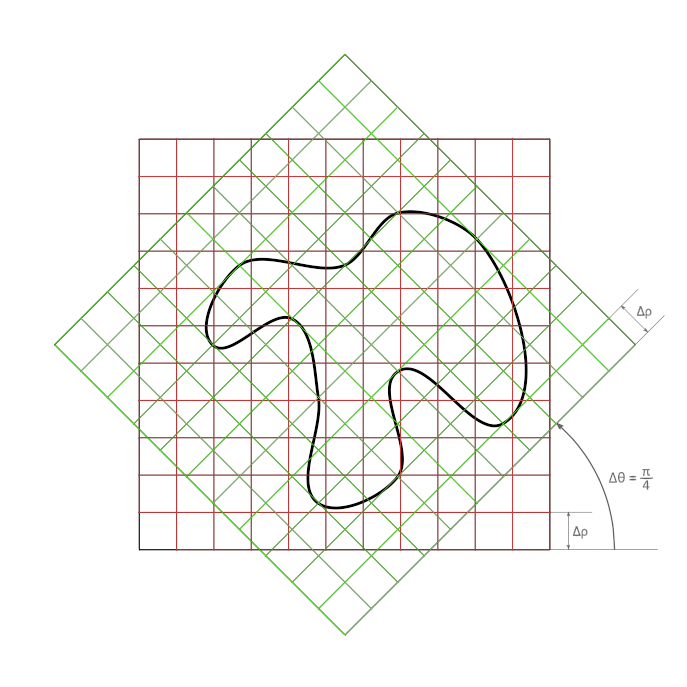
\includegraphics[width=0.45\columnwidth]{chan_vese_length.png}
		\label{fig:chanveselength}
	}
	\subfigure[]
	{
		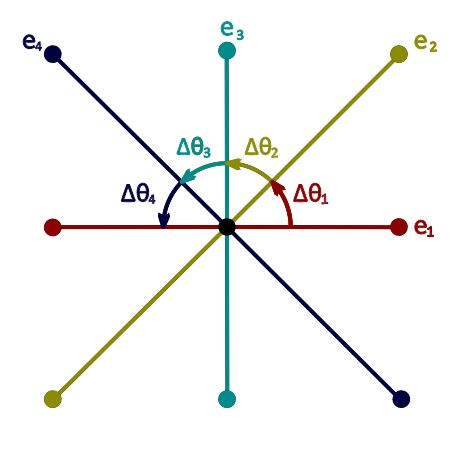
\includegraphics[width=0.45\columnwidth]{chan_vese_cauchycrofton.png}
		\label{fig:chanvesediscretelength}
	}
	\caption{\textbf{(a)} Cauchy-Crofton length approximation. \textbf{(b)} 8-connected neighbourhood system.}
	\label{fig:chanveseN8}
\end{figure}

\begin{definition}[Discrete Representation of Mumford-Shah Function]
	With the exception of the second term in \Cref{eq:mumfordshahfunction}, the remaining terms are represented easily discretely. For each pixel $p \in \Omega$, let $x_p$ be a binary variable such that
	\begin{equation}
		x_p = 
		\begin{cases} 
			0 & \phi(p)\leq 0 \\
			1 & \phi(p)> 0
		\end{cases}
	\end{equation}
	The means can now be calculated using 
	\begin{equation}
		c_1 = \frac{\sum_p u(x,y)x_p}{\sum_p x_p},
	\end{equation}
	\begin{equation}
		c_2 = \frac{\sum_p u(x,y)(1-x_p)}{\sum_p (1-x_p)}.
	\end{equation}
	For simplification, $\nu=0$. To determine contour length using an 8-neighbourhood system, as illustrated in \Cref{fig:chanvesediscretelength}, we set $\Delta\rho=1$. The weight $w_k$ is assigned to it's corresponding edge $e_k$. The Euclidean length of the  edges is $|e_1|=|e_3| = 1$ and $|e_2|=|e_4|=\sqrt{2}$, therefore the corresponding weights, which are determined using \Cref{eq:discretelength}, is $w_1 = w_3 = \frac{\pi}{8}$ and $w_2 = w_4 = \frac{\pi}{8\sqrt{2}}$. To calculate $n_k$ we need to count the intersections between the lines and the contour. An intersection between two pixels $p$ and $q$ exists \textit{if and only if} $x_p$ and $x_q$ have different labels.
	\begin{equation}
		n_{k} = x_p(1-x_q) + x_q(1-x_p) \text{; } \, k={(pq) \in \mathcal{N}_p}. 
	\end{equation}
	The contour length can now fully be expressed discretely as 
	\begin{equation}
		\lVert C \rVert_E = \sum_{p,q \in e_k} w_k( x_p(1-x_q) + x_q(1-x_p)).
	\end{equation}
	
	The discrete representation of \Cref{eq:mumfordshahfunction} is
	\begin{equation}
		\begin{split}
			F(x_1, \ldots, x_n) & = \mu \sum_{p,q \in e_k} w_k( x_p(1-x_q) + x_q(1-x_p)) \\
			& + \lambda_1 \sum_p |u(x,y)-c_1|^2x_p \\
			& + \lambda_2 \sum_p |u(x,y)-c_2|^2(1-x_p)
		\end{split}
		\label{eq:discretemumfordshah}
	\end{equation}
\end{definition}

\begin{definition}[Graph Representation] The discrete energy function \Cref{eq:discretemumfordshah} has been shown that it obey the submodularity constraint for graph representability. Therefore the data energy and regularistion energy is
	\begin{equation}
		E^p(x_p) = \lambda_1 |u(x,y)-c_1|^2 x_p + \lambda_2 |u(x,y)-c_2|^2 (1-x_p)
	\end{equation}
	\begin{equation}
	E^{pq}(x_p,x_q) = (x_p + x_q - 2x_px_q)w_{pq}
	\end{equation}
\end{definition}
The graph for the energy function is constructed as in \citep{Kolmogorov2004}.

\section{Modified Weighting and Parameter Estimation}
\label{sec:cvgc_weightingandparameterestimation}

\textcolor{red}{What is wrong with the previously described graph weighting. What would we expect from a better weighting system. Problem images are multi-modal and extremely low contrast.}
In this section we introduce a novel idea to weighting  a graph for image segmentation based on the Chan-Vese formulation of the Mumford-Shah evolution function. Previous parameter estimation schemes focused very specifically on a certain image and this resutled in hard-coded. In \citep{ElZehiry2007}, were this method was first devised, they used the parameter settings $\mu = 0.1 \times 255^2$, $\lambda_1 = \lambda_2 = 1$. This worked very well on their synthetic images proving a strong resilience to noise and initial conditions. However, for fluorescence microscopy images, the results to be a bit too over-segemented for practical use. These parameters were used to segment the images in the sample set, \Cref{fig:sampleset}, the segmentation result is shown in \Cref{fig:samplesetdefaultcv}.

\begin{figure}[!h]
	\centering
	\subfigure[]
	{
		\includegraphics[width=0.3\columnwidth]{default_cv/1gray.jpg}
		\label{fig:1graydefaultcv}
	}
	\subfigure[]
	{
		\includegraphics[width=0.3\columnwidth]{default_cv/2gray.jpg}
		\label{fig:2graydefaultcv}
	}
	\subfigure[]
	{
		\includegraphics[width=0.3\columnwidth]{default_cv/3gray.jpg}
		\label{fig:3graydefaultcv}
	}
	\subfigure[]
	{
		\includegraphics[width=0.3\columnwidth]{default_cv/4gray.jpg}
		\label{fig:4graydefaultcv}
	}
	\subfigure[]
	{
		\includegraphics[width=0.3\columnwidth]{default_cv/5gray.jpg}
		\label{fig:5graydefaultcv}
	}
	\subfigure[]
	{
		\includegraphics[width=0.3\columnwidth]{default_cv/6gray.jpg}
		\label{fig:6graydefaultcv}
	}
	\caption{CAPTION MISSING HERE.}
	\label{fig:samplesetdefaultcv}
\end{figure}

In \citep{Maska2013}, the authors propsed a segmentation and tracking scheme for whole fluorescent cells in a timelapse series. The result was another set of hard-coded parameters which were based on maximising the Jacard coefficient of the automatically segmented cells in each frame of the timelapse series which was also manually segmented. The optimal parameter settings were $\mu=0.01$, $\lambda_1=1$ and $\lambda_2 = 85$. These parameters were used on the sample set in \Cref{fig:sampleset} and the results proved to be less useful as shown in \Cref{fig:samplesetcelltrack}. It can be deduced that the parameters were specifically tuned to the image type that was studied.

\begin{figure}[!t]
	\centering
	\subfigure[]
	{
		\includegraphics[width=0.3\columnwidth]{cell_tracking/1gray.jpg}
		\label{fig:1graycelltrack}
	}
	\subfigure[]
	{
		\includegraphics[width=0.3\columnwidth]{cell_tracking/2gray.jpg}
		\label{fig:2graycelltrack}
	}
	\subfigure[]
	{
		\includegraphics[width=0.3\columnwidth]{cell_tracking/3gray.jpg}
		\label{fig:3graycelltrack}
	}
	\subfigure[]
	{
		\includegraphics[width=0.3\columnwidth]{cell_tracking/4gray.jpg}
		\label{fig:4graycelltrack}
	}
	\subfigure[]
	{
		\includegraphics[width=0.3\columnwidth]{cell_tracking/5gray.jpg}
		\label{fig:5graycelltrack}
	}
	\subfigure[]
	{
		\includegraphics[width=0.3\columnwidth]{cell_tracking/6gray.jpg}
		\label{fig:6graycelltrack}
	}
	\caption{CAPTION MISSING HERE.}
	\label{fig:samplesetcelltrack}
\end{figure}

It can be seen that hard-coded parameter values do not produce very consistent results over a large range of image types as that found in fluorescence microscopy imaging. In the next section, \Cref{sec:cvgc_weighting} we devise a novel weighting scheme, parameter estimation as well as a new way to think of the parameters involved, in terms of \textit{proxy parameters}. We then specifically focus on tuning these parameter for fluorescence images in \Cref{sec:cvgc_parameterestimation}.

\subsection{Graph Weighting}
\label{sec:cvgc_weighting}

The first thing we do is normalise the weighting for both the data and smoothing connections. For the weighting of the neighbourhood connections we use the Euclidean distance between adjacent nodes. This results in neigbourhood connections as illustrated in \Cref{fig:singlenodeconstruction}. The range of pixel intensities is also normlised i.e. $p \in [0,1]$. The weight of the connection from the source to the node $p$ is given by $E^i(0)|_{i=p} = \lambda_0|p-c_0|^2$. This is seen as how far away the pixel is from $c_0$. Similarly, the weight of the connection from the node to the sink is given by $E^i(1)|_{i=p}=\lambda_1|p-c_1|^2$, i.e. how far way the pixel is from $c_1$. The fully connected graph for a single node in te 8-connected neighbourhood system is illustrated in \Cref{fig:singlenodeconstruction}.

\tikzstyle{vertex}=[circle,thick,draw]
\begin{figure}[!h]
	\centering
	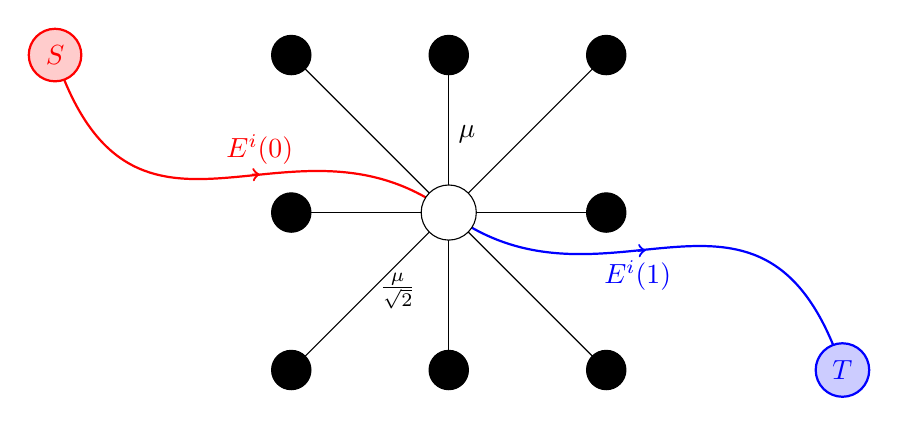
\begin{tikzpicture}[scale=1.0]
	\draw (0,0) -- (2,0);
	\draw (0,0) -- (-2,0);
	\draw (0,0) -- (0,1) node[right] {$\mu$} -- (0,2);
	\draw (0,0) -- (0,-2);
	
	\draw (0,0) -- (-2,2);
	\draw (0,0) -- (2,2);
	\draw (0,0) -- (-1,-1) node[right] {$\frac{\mu}{\sqrt{2}}$} -- (-2,-2);
	\draw (0,0) -- (2,-2);
	
	\draw[red,thick] (-5,2) .. controls(-4,-1) and (-2,1.5) .. (0,0);
	\draw[red,->,thick] (-2.5,0.48) -- (-2.4,0.485) node[above] {$E^i(0)$};
	\node[vertex,red,fill=red!20] at (-5,2) {$S$};
	\draw[blue,thick] (5,-2) .. controls(4,1) and (2,-1.5) .. (0,0);
	\draw[blue,<-,thick] (2.5,-0.48) -- (2.4,-0.485) node[below] {$E^i(1)$};
	\node[vertex,blue,fill=blue!20] at (5,-2) {$T$};
	
	\draw[fill=white] (0,0) circle (0.35);
	\draw[fill=black] (-2,0) circle (0.25);
	\draw[fill=black] (2,0) circle (0.25);
	
	\draw[fill=black] (0,2) circle (0.25);
	\draw[fill=black] (-2,2) circle (0.25);
	\draw[fill=black] (2,2) circle (0.25);
	
	\draw[fill=black] (0,-2) circle (0.25);
	\draw[fill=black] (-2,-2) circle (0.25);
	\draw[fill=black] (2,-2) circle (0.25);
	\end{tikzpicture}
	\caption{Fully connected single node.}
	\label{fig:singlenodeconstruction}
\end{figure}

\textcolor{red}{Describe the modified weighting and parameter relations.}

\subsection{Analysis of Weighting System and Parameter Relationships}
\label{sec:cvgc_analysis}

\textcolor{red}{Describe the relationship between various parameters including their limits and ranges.}

To better understand the relationship between $\lambda_0$ and $\lambda_1$ and its impact on the final solution we explicitely formalise the dependancy and set
\begin{equation}
	\lambda_0 = \alpha\lambda_1.
	\label{eq:l0l1dependancy}
\end{equation}
Forcing this relation between $\lambda_0$ and $\lambda_1$ makes further analysis simpler and more intuitive. We can immediately see a constraint on $\alpha$. Since, we require data connections to be positive, i.e. $E^i(0), E^i(1) \geq 0$ (SEE SECTION??), this gives us a lowerbound on $\alpha$ for positive concavity of the energy functions
\begin{equation}
	\alpha > 0 \,\text{ lowerbound on } \alpha
\end{equation}

We will now analyse the flow through a single node. We use  \Cref{fig:singlenodeconstruction} to facilitate our explanation. From the neighbourhood connections, in an 8-connected neihgbourhood construction, the maximum flow into or out of a node to its neighbours is 
\begin{equation}
	f_{max} = 4\mu + 4\frac{\mu}{\sqrt{2}} = \mu \left( 2\sqrt{2} + 4\right).
	\label{eq:neighbourhoodsaturation}
\end{equation}
To guarantee that a node $p$ will be place in the source set, $p \in S$, we know that the incoming flow from the source must completely saturate all flow outlets, this can be expressed as
\begin{equation}
	E^i(0) > E^i(1) + \mu \left( 2\sqrt{2} + 4\right).
	\label{eq:sourcesaturation}
\end{equation}
This can be read as \textit{"The source saturates the sink and all neighbourhood connections"}.
Similarly to guarantee the node will be in the sink set, $p \in T$
\begin{equation}
E^i(1) > E^i(0) + \mu \left( 2\sqrt{2} + 4\right).
\end{equation}
This can be read as \textit{"The sink is larger than the source and all neighbourhood connections"}. To aid in understanding the energies we use \Cref{fig:dataenergyplot}.

For quadratic energies with $0 < c_0 < c_1 < 1$, there is a point, between $c_0$ and $c_1$, where the incoming flow from the source is completely saturates the sink with no excess remaining. This point, where the energies are equal, we call $p_e$, i.e. $E_0(p_e) = E_1(p_e)$. This point of zero net flow can be found as follows
\begin{equation*}\begin{split}
	E^{i=p_e}(1) & = E^{i=p_e}(0) \\
	\lambda_1(p_e - c_1)^2 & = \lambda_0(p_e - c_0)^2 \\
	\frac{(p_e - c_0)^2}{(p_e - c_1)^2} & = \frac{\lambda_1}{\lambda_0}\\
	\frac{p_e - c_0}{p_e - c_1}  = \sqrt{\frac{\lambda_1}{\lambda_0}} \hspace{20pt}&\text{or}\hspace{20pt}\frac{p_e - c_0}{p_e - c_1}  = -\sqrt{\frac{\lambda_1}{\lambda_0}}
\end{split}\end{equation*}
We know that 
\begin{equation*}\begin{split}
	c_0 < &\,\, p_e < c_1 \\
	\therefore p_e-c_0 >0 \hspace{20pt}&\text{and}\hspace{20pt} p_e-c_1 < 0 
\end{split}\end{equation*}
It follows directly that
\begin{equation*}\begin{split}
	\frac{p_e-c_1}{p_e-c_0} &= -\sqrt{\frac{\lambda_1}{\lambda_0}} \\
	\frac{(p_e-c_0)+(c_0-c_1)}{p_e-c_0} &= -\sqrt{\frac{\lambda_1}{\lambda_0}}\\
	\frac{c_0-c_1}{p_e-c_0} &= -\left( \sqrt{\frac{\lambda_1}{\lambda_0}} + 1\right)\\
	p_e = c_0 + \frac{c_1-c_0}{\sqrt{\frac{\lambda_1}{\lambda_0}} + 1}
\end{split}\end{equation*}
After substituting the relation in \Cref{eq:l0l1dependancy} we get
\begin{equation}
	p_e = c_0 + \frac{c_1-c_0}{\sqrt{\alpha} + 1}
	\label{eq:pe}
\end{equation}
The point where the energies are equal, $p_e$, is shown in \Cref{fig:dataenergyplot}.

\begin{figure}[!t]
	\centering
	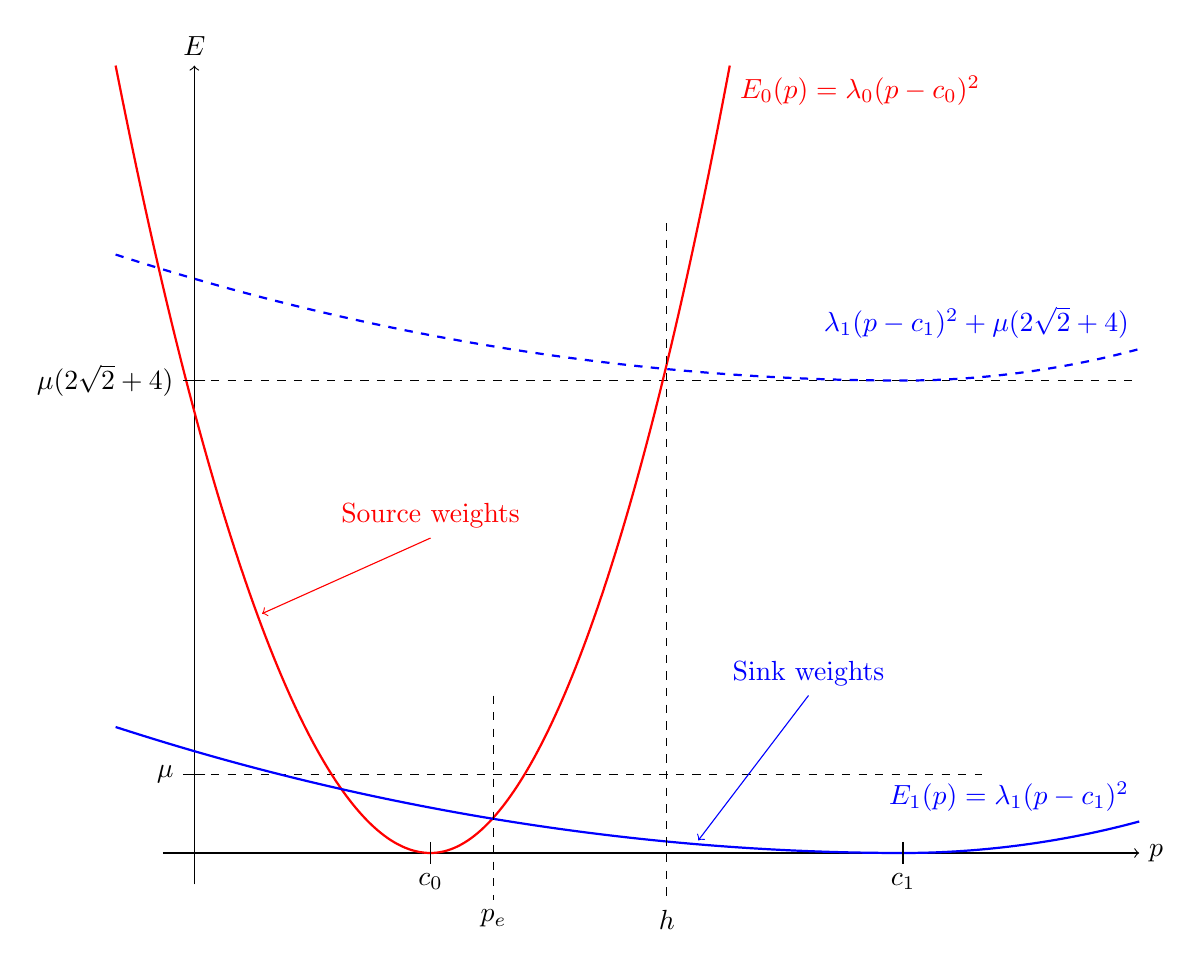
\begin{tikzpicture}[scale=2]
	\draw[->] (-0.2,0) -- (6,0) node[right] {$p$};
	\draw[->] (0,-0.2) -- (0,5) node[above] {$E$};
	
	\draw[dashed] (0,0.5) -- (5,0.5);
	\draw[dashed] (0,3) -- (6,3);
	\draw[red,thick] (-0.5,5) parabola bend (1.5,0) (3.4,5) node[below right] {$E_0(p) = \lambda_0 (p-c_0)^2$};
	\draw[blue,thick] (-0.5,0.8) parabola bend (4.5,0) (6,0.2) node[above left] {$E_1(p) = \lambda_1 (p-c_1)^2$};
	\draw[dashed,blue,thick] (-0.5,3.8) parabola bend (4.5,3) (6,3.2) node[above left] {$\lambda_1 (p-c_1)^2 + \mu(2\sqrt{2}+4)$};
	\draw[shift={(1.5,0)}] (0pt,2pt) -- (0pt,-2pt) node[below] {$c_0$};
	\draw[shift={(4.5,0)}] (0pt,2pt) -- (0pt,-2pt) node[below] {$c_1$};
	\draw[shift={(0,0.5)}] (2pt,0pt) -- (-2pt,0pt) node[left] {$\mu$};
	\draw[shift={(0,3)}] (2pt,0pt) -- (-2pt,0pt) node[left] {$\mu(2\sqrt{2}+4)$};
	
	\draw[dashed,black] (3.0,4) -- (3.0,-0.3) node[below] {$h$};
	\draw[dashed,black] (1.9,1) -- (1.9,-0.3) node[below] {$p_e$};
	%\draw[dashed,black] (0.94,1) -- (0.94,-0.3) node[below] {$p_e$};
	
	\draw[red,<-] (0.43,1.52) -- (1.5,2) node[above] {Source weights};
	\draw[blue,<-] (3.2,0.08) -- (3.9,1) node[above] {Sink weights};
	\end{tikzpicture}
	\caption{Data energy functions plot.}
	\label{fig:dataenergyplot}
\end{figure}

\begin{definition}[Analysis of the relationship between $p_e$ and $\alpha$]
	From \Cref{eq:pe} we note that there is one tunable parameter, i.e. $\alpha$. We can see that $p_e$ and $\alpha$ are inversely related. This is expressed mathematically as
\begin{equation*}\begin{split}
		\text{if } \alpha=1, p_e=c_0+\frac{c_1-c_0}{1+\sqrt{1}} = \frac{c_0+c_1}{2} \hspace{30pt}&\text{(midpoint between $c_0$ and $c_1$)}\\
		\lim_{\alpha\to\infty}p_e = \lim_{\alpha\to\infty}c_0+\frac{c_1-c_0}{1+\sqrt{\infty}} = c_0\hspace{30pt} &\text{(maximum $\alpha$ yields lowerbound on $p_e$)}\\
		\lim_{\alpha\to0}p_e = \lim_{\alpha\to0}c_0+\frac{c_1-c_0}{1+\sqrt{0}} = c_1\hspace{30pt} &\text{(minimum $\alpha$ yields upperbound on $p_e$)}
	\end{split}\end{equation*}
\end{definition}
The relationship between $p_e$ and $\alpha$ is illustrated in \Cref{fig:alphaperelationship}.
\begin{figure}[!h]
	\centering
	\begin{tikzpicture}[scale=1]
	\draw[->] (0,0) -- (15,0) node[right] {$p$};
	\draw[shift={(3,0)}] (0pt,4pt) -- (0pt,-4pt) node[below] {$c_0$};
	\draw[shift={(12,0)}] (0pt,4pt) -- (0pt,-4pt) node[below] {$c_1$};
	\draw[dashed,black] (7.5,1.5) node[above] {$p_e = \frac{c_0+c_1}{2}$} -- (7.5,-0.3) node[below] {$\alpha=1$};
	\draw[black,->,thick] (7.5,0.5) -- (5.5,0.5) node[above] {increasing $\alpha$} -- (4.5,0.5);
	\draw[black,->,thick] (7.5,0.5) -- (9.5,0.5) node[above] {decreasing $\alpha$} -- (10.5,0.5);
	\end{tikzpicture}
	\caption{Relationship between $\alpha$ and $p_e$.}
	\label{fig:alphaperelationship}
\end{figure}

\begin{definition}[Figuring $\alpha$]
	If we are able to make good estimates on $p_e$, $c_0$ and $c_1$ for the final segmented image, then it is possible to calculate $\alpha$ as follows:
	\begin{equation*}\begin{split}
		p_e &= c_0 + \frac{c_1-c_0}{\sqrt{\alpha} + 1} \\
		1+\sqrt{\alpha} &= \frac{c_1-c_0}{p_e-c_0}
		%\alpha &= \left( \frac{c_1-c_0}{p_e-c_0}-1 \right)^2
	\end{split}\end{equation*}
	\begin{equation}
		\alpha = \left( \frac{c_1-c_0}{p_e-c_0}-1 \right)^2
		\label{eq:alphaapproximation}
	\end{equation}
\end{definition}

\begin{definition}[Lowerbound on $\mu$]
	When we found the point, $p_e$, where the energies are equal in \Cref{eq:pe}, we ignored the other solution as it was not within the range from $c_0$ to $c_1$. Let this point be $p_{e^*}$. If this point is positive and $0<p_{e^*}<c_0$ then we must ensure that at no point within this range that the source flow saturates all the outgoing edges. This force a limit on how low $\mu$ can be. This is only of significant concern when $\alpha>1$. We only need to concern ourselve with the point $p=0$ as this is the point where the difference $E^i(0)-E^i(1)$ is the largest. The lowerbound on $\mu$ can be obtained as follows
	\begin{equation*}\begin{split}
		E^i(0)|_{p_i=0} &< E^i(1)|_{p_i=0} + \mu \left( 2\sqrt{2} + 4\right) \\
		\lambda_0c_0^2 &< \lambda_1c_1^2 + \mu \left( 2\sqrt{2} + 4\right) \\
		\therefore \mu \left( 2\sqrt{2} + 4\right) &> \lambda_0c_0^2 - \lambda_1c_1^2\\
		\mu &> \frac{\lambda_0c_0^2 - \lambda_1c_1^2}{\left( 2\sqrt{2} + 4\right)}
	\end{split}\end{equation*} 
\end{definition}
Taking into account the relation in \Cref{eq:l0l1dependancy} this becomes
\begin{equation}
	\mu > \frac{\lambda_1(\alpha c_0^2-c_1^2)}{\left( 2\sqrt{2} + 4\right)}
	\label{eq:mulowerbound}
\end{equation}

\begin{definition}[Absolutely in the source set] From \Cref{eq:sourcesaturation} we can see that there is a point beyond which all nodes which correspond to pixel value higher than that point will be saturated and have excess flow which means that they will be in the source set. We will call this point the \textit{saturation point} and denote it by $h$. This is shown in \Cref{fig:dataenergyplot}. This point can be determined as follows:
\begin{equation*}\begin{split}
	\lambda_0(h-c_0)^2 &> \lambda_1(h-c_1)^2 + f_{max} \\
	\lambda_0(h-c_0)^2 - \lambda_1(h-c_1)^2 &> f_{max} \\
	(\lambda_0-\lambda_1)h^2 + (-2\lambda_0 c_0 + 2\lambda_1 c_1)h + (\lambda_0 c_0^2 - \lambda_1 c_1^2-f_{max}) &> 0
\end{split}\end{equation*}
The solutions to $h$ are
\begin{equation*}\begin{split}
	h = \frac{ (2\lambda_0 c_0 - 2\lambda_1 c_1) \pm \sqrt{(-2\lambda_0 c_0 + 2\lambda_1 c_1)^2-4(\lambda_0-\lambda_1)(\lambda_0 c_0^2 - \lambda_1 c_1^2-f_{max})}}{2(\lambda_0-\lambda_1)}
\end{split}\end{equation*}
Substituting the relation in \Cref{eq:l0l1dependancy}
\begin{equation*}\begin{split}
	h &= \frac{(\alpha c_0-c_1)\pm\sqrt{(c_1-\alpha c_0)^2-(\alpha-1)(\alpha c_0^2-c_1^2-\frac{f_{max}}{\lambda_1})}}{\alpha-1}\\
	&= \frac{(\alpha c_0-c_1)\pm\sqrt{\alpha(c_0-c_1)^2+\frac{f_{max}}{\lambda_1}(\alpha-1)}}{\alpha-1}
\end{split}\end{equation*}
If the $\mu$ is greater than the lowerbound in \Cref{eq:mulowerbound} then there is only one solution to $h$ which is of importance. This is the positive solution for $h$ which is
\begin{equation}
	h = \frac{(\alpha c_0-c_1)+\sqrt{\alpha(c_0-c_1)^2+\frac{\mu(2\sqrt{2}+4)}{\lambda_1}(\alpha-1)}}{\alpha-1}
	\label{eq:h}
\end{equation}
This point is marked off in \Cref{fig:dataenergyplot}.
\end{definition}

\begin{definition}[Determining $\lambda_1$] Given good approximations for $c_0$, $c_1$, $\alpha$, $h$ and $\mu$, we can calculate the appropriate value for $\lambda_1$. We proceed from \Cref{eq:sourcesaturation} as follows
\begin{equation*}\begin{split}
	\lambda_0(h-c_0)^2 &= \lambda_1(h-c_1)^2 + \mu(2\sqrt{2}+4)\\
	\lambda_1 \left( \alpha(h-c_0)^2-(h-c_1)^2 \right) &= \mu(2\sqrt{2}+4)
\end{split}\end{equation*}
\begin{equation}
	\lambda_1 = \frac{\mu(2\sqrt{2}+4)}{\alpha(h-c_0)^2-(h-c_1)^2}
	\label{eq:lambda1approximation}
\end{equation}
\end{definition}

\begin{definition}[Parameter estimation process]
	The parameter estimation is based on the assumption that sufficiently good approximations for $c_0$, $c_1$, $p_e$ and $h$ can be obtained. By sufficiently good we are referring to the closeness to the values these parameters would take for an ideal segmetation. From these approximations, we calculate the approximation for $\alpha$ using \Cref{eq:alphaapproximation}. The parameters $\mu$ and $\lambda_1$ are related and aren't seperable, therefore we set choose to set $\mu$. We can then calculate $\lambda_1$ using \Cref{eq:lambda1approximation}. For the chosen $\mu$ we can calculate the upperbound on $\lambda_1$ to ensure that the constraint \Cref{eq:mulowerbound} is met. The constraint on $\lambda_1$ is calculated as follows
\begin{equation*}
\mu\left( 2\sqrt{2} + 4 \right) > \lambda_1(\alpha c_0^2 - c_1^2)
\end{equation*}
\begin{equation}
	\lambda_1 < \frac{\mu\left( 2\sqrt{2} + 4 \right)}{\alpha c_0^2 - c_1^2}
\end{equation}
Finally $\lambda_0$ can be calculated using \Cref{eq:l0l1dependancy}.
\end{definition}

\subsection{Tuning Parameters for Fluorescence Microscopy}
\label{sec:cvgc_parameterestimation}

\textcolor{red}{What sort of image properties are we tuning for? E.g. dark bg, low contrast, etc. Parameters limits and ranges.} The properties of the images obtained in fluorescence microscopy imaging can be used to guide the parameter estimation process. We focus, specifically, on black background images. Due to the fact that the predominant form of noise in the imaging system in Poisson distributed, we can further assume that the darker the background, the less noise that is present therein. The Poisson process also tells us that brighter regions exhibit a greater intensity variation due to the sampling process. Therefore, the curve for $E^i(1)$ is less convex than $E^i(0)$ as in \Cref{fig:dataenergyplot} and, resultantly, the value for $p_e$, in \Cref{fig:alphaperelationship}, is shifted to the left. This places a new lowerbound on $\alpha$ for fluorescence images
\begin{equation}
	\alpha \geq 1.
	\label{eq:alphalowerboundFM}
\end{equation}

\begin{definition}[Manual Tuning] Before moving further into analysis of the relationships between the parameters, we first peform a manual tuning of parameters and observing the effect on the segmented results. This allows us to understand how strongly correlated the parameter is to the final result. We note that the curves, $E^i(0)$ and $E^i(1)$, can be tuned relative to a fixed value for $\mu$ and this wouldn't impact significantly on the range of possible solution sets. Therefore, we set $\mu=1$ in all our manual parameter tuning. We use a stopping criterion of $\epsilon=1\times10^{-3}$.
	
We cover a relatively wide range of parameter settings and note the output, i.e. over-segmented, under-segmented, almost ideal, etc. At this point, catergorising the segemented output is largely subjective. We also use various initial conditions. Specifically, we use the segmented output from Otsu binarization, K-means ($k=2$) and Expectation-Maximisation for Gaussian Mixture Modelling (EMGMM) with ($k=2$). The initial and final means are of significant important in this study.

For \Cref{fig:1gray}, we used show the output for the following combinations of $\alpha$ and $\lambda_1$. $(\alpha,\lambda_1) = \{(30,150), (40,50), (40,100), (40,150), (40,200), (45,150), (50,150)\}$. The initial segmentation masks are shown in \Cref{fig:image1init}. The segmented output for the combinations are shown in \Cref{fig:image1mytune}.

For \Cref{fig:2gray}, we used show the output for the following combinations of $\alpha$ and $\lambda_1$. $(\alpha,\lambda_1) = \{(30,150), (40,50), (40,100), (40,150), (40,200), (45,150), (50,150)\}$. The initial segmentation masks are shown in \Cref{fig:image2init}. The segmented output for the combinations are shown in \Cref{fig:image2mytune}.

For \Cref{fig:3gray}, we used show the output for the following combinations of $\alpha$ and $\lambda_1$. $(\alpha,\lambda_1) = \{(1,150), (10,150), (10,200), (10,400), (10,800), (20,150), (30,150), (40,150), (50,150)\}$. The initial segmentation masks are shown in \Cref{fig:image3init}. The segmented output for the combinations are shown in \Cref{fig:image3mytune}.

For \Cref{fig:4gray}, we used show the output for the following combinations of $\alpha$ and $\lambda_1$. $(\alpha,\lambda_1) = \{(30,50), (30,100), (30,150), (40,100), (40,150), (50,150)\}$. The initial segmentation masks are shown in \Cref{fig:image4init}. The segmented output for the combinations are shown in \Cref{fig:image4mytune}.

For \Cref{fig:5gray}, we used show the output for the following combinations of $\alpha$ and $\lambda_1$. $(\alpha,\lambda_1) = \{(30,50), (30,100), (30,150), (40,100), (40,150), (50,150)\}$. The initial segmentation masks are shown in \Cref{fig:image5init}. The segmented output for the combinations are shown in \Cref{fig:image5mytune}.

For \Cref{fig:6gray}, we used show the output for the following combinations of $\alpha$ and $\lambda_1$. $(\alpha,\lambda_1) = \{(20,20), (20,150), (30,150), (40,50), (40,150), (50,150)\}$. The initial segmentation masks are shown in \Cref{fig:image6init}. The segmented output for the combinations are shown in \Cref{fig:image6mytune}.

The means and standard deviations for the initial masks obtained are shown in \Cref{tab:initmaskvalues}.

\clearpage

\begin{figure}[!t]
	\centering
	\subfigure[Otsu]
	{
		\includegraphics[width=0.3\columnwidth]{mymanualtuning/image1/otsu_init.jpg}
		\label{fig:1grayotsu}
	}
	\subfigure[K-Means ($k=2$)]
	{
		\includegraphics[width=0.3\columnwidth]{mymanualtuning/image1/kmeans_init.jpg}
		\label{fig:1graykmeans}
	}
	\subfigure[EMGMM ($k=2$)]
	{
		\includegraphics[width=0.3\columnwidth]{mymanualtuning/image1/emgmm_init.jpg}
		\label{fig:1grayemgmm}
	}
	\caption{Image 1 from sample set \Cref{fig:sampleset} initial masks.}
	\label{fig:image1init}
\end{figure}

\begin{figure}[!t]
	\centering
	\subfigure[$\mu=1$, $\alpha=30$, $\lambda_1=150$]
	{
		\includegraphics[width=0.3\columnwidth]{mymanualtuning/image1/1_30_150.jpg}
		\label{fig:1graymytune1}
	}
	\subfigure[$\mu=1$, $\alpha=40$, $\lambda_1=50$]
	{
		\includegraphics[width=0.3\columnwidth]{mymanualtuning/image1/1_40_50.jpg}
		\label{fig:1graymytune2}
	}
	\subfigure[$\mu=1$, $\alpha=40$, $\lambda_1=100$]
	{
		\includegraphics[width=0.3\columnwidth]{mymanualtuning/image1/1_40_100.jpg}
		\label{fig:1graymytune3}
	}
	\subfigure[$\mu=1$, $\alpha=40$, $\lambda_1=150$]
	{
		\includegraphics[width=0.3\columnwidth]{mymanualtuning/image1/1_40_150.jpg}
		\label{fig:1graymytune4}
	}
	\subfigure[$\mu=1$, $\alpha=40$, $\lambda_1=200$]
	{
		\includegraphics[width=0.3\columnwidth]{mymanualtuning/image1/1_40_200.jpg}
		\label{fig:1graymytune5}
	}
%	\subfigure[$\mu=1$, $\alpha=45$, $\lambda_1=150$]
%	{
%		\includegraphics[width=0.3\columnwidth]{mymanualtuning/image1/1_45_150.jpg}
%		\label{fig:1graymytune6}
%	}
	\subfigure[$\mu=1$, $\alpha=50$, $\lambda_1=150$]
	{
		\includegraphics[width=0.3\columnwidth]{mymanualtuning/image1/1_50_150.jpg}
		\label{fig:1graymytune7}
	}
	\caption{Segmented output for various combination of $\alpha$ and $\lambda_1$ for Image 1 in the sample set.}
	\label{fig:image1mytune}
\end{figure}

\begin{figure}[!t]
	\centering
	\subfigure[Otsu]
	{
		\includegraphics[width=0.3\columnwidth]{mymanualtuning/image2/otsu_init.jpg}
		\label{fig:2grayotsu}
	}
	\subfigure[K-Means ($k=2$)]
	{
		\includegraphics[width=0.3\columnwidth]{mymanualtuning/image2/kmeans_init.jpg}
		\label{fig:2graykmeans}
	}
	\subfigure[EMGMM ($k=2$)]
	{
		\includegraphics[width=0.3\columnwidth]{mymanualtuning/image2/emgmm_init.jpg}
		\label{fig:2grayemgmm}
	}
	\caption{Image 2 from sample set \Cref{fig:sampleset} initial masks.}
	\label{fig:image2init}
\end{figure}

\begin{figure}[!t]
	\centering
	\subfigure[$\mu=1$, $\alpha=30$, $\lambda_1=150$]
	{
		\includegraphics[width=0.3\columnwidth]{mymanualtuning/image2/1_30_150.jpg}
		\label{fig:2graymytune1}
	}
	\subfigure[$\mu=1$, $\alpha=40$, $\lambda_1=50$]
	{
		\includegraphics[width=0.3\columnwidth]{mymanualtuning/image2/1_40_50.jpg}
		\label{fig:2graymytune2}
	}
%	\subfigure[$\mu=1$, $\alpha=40$, $\lambda_1=100$]
%	{
%		\includegraphics[width=0.3\columnwidth]{mymanualtuning/image2/1_40_100.jpg}
%		\label{fig:2graymytune3}
%	}
	\subfigure[$\mu=1$, $\alpha=40$, $\lambda_1=150$]
	{
		\includegraphics[width=0.3\columnwidth]{mymanualtuning/image2/1_40_150.jpg}
		\label{fig:2graymytune4}
	}
	\subfigure[$\mu=1$, $\alpha=40$, $\lambda_1=200$]
	{
		\includegraphics[width=0.3\columnwidth]{mymanualtuning/image2/1_40_200.jpg}
		\label{fig:2graymytune5}
	}
	\subfigure[$\mu=1$, $\alpha=45$, $\lambda_1=150$]
	{
		\includegraphics[width=0.3\columnwidth]{mymanualtuning/image2/1_45_150.jpg}
		\label{fig:2graymytune6}
	}
	\subfigure[$\mu=1$, $\alpha=50$, $\lambda_1=150$]
	{
		\includegraphics[width=0.3\columnwidth]{mymanualtuning/image2/1_50_150.jpg}
		\label{fig:2graymytune7}
	}
	\caption{Segmented output for various combination of $\alpha$ and $\lambda_1$ for Image 2 in the sample set.}
	\label{fig:image2mytune}
\end{figure}

\begin{figure}[!t]
	\centering
	\subfigure[Otsu]
	{
		\includegraphics[width=0.3\columnwidth]{mymanualtuning/image3/otsu_init.jpg}
		\label{fig:3grayotsu}
	}
	\subfigure[K-means ($k=2$)]
	{
		\includegraphics[width=0.3\columnwidth]{mymanualtuning/image3/kmeans_init.jpg}
		\label{fig:3graykmeans}
	}
	\subfigure[EMGMM ($k=2$)]
	{
		\includegraphics[width=0.3\columnwidth]{mymanualtuning/image3/emgmm_init.jpg}
		\label{fig:3grayemgmm}
	}
	\caption{Image 3 from sample set \Cref{fig:sampleset} initial masks.}
	\label{fig:image3init}
\end{figure}

\begin{figure}[!t]
	\centering
	\subfigure[$\mu=1$, $\alpha=1$, $\lambda_1=150$]
	{
		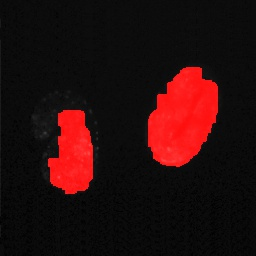
\includegraphics[width=0.3\columnwidth]{mymanualtuning/image3/1_1_150.jpg}
		\label{fig:3graymytune1}
	}
%	\subfigure[$\mu=1$, $\alpha=10$, $\lambda_1=150$]
%	{
%		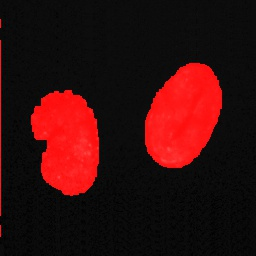
\includegraphics[width=0.3\columnwidth]{mymanualtuning/image3/1_10_150.jpg}
%		\label{fig:3graymytune2}
%	}
%	\subfigure[$\mu=1$, $\alpha=10$, $\lambda_1=200$]
%	{
%		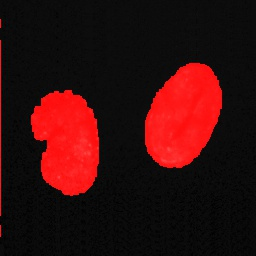
\includegraphics[width=0.3\columnwidth]{mymanualtuning/image3/1_10_200.jpg}
%		\label{fig:3graymytune3}
%	}
	\subfigure[$\mu=1$, $\alpha=10$, $\lambda_1=400$]
	{
		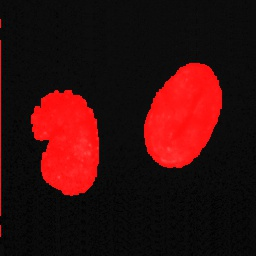
\includegraphics[width=0.3\columnwidth]{mymanualtuning/image3/1_10_400.jpg}
		\label{fig:3graymytune4}
	}
	\subfigure[$\mu=1$, $\alpha=10$, $\lambda_1=800$]
	{
		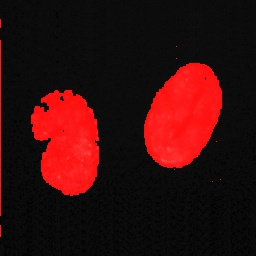
\includegraphics[width=0.3\columnwidth]{mymanualtuning/image3/1_10_800.jpg}
		\label{fig:3graymytune5}
	}
	\subfigure[$\mu=1$, $\alpha=20$, $\lambda_1=150$]
	{
		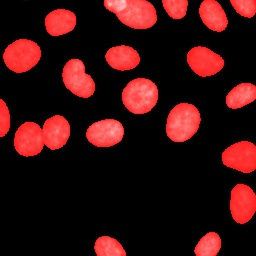
\includegraphics[width=0.3\columnwidth]{mymanualtuning/image3/1_20_150.jpg}
		\label{fig:3graymytune6}
	}
	\subfigure[$\mu=1$, $\alpha=30$, $\lambda_1=150$]
	{
		\includegraphics[width=0.3\columnwidth]{mymanualtuning/image3/1_30_150.jpg}
		\label{fig:3graymytune7}
	}
	\subfigure[$\mu=1$, $\alpha=40$, $\lambda_1=150$]
	{
		\includegraphics[width=0.3\columnwidth]{mymanualtuning/image3/1_40_150.jpg}
		\label{fig:3graymytune8}
	}
%	\subfigure[$\mu=1$, $\alpha=50$, $\lambda_1=150$]
%	{
%		\includegraphics[width=0.3\columnwidth]{mymanualtuning/image3/1_50_150.jpg}
%		\label{fig:3graymytune9}
%	}
	\caption{Segmented output for various combination of $\alpha$ and $\lambda_1$ for Image 3 in the sample set.}
	\label{fig:image3mytune}
\end{figure}

\begin{figure}[!t]
	\centering
	\subfigure[Otsu]
	{
		\includegraphics[width=0.3\columnwidth]{mymanualtuning/image4/otsu_init.jpg}
		\label{fig:4grayotsu}
	}
	\subfigure[K-means ($k=2$)]
	{
		\includegraphics[width=0.3\columnwidth]{mymanualtuning/image4/kmeans_init.jpg}
		\label{fig:4graykmeans}
	}
	\subfigure[EMGMM ($k=2$)]
	{
		\includegraphics[width=0.3\columnwidth]{mymanualtuning/image4/emgmm_init.jpg}
		\label{fig:4grayemgmm}
	}
	\caption{Image 4 from sample set \Cref{fig:sampleset} initial masks.}
	\label{fig:image4init}
\end{figure}

\begin{figure}[!t]
	\centering
	\subfigure[$\mu=1$, $\alpha=30$, $\lambda_1=50$]
	{
		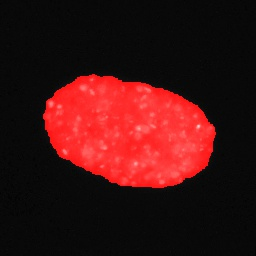
\includegraphics[width=0.3\columnwidth]{mymanualtuning/image4/1_30_50.jpg}
		\label{fig:4graymytune1}
	}
	\subfigure[$\mu=1$, $\alpha=30$, $\lambda_1=100$]
	{
		\includegraphics[width=0.3\columnwidth]{mymanualtuning/image4/1_30_100.jpg}
		\label{fig:4graymytune2}
	}
	\subfigure[$\mu=1$, $\alpha=30$, $\lambda_1=150$]
	{
		\includegraphics[width=0.3\columnwidth]{mymanualtuning/image4/1_30_150.jpg}
		\label{fig:4graymytune3}
	}
	\subfigure[$\mu=1$, $\alpha=40$, $\lambda_1=100$]
	{
		\includegraphics[width=0.3\columnwidth]{mymanualtuning/image4/1_40_100.jpg}
		\label{fig:4graymytune4}
	}
	\subfigure[$\mu=1$, $\alpha=40$, $\lambda_1=150$]
	{
		\includegraphics[width=0.3\columnwidth]{mymanualtuning/image4/1_40_150.jpg}
		\label{fig:4graymytune5}
	}
	\subfigure[$\mu=1$, $\alpha=50$, $\lambda_1=150$]
	{
		\includegraphics[width=0.3\columnwidth]{mymanualtuning/image4/1_50_150.jpg}
		\label{fig:4graymytune6}
	}
	\caption{Segmented output for various combination of $\alpha$ and $\lambda_1$ for Image 4 in the sample set.}
	\label{fig:image4mytune}
\end{figure}

\begin{figure}[!t]
	\centering
	\subfigure[Otsu]
	{
		\includegraphics[width=0.3\columnwidth]{mymanualtuning/image5/otsu_init.jpg}
		\label{fig:5grayotsu}
	}
	\subfigure[K-means ($k=2$)]
	{
		\includegraphics[width=0.3\columnwidth]{mymanualtuning/image5/kmeans_init.jpg}
		\label{fig:5graykmeans}
	}
	\subfigure[EMGMM ($k=2$)]
	{
		\includegraphics[width=0.3\columnwidth]{mymanualtuning/image5/emgmm_init.jpg}
		\label{fig:5grayemgmm}
	}
	\caption{Image 5 from sample set \Cref{fig:sampleset} initial masks.}
	\label{fig:image5init}
\end{figure}

\begin{figure}[!t]
	\centering
	\subfigure[$\mu=1$, $\alpha=30$, $\lambda_1=50$]
	{
		\includegraphics[width=0.3\columnwidth]{mymanualtuning/image5/1_30_50.jpg}
		\label{fig:5graymytune1}
	}
	\subfigure[$\mu=1$, $\alpha=30$, $\lambda_1=100$]
	{
		\includegraphics[width=0.3\columnwidth]{mymanualtuning/image5/1_30_100.jpg}
		\label{fig:5graymytune2}
	}
	\subfigure[$\mu=1$, $\alpha=30$, $\lambda_1=150$]
	{
		\includegraphics[width=0.3\columnwidth]{mymanualtuning/image5/1_30_150.jpg}
		\label{fig:5graymytune3}
	}
	\subfigure[$\mu=1$, $\alpha=40$, $\lambda_1=150$]
	{
		\includegraphics[width=0.3\columnwidth]{mymanualtuning/image5/1_40_100.png}
		\label{fig:5graymytune4}
	}
	\subfigure[$\mu=1$, $\alpha=40$, $\lambda_1=150$]
	{
		\includegraphics[width=0.3\columnwidth]{mymanualtuning/image5/1_40_150.jpg}
		\label{fig:5graymytune5}
	}
	\subfigure[$\mu=1$, $\alpha=50$, $\lambda_1=150$]
	{
		\includegraphics[width=0.3\columnwidth]{mymanualtuning/image5/1_50_150.jpg}
		\label{fig:5graymytune6}
	}
	\caption{Segmented output for various combination of $\alpha$ and $\lambda_1$ for Image 5 in the sample set.}
	\label{fig:image5mytune}
\end{figure}

\begin{figure}[!t]
	\centering
	\subfigure[Otsu]
	{
		\includegraphics[width=0.3\columnwidth]{mymanualtuning/image6/otsu_init.jpg}
		\label{fig:6grayotsu}
	}
	\subfigure[K-means ($k=2$)]
	{
		\includegraphics[width=0.3\columnwidth]{mymanualtuning/image6/kmeans_init.jpg}
		\label{fig:6graykmeans}
	}
	\subfigure[EMGMM ($k=2$)]
	{
		\includegraphics[width=0.3\columnwidth]{mymanualtuning/image6/emgmm_init.jpg}
		\label{fig:6grayemgmm}
	}
	\caption{Image 6 from sample set \Cref{fig:sampleset} initial masks.}
	\label{fig:image6init}
\end{figure}

\begin{figure}[!t]
	\centering
	\subfigure[$\mu=1$, $\alpha=20$, $\lambda_1=20$]
	{
		\includegraphics[width=0.3\columnwidth]{mymanualtuning/image6/1_20_20.jpg}
		\label{fig:6graymytune1}
	}
%	\subfigure[$\mu=1$, $\alpha=20$, $\lambda_1=50$]
%	{
%		\includegraphics[width=0.3\columnwidth]{mymanualtuning/image6/1_20_50.jpg}
%		\label{fig:6graymytune2}
%	}
	\subfigure[$\mu=1$, $\alpha=20$, $\lambda_1=150$]
	{
		\includegraphics[width=0.3\columnwidth]{mymanualtuning/image6/1_20_150.jpg}
		\label{fig:6graymytune2}
	}
	\subfigure[$\mu=1$, $\alpha=30$, $\lambda_1=150$]
	{
		\includegraphics[width=0.3\columnwidth]{mymanualtuning/image6/1_30_150.jpg}
		\label{fig:6graymytune3}
	}
	\subfigure[$\mu=1$, $\alpha=40$, $\lambda_1=50$]
	{
		\includegraphics[width=0.3\columnwidth]{mymanualtuning/image6/1_40_50.jpg}
		\label{fig:6graymytune4}
	}
	\subfigure[$\mu=1$, $\alpha=40$, $\lambda_1=150$]
	{
		\includegraphics[width=0.3\columnwidth]{mymanualtuning/image6/1_40_150.jpg}
		\label{fig:6graymytune5}
	}
	\subfigure[$\mu=1$, $\alpha=50$, $\lambda_1=150$]
	{
		\includegraphics[width=0.3\columnwidth]{mymanualtuning/image6/1_50_150.jpg}
		\label{fig:6graymytune6}
	}
	\caption{Segmented output for various combination of $\alpha$ and $\lambda_1$ for Image 6 in the sample set.}
	\label{fig:image6mytune}
\end{figure}

\end{definition}

\clearpage

\begin{table}[t!]
	\centering
	\caption{Initial means and standard deviations for all images in the sample set for Otsu, K-means and EMGMM clustering.}
	\begin{tabular}{|c|c|c|c|c|}
	\hline
	& $c_0$ & $c_1$ & $s_0$ & $s_1$\\
	\hline
	Image 1 & & & & \\
	\hline
	Otsu & $0.0307515$ & $0.26466$ & $0.0385001$ & $0,0803506$ \\
	\hline
	K-means($k=2$) & $0.0308984$ & $0.267192$ & $0.0387009$ & $0.0793621$ \\
	\hline
	EMGMM ($k=2$) & $0.0305648$ & $0.261392$ & $0.0382529$ & $0.081608$ \\
	\hline
	Image 2 & & & & \\
	\hline
	Otsu & $0.0293218$ & $0.373293$ & $0.054652$ & $0.124376$ \\
	\hline
	K-means($k=2$) & $0.0293218$ & $0.373293$ & $0.054652$ & $0.124376$ \\
	\hline
	EMGMM ($k=2$) & $0.010789$ & $0.321058$ & $0.0211362$ & $0.140498$ \\
	\hline
	Image 3 & & & & \\
	\hline
	Otsu & $0.0422978$ & $0.105043$ & $0.0104066$ & $0.0269333$ \\
	\hline
	K-means($k=2$) & $0.0422978$ & $0.105043$ & $0.0104066$ & $0.0269333$ \\
	\hline
	EMGMM ($k=2$) & $0.042026$ & $0.103124$ & $0.0100784$ & $0.0273395$ \\
	\hline
	Image 4 & & & & \\
	\hline
	Otsu & $0.0424602$ & $0.147303$ & $0.0133024$ & $0.0513289$ \\
	\hline
	K-means($k=2$) & $0.0420671$ & $0.145145$ & $0.0125633$ & $0.0513602$ \\
	\hline
	EMGMM ($k=2$) & $0.0407566$ & $0.136167$ & $0.0102742$ & $0.052472$ \\
	\hline
	Image 5 & & & & \\
	\hline
	Otsu & $0.037086$ & $0.216513$ & $0.0138978$ & $0.0626164$ \\
	\hline
	K-means($k=2$) & $-$ & $-$ & $-$ & $-$ \\
	\hline
	EMGMM ($k=2$) & $0.0343141$ & $0.190501$ & $0.00456055$ & $0.0782783$ \\
	\hline
	Image 6 & & & & \\
	\hline
	Otsu & $0.270483$ & $0.00657006$ & $0.0228327$ & $0.0916426$ \\
	\hline
	K-means($k=2$) & $0.270483$ & $0.00657006$ & $0.0228327$ & $0.0916426$ \\
	\hline
	EMGMM ($k=2$) & $0$ & $0.187883$ & $0$ & $0.133022$ \\
	\hline
\end{tabular}
\label{tab:initmaskvalues}
\end{table}

The final values for the segmentation results are shown in \Cref{tab:manualresults}. The table shows for each image, given the values for the input parameters, whether the degree of acceptance of the output. We take the  final results are the means of object and the background. From the final results, we calculate the values for $p_e$, \Cref{eq:pe}, and $h$ ,\Cref{eq:h}. The means for each image can vary greatly. To put the values of $p_e$ and $h$ into a relative perspective, they are also shown as a fraction of the distance between $c_0$ and $c_1$. Let $k_p \in (0,1)$ be the fraction of the distance $p_e-c_0$ and $c_1-c_0$ as illustrated in \Cref{fig:kp}. Let $k_h \in (k_h,1)$ be the fraction of the distance $h-c_0$ and $c_1-c_0$ as illustrated in \Cref{fig:kh}. The following relation holds $0 < k_p < k_h$.

\begin{figure}[!h]
	\centering
	\begin{tikzpicture}[scale=1]
	\draw[-] (0,0) -- (15,0) node[right] {$p$};
	\draw[shift={(3,0)}] (0pt,4pt) -- (0pt,-4pt) node[below] {$c_0$};
	\draw[shift={(12,0)}] (0pt,4pt) -- (0pt,-4pt) node[below] {$c_1$};
	
	\draw[dashed,black] (5.0,1.5) -- (5.0,-0.3) node[below] {$p_e$};
	
	\draw[black,*-*,thick] (5.0,0.5) -- (4.0,0.5) node[above] {$k_p(c_1-c_0)$} -- (3.0,0.5);
	
	\end{tikzpicture}
	\caption{$p_e$ as a fraction of the distance between $c_0$ and $c_1$.}
	\label{fig:kp}
\end{figure}

\begin{figure}[!h]
	\centering
	\begin{tikzpicture}[scale=1]
	\draw[-] (0,0) -- (15,0) node[right] {$p$};
	\draw[shift={(3,0)}] (0pt,4pt) -- (0pt,-4pt) node[below] {$c_0$};
	\draw[shift={(12,0)}] (0pt,4pt) -- (0pt,-4pt) node[below] {$c_1$};
	
	\draw[dashed,black] (9.0,1.5) -- (9.0,-0.3) node[below] {$h$};
	
	\draw[black,*-*,thick] (9.0,0.5) -- (6.0,0.5) node[above] {$k_h(c_1-c_0)$} -- (3.0,0.5);
	\draw[black,*-*,thick] (9.0,0.5) -- (10.5,0.5) node[above] {$(1-k_h)(c_1-c_0)$} -- (12.0,0.5);
	\end{tikzpicture}
	\caption{$h$ as a fraction of the distance between $c_0$ and $c_1$.}
	\label{fig:kh}
\end{figure}

\begin{center}
	\begin{longtable}{|c|c|c|c|c|c|c|c|c|}
	\caption{Results from manual tuning.} \label{tab:manualresults}\\
	\hline 
	Image & $\alpha$ & $\lambda_1$ & $c_0$ & $c_1$ & $p_e$ & $h$ & $k_p$ & $k_h$ \\ 	
	\hline \rowcolor{bad} 1-O &	30 &	100 &	0.009171 &	0.117209 &	0.025851 &	0.058086 &	0.154387 &	0.452755 \\
	\hline 1-O &	40 &	100	&	0.006909 &	0.110953 &	0.021114 &	0.049359 &	0.136527 &	0.407996 \\
	\hline 1-O &	40 &	50	&	0.006803 &	0.110618 &	0.020976 &	0.065665 &	0.136527 &	0.566987 \\
	\hline \rowcolor{acceptable} 1-O &	40 & 	150	&	0.006953 &	0.111119 &	0.021175 &	0.042396 &	0.136527 &	0.340248 \\
	\hline \rowcolor{acceptable} 1-O &	40 &	200 &	0.007093 &	0.111541 &	0.021353 &	0.038508 &	0.136527 &	0.300772 \\
	\hline \rowcolor{acceptable} 1-O &	45 &	150 &	0.006832 &	0.110758 &	0.020314 &	0.040326 &	0.129732 &	0.322287 \\
	\hline \rowcolor{acceptable} 1-O &	50 &	150 &	0.006681 &	0.110301 &	0.019519 &	0.038516 &	0.123899 &	0.307235 \\
	\hline \rowcolor{bad} 1-K &	30 &	100 &	0.009557 &	0.118306 &	0.026346 &	0.058499 &	0.154387 &	0.450049 \\
	\hline \rowcolor{acceptable} 1-K &	40 &	100 &	0.006928 &	0.111013 &	0.021138 &	0.049379 &	0.136527 &	0.407847 \\
	\hline 1-K &	40 &	50  &	0.006818 &	0.110658 &	0.020995 &	0.065680 &	0.136527 &	0.566856 \\
	\hline \rowcolor{acceptable} 1-K &	40 &	150 &	0.007063 &	0.111430 &	0.021312 &	0.042514 &	0.136527 &	0.339679 \\
	\hline \rowcolor{acceptable} 1-K &	40 &	200 &	0.007176 &	0.111789 &	0.021459 &	0.038600 &	0.136527 &	0.300384 \\
	\hline \rowcolor{acceptable} 1-K &	45 &	150 &	0.006852 &	0.110824 &	0.020340 &	0.040348 &	0.129732 &	0.322165 \\
	\hline \rowcolor{acceptable} 1-K &	50 &	150 &	0.006685 &	0.110311 &	0.019524 &	0.038521 &	0.123899 &	0.307219 \\
	\hline \rowcolor{bad} 1-E &	30 &	150 &	0.008876 &	0.116478 &	0.025489 &	0.049694 &	0.154387 &	0.379343 \\
	\hline \rowcolor{acceptable} 1-E &	40 &	100 &	0.006687 &	0.110890 &	0.020913 &	0.049142 &	0.136527 &	0.407426 \\
	\hline 1-E &	40 &	50  &	0.006788 &	0.110583 &	0.020959 &	0.065649 &	0.136527 &	0.567093 \\
	\hline \rowcolor{acceptable} 1-E &	40 &	150 &	0.006944 &	0.111087 &	0.021163 &	0.042385 &	0.136527 &	0.340313 \\
	\hline \rowcolor{acceptable} 1-E &	40 &	200 &	0.007058 &	0.111434 &	0.021308 &	0.038469 &	0.136527 &	0.300940 \\
	\hline 1-E &	45 &	150 &	0.006800 &	0.110654 &	0.020273 &	0.040291 &	0.129732 &	0.322481 \\
	\hline \rowcolor{acceptable} 1-E &	50 &	150 &	0.006676 &	0.110283 &	0.019512 &	0.038510 &	0.123899 &	0.307268 \\	
	\hline 2-O &	30 &	150 &	0.007640 &	0.309246 &	0.054204 &	0.066628 &	0.154387 &	0.195579 \\
	\hline 2-O &	40 &	50	&	0.007449 &	0.308057 &	0.048489 &	0.076410 &	0.136527 &	0.229407 \\
	\hline 2-O &	40 &	100	&	0.007428 &	0.307890 &	0.048449 &	0.063950 &	0.136527 &	0.188118 \\
	\hline 2-O &	40 &	150	& 	0.007424 &	0.307975 &	0.048457 &	0.059239 &	0.136527 &	0.172400 \\
	\hline 2-O &	40 &	200	&	0.007441 &	0.308094 &	0.048488 &	0.056764 &	0.136527 &	0.164052 \\
	\hline 2-O &	45 &	150	&	0.007423 &	0.307976 &	0.046415 &	0.056577 &	0.129732 &	0.163545 \\
	\hline 2-O &	50 &	150	&	0.007297 &	0.307166 &	0.044450 &	0.054107 &	0.123899 &	0.156103 \\
	\hline 2-K &	30 &	150	&	0.007640 &	0.309246 &	0.054204 &	0.066628 &	0.154387 &	0.195579 \\
	\hline 2-K &	40 &	50	&	0.007449 &	0.308057 &	0.048489 &	0.076410 &	0.136527 &	0.229407 \\
	\hline 2-K &	40 &	100	&	0.007428 &	0.307890 &	0.048449 &	0.063950 &	0.136527 &	0.188118 \\
	\hline 2-K &	40 &	150	&	0.007424 &	0.307975 &	0.048457 &	0.059239 &	0.136527 &	0.172400 \\
	\hline 2-K &	40 &	200	&	0.007441 &	0.308094 &	0.048488 &	0.056764 &	0.136527 &	0.164052 \\
	\hline 2-K &	45 &	150	&	0.007423 &	0.307976 &	0.046415 &	0.056577 &	0.129732 &	0.163545 \\
	\hline 2-K &	50 &	150	&	0.007297 &	0.307166 &	0.044450 &	0.054107 &	0.123899 &	0.156103 \\
	\hline 2-E &	30 &	150	&	0.007556 &	0.308779 &	0.054061 &	0.066498 &	0.154387 &	0.195674 \\
	\hline 2-E &	40 &	50	&	0.007568 &	0.308796 &	0.048694 &	0.076578 &	0.136527 &	0.229095 \\
	\hline 2-E &	40 &	100	&	0.007564 &	0.308815 &	0.048693 &	0.064163 &	0.136527 &	0.187881 \\
	\hline 2-E &	40 &	150	&	0.007566 &	0.308838 &	0.048697 &	0.059458 &	0.136527 &	0.172244 \\
	\hline 2-E &	40 &	200	&	0.007558 &	0.308800 &	0.048686 &	0.056948 &	0.136527 &	0.163952 \\
	\hline 2-E &	45 &	150	&	0.007467 &	0.308260 &	0.046489 &	0.056646 &	0.129732 &	0.163496 \\
	\hline 2-E &	50 &	150	&	0.007343 &	0.307470 &	0.044528 &	0.054178 &	0.123899 &	0.156053 \\
	\hline 3-O &	10 &	150	&	0.041366 &	0.096327 &	0.054571 &	0.108955 &	0.240253 &	1.229755 \\
	\hline 3-O &	10 &	200	&	0.041364 &	0.096323 &	0.054568 &	0.099806 &	0.240253 &	1.063370 \\
	\hline 3-O &	10 &	400	&	0.041359 &	0.096339 &	0.054568 &	0.082894 &	0.240253 &	0.755457 \\
	\hline \rowcolor{bad} 3-O &	10 &	800	&	0.041371 &	0.096708 &	0.054666 &	0.071643 &	0.240253 &	0.547049 \\
	\hline 3-O &	20 &	150	&	0.041323 &	0.095848 &	0.051287 &	0.089056 &	0.182743 &	0.875426 \\
	\hline 3-O &	30 &	150	&	0.041267 &	0.094999 &	0.049563 &	0.080313 &	0.154387 &	0.726674 \\
	\hline \rowcolor{bad} 3-O &	40 &	150	&	0.044802 &	0.057616 &	0.046551 &	0.078701 &	0.136527 &	2.645434 \\
	\hline 3-K &	10 &	150	&	0.041366 &	0.096327 &	0.054571 &	0.108955 &	0.240253 &	1.229755 \\
	\hline 3-K &	10 &	200	&	0.041364 &	0.096323 &	0.054568 &	0.099806 &	0.240253 &	1.063370 \\
	\hline 3-K &	10 &	400	&	0.041359 &	0.096339 &	0.054568 &	0.082894 &	0.240253 &	0.755457 \\
	\hline \rowcolor{bad} 3-K &	10 &	800	&	0.041371 &	0.096708 &	0.054666 &	0.071643 &	0.240253 &	0.547049 \\
	\hline 3-K &	20 &	150	&	0.041323 &	0.095848 &	0.051287 &	0.089056 &	0.182744 &	0.875426 \\
	\hline 3-K &	30 &	150	&	0.041267 &	0.094999 &	0.049563 &	0.080313 &	0.154387 &	0.726674 \\
	\hline \rowcolor{bad} 3-K &	40 &	150	&	0.044802 &	0.057616 &	0.046551 &	0.078701 &	0.136527 &	2.645434 \\
	\hline 3-E &	10 &	150	&	0.041362 &	0.096283 &	0.054557 &	0.108952 &	0.240253 &	1.230667 \\
	\hline 3-E &	10 &	200	&	0.041357 &	0.096260 &	0.054548 &	0.099799 &	0.240253 &	1.064463 \\
	\hline 3-E &	10 &	400	&	0.041356 &	0.096309 &	0.054559 &	0.082890 &	0.240253 &	0.755812 \\
	\hline \rowcolor{bad} 3-E &	10 &	800	&	0.041367 &	0.096932 &	0.054717 &	0.071656 &	0.240253 &	0.545117 \\
	\hline 3-E &	20 &	150	&	0.041321 &	0.095836 &	0.051284 &	0.089054 &	0.182744 &	0.875599 \\
	\hline 3-E &	30 &	150	&	0.041262 &	0.094923 &	0.049545 &	0.080307 &	0.154387 &	0.727635 \\
	\hline \rowcolor{bad} 3-E &	40 &	150	&	0.044849 &	0.057396 &	0.046562 &	0.078753 &	0.136527 &	2.702195 \\
	\hline 4-O &	30 &	50	&	0.040339 &	0.131121 &	0.054355 &	0.107943 &	0.154387 &	0.744683 \\
	\hline 4-O &	30 &	100	&	0.040328 &	0.131038 &	0.054332 &	0.088659 &	0.154387 &	0.532819 \\
	\hline 4-O &	30 &	150	&	0.040319 &	0.130976 &	0.054315 &	0.080354 &	0.154387 &	0.441615 \\
	\hline 4-O &	40 &	100	&	0.040240 &	0.129694 &	0.052453 &	0.082233 &	0.136527 &	0.469438 \\
	\hline 4-O &	40 &	150	&	0.040264 &	0.130244 &	0.052549 &	0.075108 &	0.136527 &	0.387237 \\
	\hline \rowcolor{acceptable} 4-O &	50 &	150	&	0.040232 &	0.129761 &	0.051324 &	0.071509 &	0.123899 &	0.349362 \\
	\hline 4-K &	30 &	50	&	0.040356 &	0.131362 &	0.054406 &	0.107962 &	0.154387 &	0.742875 \\
	\hline 4-K &	30 &	100	&	0.040343 &	0.131304 &	0.054386 &	0.088682 &	0.154387 &	0.531430 \\
	\hline 4-K &	30 &	150	&	0.040339 &	0.131307 &	0.054383 &	0.080387 &	0.154387 &	0.440244 \\
	\hline 4-K &	40 &	100	&	0.040233 &	0.129556 &	0.052428 &	0.082222 &	0.136527 &	0.470084 \\
	\hline 4-K &	40 &	150	&	0.040260 &	0.130177 &	0.052536 &	0.075101 &	0.136527 &	0.387482 \\
	\hline \rowcolor{acceptable} 4-K &	50 &	150	&	0.040223 &	0.129553 &	0.051291 &	0.071494 &	0.123899 &	0.350061 \\
	\hline 4-E &	30 &	50	&	0.040262 &	0.129873 &	0.054097 &	0.107852 &	0.154387 &	0.754261 \\
	\hline 4-E &	30 &	100	&	0.040254 &	0.129884 &	0.054091 &	0.088555 &	0.154387 &	0.538901 \\
	\hline 4-E &	30 &	150	&	0.040237 &	0.129708 &	0.054049 &	0.080225 &	0.154387 &	0.446937 \\
	\hline 4-E &	40 &	100	&	0.040236 &	0.129624 &	0.052439 &	0.082227 &	0.136527 &	0.469763 \\
	\hline 4-E &	40 &	150	&	0.040225 &	0.129532 &	0.052418 &	0.075043 &	0.136527 &	0.389868 \\
	\hline \rowcolor{acceptable} 4-E &	50 &	150	&	0.040201 &	0.129085 &	0.051213 &	0.071456 &	0.123899 &	0.351638 \\
	\hline 5-O &	30 &	50	&	0.034756 &	0.201631 &	0.060519 &	0.104517 &	0.154387 &	0.418045 \\
	\hline 5-O &	30 &	150	&	0.034757 &	0.201659 &	0.060525 &	0.079633 &	0.154387 &	0.268872 \\
	\hline 5-O &	40 &	150	&	0.034675 &	0.200630 &	0.057333 &	0.073912 &	0.136527 &	0.236429 \\
	\hline 5-O &	50 &	150	&	0.034487 &	0.197806 &	0.054722 &	0.069683 &	0.123899 &	0.215506 \\
	\hline 5-K &	30 &	50	&	0.034756 &	0.201631 &	0.060519 &	0.104517 &	0.154387 &	0.418045 \\
	\hline 5-K &	30 &	150	&	0.034757 &	0.201659 &	0.060525 &	0.079633 &	0.154387 &	0.268872 \\
	\hline 5-K &	40 &	150	&	0.034675 &	0.200630 &	0.057333 &	0.073912 &	0.136527 &	0.236429 \\
	\hline 5-K &	50 &	150	&	0.034487 &	0.197806 &	0.054722 &	0.069683 &	0.123899 &	0.215506 \\
	\hline 5-E &	30 &	50	&	0.034683 &	0.200718 &	0.060316 &	0.104407 &	0.154387 &	0.419937 \\
	\hline 5-E &	30 &	150	&	0.034681 &	0.200701 &	0.060313 &	0.079483 &	0.154387 &	0.269859 \\
	\hline 5-E &	40 &	150	&	0.034582 &	0.199297 &	0.057069 &	0.073726 &	0.136527 &	0.237648 \\
	\hline 5-E &	50 &	150	&	0.034580 &	0.199280 &	0.054986 &	0.069870 &	0.123899 &	0.214269 \\
	\hline 6-O &	20 &	20	&	0.002964 &	0.251959 &	0.048466 &	0.136161 &	0.182744 &	0.534939 \\
	\hline 6-O &	20 &	150	&	0.002932 &	0.251781 &	0.048407 &	0.066168 &	0.182744 &	0.254113 \\
	\hline 6-O &	30 &	50	&	0.001533 &	0.228802 &	0.036620 &	0.074639 &	0.154387 &	0.321672 \\
	\hline 6-O &	30 &	150	&	0.001521 &	0.238690 &	0.038137 &	0.053144 &	0.154387 &	0.217666 \\
	\hline 6-O &	40 &	50	&	0.001817 &	0.242106 &	0.034623 &	0.066509 &	0.136527 &	0.269226 \\
	\hline 6-O &	40 &	150	&	0.001815 &	0.242097 &	0.034619 &	0.047477 &	0.136527 &	0.190034 \\
	\hline 6-O &	50 &	50	&	0.001259 &	0.235130 &	0.030236 &	0.059146 &	0.123899 &	0.247513 \\
	\hline 6-O &	50 &	150	&	0.001239 &	0.234857 &	0.030184 &	0.041921 &	0.123899 &	0.174135 \\
	\hline 6-K &	20 &	20	&	0.002964 &	0.251959 &	0.048466 &	0.136161 &	0.182744 &	0.534939 \\
	\hline 6-K &	20 &	150	&	0.002932 &	0.251781 &	0.048407 &	0.066168 &	0.182744 &	0.254113 \\
	\hline 6-K &	30 &	50	&	0.001533 &	0.228802 &	0.036620 &	0.074639 &	0.154387 &	0.321672 \\
	\hline 6-K &	30 &	150	&	0.001521 &	0.238690 &	0.038137 &	0.053144 &	0.154387 &	0.217666 \\
	\hline 6-K &	40 &	50	&	0.001817 &	0.242106 &	0.034623 &	0.066509 &	0.136527 &	0.269226 \\
	\hline 6-K &	40 &	150	&	0.001814 &	0.242097 &	0.034619 &	0.047476 &	0.136527 &	0.190034 \\
	\hline 6-K &	50 &	50	&	0.001259 &	0.235130 &	0.030236 &	0.059146 &	0.123899 &	0.247513 \\
	\hline 6-K &	50 &	150	&	0.001239 &	0.234857 &	0.030185 &	0.041921 &	0.123899 &	0.174135 \\
	\hline 6-E &	20 &	20	&	0.002643 &	0.249529 &	0.047759 &	0.135753 &	0.182744 &	0.539155 \\
	\hline 6-E &	20 &	150	&	0.002584 &	0.249164 &	0.047645 &	0.065530 &	0.182744 &	0.255277 \\
	\hline 6-E &	30 &	50	&	0.002252 &	0.246370 &	0.039940 &	0.076508 &	0.154387 &	0.304183 \\
	\hline 6-E &	30 &	150	&	0.002246 &	0.246324 &	0.039928 &	0.054615 &	0.154387 &	0.214558 \\
	\hline 6-E &	40 &	50	&	0.001527 &	0.238746 &	0.033914 &	0.066025 &	0.136527 &	0.271893 \\
	\hline 6-E &	40 &	150	&	0.001519 &	0.238667 &	0.033896 &	0.046879 &	0.136527 &	0.191277 \\
	\hline 6-E &	50 &	50	&	0.001655 &	0.240298 &	0.031222 &	0.059817 &	0.123899 &	0.243720 \\
	\hline 6-E &	50 &	150	&	0.001645 &	0.240193 &	0.031201 &	0.042755 &	0.123899 &	0.172337 \\
	\hline
\end{longtable} 
\end{center}

Upon comparing the initial means in \Cref{tab:initmaskvalues} and final means for the acceptable and good segmentation results in \Cref{tab:manualresults}, the values of the initial means are larger. This is dues to over-segmentation produced by Otsu, K-means and EMGMM clustering. A na{\"i}ve approach to shifiting the initial means closer to the final means is to dilate the initial mask. This pushes the boundaries of the contour for the object to accept the lower intensity neighbouring pixels as well as removes these relatively higher values from the background mask.

\textcolor{red}{Dilated table results and final radius for dilation.}
To determine the optimal dilation size, we compare the difference of the mean values for each image in \Cref{tab:manualresults}, for the good segmentation results only. These values are shown in \Cref{tab:meanofmeans}. We use an elliptical element for dilation. The results of the dilation and the difference from the respective final means is shown in \Cref{tab:dilateotsu}, \Cref{tab:dilatekmeans} and \Cref{tab:dilateemgmm} for the initial masks obtained from Otsu binarization, K-means and EMGMM clustering respectively. The closest values to the average final mean is highlighted in blue. From the tables it can be seen that a diation size of 3 for a elliptical dilation element results in mean values that are closest to the average final means.

\begin{table}
	\centering
	\caption{Average of final means for good segmentations.}
	\begin{tabular}{|c|c|c|}
		\hline 
		Image & $\bar{c_0}$ & $\bar{c_1}$ \\ 
		\hline 
		1 & 0,006824 & 0,110693 \\ 
		\hline 
		2 & 0,007468 & 0,308217 \\ 
		\hline 
		3 & 0,041334 & 0,095952 \\ 
		\hline 
		4 & 0,040282 & 0,130360 \\ 
		\hline 
		5 & 0,034656 & 0,200287 \\ 
		\hline 
		6 & 0,001926 & 0,241672 \\ 
		\hline 
	\end{tabular}
	\label{tab:meanofmeans}
\end{table}


\begin{longtable}{|c|c|c|c|c|c|c|}
	\caption{Dilation after Otsu binarization.} \label{tab:dilateotsu}\\
	\hline 
	Image & Size & $c_0$ & $c_1$ & $|c_0-\bar{c_0}|$ & $|c_1-\bar{c_1}|$ & $\sum_i |c_i-\bar{c_i}|$ \\ 
	\hline 1 &	3 &	0.027716 &	0.205161 &	0.020892 &	0.094468 &	0.115360 \\
	\hline 1 &	5 &	0.026188 &	0.173038 &	0.019364 &	0.062345 &	0.081709 \\
	\hline 1 &	7 &	0.024682 &	0.151369 &	0.017858 &	0.040676 &	0.058534 \\
	\hline 1 &	9 &	0.023158 &	0.136273 &	0.016334 &	0.025580 &	0.041914 \\
	\hline 1 &	11 &	0.021564 &	0.124931 &	0.014739 &	0.014238 &	0.028978 \\
	\hline 1 &	13 &	0.019981 &	0.116536 &	0.013157 &	0.005843 &	0.018999 \\
	\hline \rowcolor{closest} 1 &	15 &	0.018341 &	0.109705 &	0.011517 &	0.000988 &	0.012505 \\
	\hline \rowcolor{closest} 2 &	3 &	0.007563 &	0.301761 &	9.47e-05 &	0.006456 &	0.006551 \\
	\hline 2 &	5 &	0.006025 &	0.286271 &	0.001443 &	0.021946 &	0.023389 \\
	\hline 2 &	7 &	0.005386 &	0.273472 &	0.002082 &	0.034745 &	0.036827 \\
	\hline 2 &	9 &	0.004936 &	0.262053 &	0.002532 &	0.046164 &	0.048696 \\
	\hline 2 &	11 &	0.004587 &	0.250695 &	0.002881 &	0.057522 &	0.060403 \\
	\hline 2 &	13 &	0.004277 &	0.240651 &	0.003191 &	0.067566 &	0.070757 \\
	\hline 2 &	15 &	0.004041 &	0.231146 &	0.003428 &	0.077071 &	0.080498 \\
	\hline \rowcolor{closest} 3 &	3 &	0.041796 &	0.090729 &	0.000462 &	0.005223 &	0.005685 \\
	\hline 3 &	5 &	0.041641 &	0.084544 &	0.000307 &	0.011408 &	0.011715 \\
	\hline 3 &	7 &	0.041535 &	0.080118 &	0.000201 &	0.015834 &	0.016034 \\
	\hline 3 &	9 &	0.042983 &	0.076541 &	0.001649 &	0.019411 &	0.021059 \\
	\hline 3 &	11 &	0.041439 &	0.073293 &	0.000105 &	0.022659 &	0.022764 \\
	\hline 3 &	13 &	0.041397 &	0.070676 &	6.27e-05 &	0.025276 &	0.025339 \\
	\hline 3 &	15 &	0.041369 &	0.068354 &	3.48e-05 &	0.027599 &	0.027633 \\
	\hline 4 &	3 &	0.041060 &	0.133918 &	0.000778 &	0.003558 &	0.004336 \\
	\hline \rowcolor{closest} 4 &	5 &	0.040715 &	0.128101 &	0.000433 &	0.002259 &	0.002692 \\
	\hline 4 &	7 &	0.040534 &	0.122898 &	0.000252 &	0.007462 &	0.007714 \\
	\hline 4 &	9 &	0.040429 &	0.118341 &	0.000147 &	0.012019 &	0.012166 \\
	\hline 4 &	11 &	0.040354 &	0.113853 &	7.17e-05 &	0.016507 &	0.016579 \\
	\hline 4 &	13 &	0.040297 &	0.109960 &	1.53e-05 &	0.020400 &	0.020415 \\
	\hline 4 &	15 &	0.040235 &	0.106414 &	4.70e-05 &	0.023946 &	0.023993 \\
	\hline \rowcolor{closest} 5 &	3 &	0.035322 &	0.203137 &	0.000666 &	0.002850 &	0.003516 \\
	\hline 5 &	5 &	0.034726 &	0.193711 &	7.02e-05 &	0.006576 &	0.006646 \\
	\hline 5 &	7 &	0.034434 &	0.184644 &	0.000222 &	0.015643 &	0.015865 \\
	\hline 5 &	9 &	0.034281 &	0.176477 &	0.000375 &	0.023810 &	0.024185 \\
	\hline 5 &	11 &	0.034188 &	0.168599 &	0.000468 &	0.031688 &	0.032156 \\
	\hline 5 &	13 &	0.034120 &	0.161732 &	0.000536 &	0.038555 &	0.039091 \\
	\hline 5 &	15 &	0.034056 &	0.155296 &	0.000600 &	0.044991 &	0.045591 \\
	\hline \rowcolor{closest} 6 &	3 &	0.000457 &	0.209125 &	0.001469 &	0.032547 &	0.034016 \\
	\hline 6 &	5 &	7.29e-05 &	0.171123 &	0.001853 &	0.070549 &	0.072402 \\
	\hline 6 &	7 &	1.84e-05 &	0.144280 &	0.001908 &	0.097392 &	0.099299 \\
	\hline 6 &	9 &	1.08e-05 &	0.125501 &	0.001915 &	0.116171 &	0.118086 \\
	\hline 6 &	11 &	1.15e-05 &	0.110706 &	0.001914 &	0.130966 &	0.132880 \\
	\hline 6 &	13 &	1.27e-05 &	0.100486 &	0.001913 &	0.141186 &	0.143099 \\
	\hline 6 &	15 &	1.44e-05 &	0.092725 &	0.001912 &	0.148947 &	0.150858 \\
	\hline 
\end{longtable} 

\begin{longtable}{|c|c|c|c|c|c|c|}
	\caption{Dilation after K-means clustering.} \label{tab:dilatekmeans}\\
	\hline
	Image & Size & $c_0$ & $c_1$ & $|c_0-\bar{c_0}|$ & $|c_1-\bar{c_1}|$ & $\sum_i |c_i-\bar{c_i}|$ \\ 
	\hline 1 &	3 &	0.027716 &	0.205161 &	0.020892 &	0.094468 &	0.115360 \\
	\hline 1 &	5 &	0.026188 &	0.173038 &	0.019364 &	0.062345 &	0.081709 \\
	\hline 1 &	7 &	0.024682 &	0.151369 &	0.017858 &	0.040676 &	0.058534 \\
	\hline 1 &	9 &	0.023158 &	0.136273 &	0.016334 &	0.025580 &	0.041914 \\
	\hline 1 &	11 &	0.021564 &	0.124931 &	0.014739 &	0.014238 &	0.028978 \\
	\hline 1 &	13 &	0.019981 &	0.116536 &	0.013157 &	0.005843 &	0.018999 \\
	\hline \rowcolor{closest} 1 &	15 &	0.018341 &	0.109705 &	0.011517 &	0.000988 &	0.012505 \\
	\hline \rowcolor{closest} 2 &	3 &	0.007563 &	0.301761 &	9.47e-05 &	0.006456 &	0.006551 \\
	\hline 2 &	5 &	0.006025 &	0.286271 &	0.001443 &	0.021946 &	0.023389 \\
	\hline 2 &	7 &	0.005386 &	0.273472 &	0.002082 &	0.034745 &	0.036827 \\
	\hline 2 &	9 &	0.004936 &	0.262053 &	0.002532 &	0.046164 &	0.048696 \\
	\hline 2 &	11 &	0.004587 &	0.250695 &	0.002881 &	0.057522 &	0.060403 \\
	\hline 2 &	13 &	0.004277 &	0.240651 &	0.003191 &	0.067566 &	0.070757 \\
	\hline 2 &	15 &	0.004041 &	0.231146 &	0.003427 &	0.077071 &	0.080499 \\
	\hline \rowcolor{closest} 3 &	3 &	0.041796 &	0.090729 &	0.000462 &	0.005223 &	0.005685 \\
	\hline 3 &	5 &	0.041641 &	0.084544 &	0.000307 &	0.011408 &	0.011715 \\
	\hline 3 &	7 &	0.041535 &	0.080118 &	0.000201 &	0.015834 &	0.016034 \\
	\hline 3 &	9 &	0.041480 &	0.076541 &	0.000146 &	0.019411 &	0.019557 \\
	\hline 3 &	11 &	0.041439 &	0.073293 &	0.000105 &	0.022659 &	0.022764 \\
	\hline 3 &	13 &	0.041397 &	0.070676 &	6.27e-05 &	0.025276 &	0.025339 \\
	\hline 3 &	15 &	0.041369 &	0.068354 &	3.48e-05 &	0.027599 &	0.027633 \\
	\hline \rowcolor{closest} 4 &	3 &	0.041060 &	0.133918 &	0.000778 &	0.003558 &	0.004336 \\
	\hline 4 &	5 &	0.040715 &	0.128101 &	0.000433 &	0.002259 &	0.002692 \\
	\hline 4 &	7 &	0.040534 &	0.122898 &	0.000252 &	0.007462 &	0.007714 \\
	\hline 4 &	9 &	0.040429 &	0.118341 &	0.000147 &	0.012019 &	0.012166 \\
	\hline 4 &	11 &	0.040354 &	0.113853 &	7.17e-05 &	0.016507 &	0.016579 \\
	\hline 4 &	13 &	0.040297 &	0.109960 &	1.53e-05 &	0.020400 &	0.020415 \\
	\hline 4 &	15 &	0.040235 &	0.106414 &	4.70e-05 &	0.023946 &	0.023993 \\
	\hline \rowcolor{closest} 5 &	3 &	0.035322 &	0.203137 &	0.000666 &	0.002850 &	0.003516 \\
	\hline 5 &	5 &	0.034726 &	0.193711 &	7.02e-05 &	0.006576 &	0.006646 \\
	\hline 5 &	7 &	0.034434 &	0.184644 &	0.000222 &	0.015643 &	0.015865 \\
	\hline 5 &	9 &	0.034281 &	0.176477 &	0.000375 &	0.023810 &	0.024185 \\
	\hline 5 &	11 &	0.034188 &	0.168599 &	0.000468 &	0.031688 &	0.032156 \\
	\hline 5 &	13 &	0.034120 &	0.161732 &	0.000536 &	0.038555 &	0.039091 \\
	\hline 5 &	15 &	0.034056 &	0.155296 &	0.000600 &	0.044991 &	0.045591 \\
	\hline \rowcolor{closest} 6 &	3 &	0.000457 &	0.209125 &	0.001469 &	0.032547 &	0.034016 \\
	\hline 6 &	5 &	7.29e-05 &	0.171123 &	0.001853 &	0.070549 &	0.072402 \\
	\hline 6 &	7 &	1.84e-05 &	0.144280 &	0.001908 &	0.097392 &	0.099299 \\
	\hline 6 &	9 &	1.08e-05 &	0.125501 &	0.001915 &	0.116171 &	0.118086 \\
	\hline 6 &	11 &	1.15e-05 &	0.110706 &	0.001914 &	0.130966 &	0.132880 \\
	\hline 6 &	13 &	1.27e-05 &	0.100486 &	0.001913 &	0.141186 &	0.143099 \\
	\hline 6 &	15 &	1.44e-05 &	0.092725 &	0.001912 &	0.148947 &	0.150858 \\
	\hline 
\end{longtable} 

\begin{longtable}{|c|c|c|c|c|c|c|}
	\caption{Dilation after EM-GMM clustering.} \label{tab:dilateemgmm}\\
	\hline
	Image & Size & $c_0$ & $c_1$ & $|c_0-\bar{c_0}|$ & $|c_1-\bar{c_1}|$ & $\sum_i |c_i-\bar{c_i}|$ \\ 
	\hline 1 &	3 &	0.027251 &	0.198511 &	0.020427 &	0.087818 &	0.108245 \\
	\hline 1 &	5 &	0.025597 &	0.166707 &	0.018773 &	0.056014 &	0.074787 \\
	\hline 1 &	7 &	0.023968 &	0.146071 &	0.017144 &	0.035378 &	0.052522 \\
	\hline 1 &	9 &	0.022313 &	0.131983 &	0.015489 &	0.021290 &	0.036779 \\
	\hline 1 &	11 &	0.020595 &	0.121338 &	0.013771 &	0.010645 &	0.024416 \\
	\hline 1 &	13 &	0.018866 &	0.113441 &	0.012042 &	0.002748 &	0.014789 \\
	\hline \rowcolor{closest} 1 &	15 &	0.017084 &	0.107025 &	0.010260 &	0.003668 &	0.013928 \\
	\hline \rowcolor{closest} 2 &	3 &	0.006516 &	0.294763 &	0.000952 &	0.013454 &	0.014406 \\
	\hline 2 &	5 &	0.005719 &	0.280590 &	0.001748 &	0.027627 &	0.029375 \\
	\hline 2 &	7 &	0.005165 &	0.268079 &	0.002303 &	0.040138 &	0.042441 \\
	\hline 2 &	9 &	0.004774 &	0.256867 &	0.002694 &	0.051350 &	0.054044 \\
	\hline 2 &	11 &	0.004438 &	0.245779 &	0.003030 &	0.062438 &	0.065468 \\
	\hline 2 &	13 &	0.004165 &	0.235995 &	0.003303 &	0.072222 &	0.075525 \\
	\hline 2 &	15 &	0.003947 &	0.226736 &	0.003521 &	0.081481 &	0.085002 \\
	\hline \rowcolor{closest} 3 &	3 &	0.041729 &	0.089955 &	0.000395 &	0.005997 &	0.006392 \\
	\hline 3 &	5 &	0.041603 &	0.083968 &	0.000269 &	0.011984 &	0.012252 \\
	\hline 3 &	7 &	0.041502 &	0.079529 &	0.000168 &	0.016423 &	0.016590 \\
	\hline 3 &	9 &	0.041435 &	0.075914 &	0.000101 &	0.020038 &	0.020138 \\
	\hline 3 &	11 &	0.041384 &	0.072717 &	5.00e-05 &	0.023236 &	0.023285 \\
	\hline 3 &	13 &	0.041335 &	0.070134 &	1.30e-06 &	0.025819 &	0.025819 \\
	\hline 3 &	15 &	0.041299 &	0.067855 &	3.52e-05 &	0.028097 &	0.028132 \\
	\hline \rowcolor{closest} 4 &	3 &	0.040788 &	0.114645 &	0.000506 &	0.015715 &	0.016221 \\
	\hline 4 &	5 &	0.040886 &	0.099155 &	0.000604 &	0.031205 &	0.031809 \\
	\hline 4 &	7 &	0.041119 &	0.087943 &	0.000838 &	0.042417 &	0.043255 \\
	\hline 4 &	9 &	0.041369 &	0.080176 &	0.001087 &	0.050184 &	0.051271 \\
	\hline 4 &	11 &	0.041665 &	0.074350 &	0.001383 &	0.056010 &	0.057393 \\
	\hline 4 &	13 &	0.042029 &	0.070365 &	0.001747 &	0.059995 &	0.061742 \\
	\hline 4 &	15 &	0.042324 &	0.067586 &	0.002042 &	0.062774 &	0.064816 \\
	\hline \rowcolor{closest} 5 &	3 &	0.034368 &	0.147707 &	0.000288 &	0.052580 &	0.052868 \\
	\hline 5 &	5 &	0.034298 &	0.119630 &	0.000358 &	0.080657 &	0.081015 \\
	\hline 5 &	7 &	0.034222 &	0.102563 &	0.000434 &	0.097724 &	0.098158 \\
	\hline 5 &	9 &	0.034181 &	0.092259 &	0.000475 &	0.108028 &	0.108504 \\
	\hline 5 &	11 &	0.034143 &	0.085251 &	0.000513 &	0.115036 &	0.115549 \\
	\hline 5 &	13 &	0.034105 &	0.080911 &	0.000551 &	0.119377 &	0.119928 \\
	\hline 5 &	15 &	0.034075 &	0.077899 &	0.000581 &	0.122388 &	0.122969 \\
	\hline \rowcolor{closest} 6 &	3 &	0.000000 &	0.136655 &	0.001926 &	0.105017 &	0.106943 \\
	\hline 6 &	5 &	0.000000 &	0.116893 &	0.001926 &	0.124779 &	0.126705 \\
	\hline 6 &	7 &	0.000000 &	0.103734 &	0.001926 &	0.137938 &	0.139864 \\
	\hline 6 &	9 &	0.000000 &	0.094463 &	0.001926 &	0.147209 &	0.149135 \\
	\hline 6 &	11 &	0.000000 &	0.087325 &	0.001926 &	0.154347 &	0.156273 \\
	\hline 6 &	13 &	0.000000 &	0.082486 &	0.001926 &	0.159186 &	0.161112 \\
	\hline 6 &	15 &	0.000000 &	0.079177 &	0.001926 &	0.162495 &	0.164421 \\
	\hline 
\end{longtable} 


\textcolor{red}{Updated equations taking into account $k_p$ and $k_h$.}
When defining the values for $p_e$ and $h$ implicitely and $k_p$ and $k_h$ respectively, we can find the updated equation for determining $\alpha$ following from \Cref{eq:alphaapproximation}
\begin{equation*}\begin{split}
		\alpha & = \left( \frac{c_1-c_0}{p_e-c_0} -1 \right)^2 \\
		& = \left( \frac{c_1-c_0-p_e+c_0}{p_e-c_0} \right)^2 \\
		& = \left( \frac{c_1-c_0 -c_0-k_p(c_1-c_0)+c_0}{c_0 + k_p(c_1-c_0)-c_0} \right)^2\\
		& = \left( \frac{c_1-c_0-k_p(c_1-c_0)}{k_p(c_1-c_0)} \right)^2\\
		& = \left( \frac{(1-k_p)(c_1-c_0)}{k_p(c_1-c_0)} \right)^2
\end{split}\end{equation*}

Therefore, given $k_p$, the equation to calculate $\alpha$ is
\begin{equation}
	\alpha = \left( \frac{1-k_p}{k_p} \right)^2
	\label{eq:alphafromkp}
\end{equation}

\begin{equation}\begin{split}
	\alpha-1 = \frac{1-2k_p+k_p^2-k_p^2}{k_p^2} = \frac{1-2k_p}{k_p^2}
\end{split}\end{equation}

Following from \Cref{eq:lambda1approximation}...

\begin{equation*}
	h = c_0+k_h(c_1-c_0) = c_1-(1-k_h)(c_1-c_0)
\end{equation*}
\begin{equation*}\begin{split}
	&\alpha (c_0+k_h(c_1-c_0)-c_0)^2-(c_1-(1-k_h)(c_1-c_0)-c_1)^2\\
	=\,& \alpha k_h^2 (c_1-c_0)^2 + (k_h-1)^2(c_1-c_0)^2 \\
	=\,& \alpha k_h^2(c_1-c_0)^2-(k_h-1)^2(c_1-c_0)^2 \\
	=\,& (c_1-c_0)^2(\alpha k_h^2-(k_h-1)^2)\\
	=\,& (c_1-c_0)^2 \left( \alpha k_h^2 - k_h^2 + 2k_h - 1 \right)\\
	=\,& (c_1-c_0)^2 \left( k_h^2(\alpha-1) + 2k_h -1 \right) \\
	=\,& (c_1-c_0)^2\left( \left( \frac{1-2k_p}{k_p^2} \right)k_h^2 +2k_h -1 \right)
\end{split}\end{equation*}

\begin{equation}
	\lambda_1 = \frac{\mu \left( 2\sqrt{2}+4\right)}{(c_1-c_0)^2\left( \left( \frac{1-2k_p}{k_p^2} \right)k_h^2 +2k_h -1 \right)}
	\label{eq:lambda1fromkpandkh}
\end{equation}

\section{Experimental Results}
\label{sec:cvgc_experimentalresults}

\textcolor{red}{Present and analyse the experimental results.} The parameters $\alpha$ and $\lambda_1$, in the proposed parameter estimation method, depend greatly on predicting good final means, $c_0$ and $c_1$, as well as $p_e$ and $h$ for the ideal segmentation. For determining $\alpha$ we find the average of all $k_p$ in \Cref{tab:manualresults} for all good segmentations. This is calculated to be
\begin{equation*}
	k_p = 0.154494.
\end{equation*}
From this we can calculate the value for $\alpha$ immediately using \Cref{eq:alphafromkp}. This turns out to be
\begin{equation}
\alpha = 29.9509.
\end{equation}
Similarly, to determine $h$ we find the average of all $k_h$ in \Cref{tab:manualresults} for all good segmentations. This is calculated to be
\begin{equation*}
	k_h = 0.412737.
\end{equation*}
It is rarely the case where this is known or can be calculated, if ever at all. Instead, we use the results from three popular unsupervised clustering algorithms and compare the final segmented result against a ground truth. The algorithms chosen to generate an initial mask, from which we calculate $c_0$ and $c_1$ are: \textit{Otsu} \citep{Otsu1979}, $k$-means \citep{Kanungo2002} with $k=2$ and Expectation Maximisation Gaussian Mixture Modelling (\textbf{EMGMM}) \citep{Figueiredo2002} with $k=2$. From observations we see that these algorithms tend to generate over-segmented results. In light of this, we generate a fourth mask which is an EMGMM output with dilation. For dilation we used an elliptical shape with a radius of $3px$. Once we have the initial mask and have calculated the initial $c_0$ and $c_1$ from this initial mask, we calculate $\lambda_1$ using \Cref{eq:lambda1fromkpandkh}. Now that we have $\alpha$ and $\lambda_1$ we calculate $\lambda_0$ using \Cref{eq:l0l1dependancy}. We set the termination criterion at $\epsilon=1 \times 10^{-3}$.

We also compare our results  to two previously published parameter settings.
The first is the parameter settings used in \citep{ElZehiry2007}, by El Zehiry \textit{et al.}, which is where this technique was first published. Their results showed excellent segmentation ouptput on synthetic images and mammography images with very high robustness against noise. They do not specify the noise type.
The second parameter setting which we test against is presented in \citep{Maska2013}, by Masaka \textit{et al.}. Their parameter setting where based on a timelapse series of fluorescence images. Their scheme is a hybrid of algorithms design to segmente whole fluorescent cells, however, we use the parameters settings they've presented for segmentation only. Their parameters were obtained by minimising the Jaccard coefficient over the timelapse series. Their results show a greater area of cell detection and smoother boundaries. Although, the smoother contours are a result of CED-ORI [cite cedori] which is part of the scheme before segmentation.

The initial masks used in subsequent parameter estimation is shown in \Cref{fig:test188,fig:test195,fig:test228,fig:test1057,fig:test1265,fig:test10093,fig:test10102,fig:test10104,fig:test12294,fig:test12627,fig:test13432,fig:test13438,fig:test13899,fig:test13901,fig:test21749,fig:test21759,fig:test32140,fig:test35278,fig:test37338,fig:test37339,fig:test38974,fig:test40217,fig:test40968,fig:test41066,fig:test42451}.

The segmented outputs are shown in \Cref{fig:testresult188,fig:testresult195,fig:testresult228,fig:testresult1057,fig:testresult1265,fig:testresult10093,fig:testresult10102,fig:testresult10104,fig:testresult12294,fig:testresult12627,fig:testresult13432,fig:testresult13438,fig:testresult13899,fig:testresult13901,fig:testresult21749,fig:testresult21759,fig:testresult32140,fig:testresult35278,fig:testresult37338,fig:testresult37339,fig:testresult38974,fig:testresult40217,fig:testresult40968,fig:testresult41066,fig:testresult42451}.

The parameter settings and corresponding resutls are summarised in \Cref{tab:segmentationresults}. The last column, labelled \textit{"Diff"}, is a measure of how far off the final means are from the ideal. It is calculated as 
\begin{equation*}
	Diff = |c_{0}^{Final}-c_{0}^{Ideal}| + |c_{1}^{Final}-c_{1}^{Ideal}|.
\end{equation*}

In \Cref{tab:segmentationresults} differentiate between methods on the same image as follows:

\textbf{[imageno]-[method]}, 

where \textit{imageno} goes from $1$ to $25$ and \textit{method} is defined as follows:
\begin{enumerate}
	\item [\textbf{n}] - using parameter setting presented in \citep{ElZehiry2007}.
	\item [\textbf{m}] - using parameter setting presented in \citep{Maska2013}.
	\item [\textbf{o}] - Proposed method with parameters estimated from an initial Otsu segmentation.
	\item [\textbf{k}] - Proposed method with parameters estimated from an initial K-means segmentation with $k=2$.
	\item [\textbf{e}] - Proposed method with parameters estimated from an initial EMGMM segmentation with $k=2$.
	\item [\textbf{d}] - Proposed method with parameters estimated from an initial EMGMM segmentation with $k=2$ and an elliptical dilation of $3px$.
\end{enumerate}

\clearpage
%%%%%%%%%%%%%%%%%%%%%%%%%%%%%%%%%%%%%%%%%%%%%%%%%%%%%%%
% 188
\begin{figure}[!h]
	\centering
	\subfigure[Otsu.]
	{
		\includegraphics[width=0.23\columnwidth]{propsedcv/otsu/otsu188initmask}
		\label{fig:otsu188}
	}
	\subfigure[K-means.]
	{
		\includegraphics[width=0.23\columnwidth]{propsedcv/kmeans/kmeans2188initmask}
		\label{fig:kmeans188}
	}
	\subfigure[EMGMM.]
	{
		\includegraphics[width=0.23\columnwidth]{propsedcv/emgmm/emgmm2188initmask}
		\label{fig:emgmm188}
	}
	\subfigure[EMGMM and dilation.]
	{
		\includegraphics[width=0.23\columnwidth]{propsedcv/dilated/emgmm2188initmask}
		\label{fig:emgmmdilate188}
	}
	\caption{Image 1 from test set \Cref{AppendixA} initial masks.}
	\label{fig:test188}
\end{figure}

\begin{figure}[!h]
	\centering
	\subfigure[$\mu=0.1\times255^2$, $\lambda_0=\lambda_1=1$ .]
	{
		\includegraphics[width=0.315\columnwidth]{propsedcv/def/def188}
		\label{fig:default188}
	}
	\subfigure[$\mu=0.01$, $\lambda_0=85$, $\lambda_1=1$, $c_0=0.005861$, $c_1=0.436831$.]
	{
		\includegraphics[width=0.315\columnwidth]{propsedcv/shapetrack/shapetrack188}
		\label{fig:shapetrack188}
	}
	\subfigure[Proposed with initial Otsu. $\mu=1$, $\alpha=29.9509$, $\lambda_1=7.47524$.]
	{
		\includegraphics[width=0.315\columnwidth]{propsedcv/otsu/otsu188finmask}
		\label{fig:propsedCVotsu188}
	}
	\subfigure[Proposed with initial K-means. $\mu=1$, $\alpha=29.9509$, $\lambda_1=7.47525$.]
	{
		\includegraphics[width=0.315\columnwidth]{propsedcv/kmeans/kmeans2188finmask}
		\label{fig:propsedCVkmeans188}
	}
	\subfigure[Proposed with initial EMGMM. $\mu=1$, $\alpha=29.9509$, $\lambda_1=7.61164$.]
	{
		\includegraphics[width=0.315\columnwidth]{propsedcv/emgmm/emgmm2188finmask}
		\label{fig:propsedCVemgmm188}
	}
	\subfigure[Proposed with initial EMGMM and dilation. $\mu=1$, $\alpha=29.9509$, $\lambda_1=8.17148$.]
	{
		\includegraphics[width=0.315\columnwidth]{propsedcv/dilated/emgmm2188finmask}
		\label{fig:propsedCVemgmmdilate188}
	}
	\caption{Image 1 from test set \Cref{AppendixA} segmentation results.}
	\label{fig:testresult188}
\end{figure}
%%%%%%%%%%%%%%%%%%%%%%%%%%%%%%%%%%%%%%%%%%%%%%%%%%%%%%%
% 195
\begin{figure}[!h]
	\centering
	\subfigure[Otsu.]
	{
		\includegraphics[width=0.23\columnwidth]{propsedcv/otsu/otsu195initmask}
		\label{fig:otsu195}
	}
	\subfigure[K-means.]
	{
		\includegraphics[width=0.23\columnwidth]{propsedcv/kmeans/kmeans2195initmask}
		\label{fig:kmeans195}
	}
	\subfigure[EMGMM.]
	{
		\includegraphics[width=0.23\columnwidth]{propsedcv/emgmm/emgmm2195initmask}
		\label{fig:emgmm195}
	}
	\subfigure[EMGMM and dilation.]
	{
		\includegraphics[width=0.23\columnwidth]{propsedcv/dilated/emgmm2195initmask}
		\label{fig:emgmmdilate195}
	}
	\caption{Image 2 from test set \Cref{AppendixA} initial masks.}
	\label{fig:test195}
\end{figure}

\begin{figure}[!h]
	\centering
	\subfigure[$\mu= 0.1\times255^2$, $\lambda_0=\lambda_1=1$.]
	{
		\includegraphics[width=0.315\columnwidth]{propsedcv/def/def195}
		\label{fig:default195}
	}
	\subfigure[$\mu=0.01$, $\lambda_0=85$, $\lambda_1=1$.]
	{
		\includegraphics[width=0.315\columnwidth]{propsedcv/shapetrack/shapetrack195}
		\label{fig:shapetrack195}
	}
	\subfigure[Proposed with initial Otsu. $\mu=1$, $\alpha=29.9509$, $\lambda_1=139.983$.]
	{
		\includegraphics[width=0.315\columnwidth]{propsedcv/otsu/otsu195finmask}
		\label{fig:propsedCVotsu195}
	}
	\subfigure[Proposed with initial K-means. $\mu=1$, $\alpha=29.9509$, $\lambda_1=139.984$.]
	{
		\includegraphics[width=0.315\columnwidth]{propsedcv/kmeans/kmeans2195finmask}
		\label{fig:propsedCVkmeans195}
	}
	\subfigure[Proposed with initial EMGMM. $\mu=1$, $\alpha=29.9509$, $\lambda_1=148.373$.]
	{
		\includegraphics[width=0.315\columnwidth]{propsedcv/emgmm/emgmm2195finmask}
		\label{fig:propsedCVemgmm195}
	}
	\subfigure[Proposed with initial EMGMM and dilation. $\mu=1$, $\alpha=29.9509$, $\lambda_1=606.199$.]
	{
		\includegraphics[width=0.315\columnwidth]{propsedcv/dilated/emgmm2195finmask}
		\label{fig:propsedCVemgmmdilate195}
	}
	\caption{Image 2 from test set \Cref{AppendixA} segmentation results.}
	\label{fig:testresult195}
\end{figure}
%%%%%%%%%%%%%%%%%%%%%%%%%%%%%%%%%%%%%%%%%%%%%%%%%%%%%%%
% 228
\begin{figure}[!h]
	\centering
	\subfigure[Otsu.]
	{
		\includegraphics[width=0.23\columnwidth]{propsedcv/otsu/otsu228initmask}
		\label{fig:otsu228}
	}
	\subfigure[K-means.]
	{
		\includegraphics[width=0.23\columnwidth]{propsedcv/kmeans/kmeans2228initmask}
		\label{fig:kmeans228}
	}
	\subfigure[EMGMM.]
	{
		\includegraphics[width=0.23\columnwidth]{propsedcv/emgmm/emgmm2228initmask}
		\label{fig:emgmm228}
	}
	\subfigure[EMGMM and dilation.]
	{
		\includegraphics[width=0.23\columnwidth]{propsedcv/dilated/emgmm2228initmask}
		\label{fig:emgmmdilate228}
	}
	\caption{Image 3 from test set \Cref{AppendixA} initial masks.}
	\label{fig:test228}
\end{figure}

\begin{figure}[!h]
	\centering
	\subfigure[$\mu= 0.1\times255^2$, $\lambda_0=\lambda_1=1$.]
	{
		\includegraphics[width=0.315\columnwidth]{propsedcv/def/def228}
		\label{fig:default228}
	}
	\subfigure[$\mu=0.01$, $\lambda_0=85$, $\lambda_1=1$.]
	{
		\includegraphics[width=0.315\columnwidth]{propsedcv/shapetrack/shapetrack228}
		\label{fig:shapetrack228}
	}
	\subfigure[Proposed with initial Otsu. $\mu=1$, $\alpha=29.9509$, $\lambda_1=9.93033
	$.]
	{
		\includegraphics[width=0.315\columnwidth]{propsedcv/otsu/otsu228finmask}
		\label{fig:propsedCVotsu228}
	}
	\subfigure[Proposed with initial K-means. $\mu=1$, $\alpha=29.9509$, $\lambda_1=9.93034$.]
	{
		\includegraphics[width=0.315\columnwidth]{propsedcv/kmeans/kmeans2228finmask}
		\label{fig:propsedCVkmeans228}
	}
	\subfigure[Proposed with initial EMGMM. $\mu=1$, $\alpha=29.9509$, $\lambda_1=14.4226$.]
	{
		\includegraphics[width=0.315\columnwidth]{propsedcv/emgmm/emgmm2228finmask}
		\label{fig:propsedCVemgmm228}
	}
	\subfigure[Proposed with initial EMGMM and dilation. $\mu=1$, $\alpha=29.9509$, $\lambda_1=32.3237$.]
	{
		\includegraphics[width=0.315\columnwidth]{propsedcv/dilated/emgmm2228finmask}
		\label{fig:propsedCVemgmmdilate228}
	}
	\caption{Image 3 from test set \Cref{AppendixA} segmentation results.}
	\label{fig:testresult228}
\end{figure}
%%%%%%%%%%%%%%%%%%%%%%%%%%%%%%%%%%%%%%%%%%%%%%%%%%%%%%%
% 1057
\begin{figure}[!h]
	\centering
	\subfigure[Otsu.]
	{
		\includegraphics[width=0.23\columnwidth]{propsedcv/otsu/otsu1057initmask}
		\label{fig:otsu1057}
	}
	\subfigure[K-means.]
	{
		\includegraphics[width=0.23\columnwidth]{propsedcv/kmeans/kmeans21057initmask}
		\label{fig:kmeans1057}
	}
	\subfigure[EMGMM.]
	{
		\includegraphics[width=0.23\columnwidth]{propsedcv/emgmm/emgmm21057initmask}
		\label{fig:emgmm1057}
	}
	\subfigure[EMGMM and dilation.]
	{
		\includegraphics[width=0.23\columnwidth]{propsedcv/dilated/emgmm21057initmask}
		\label{fig:emgmmdilate1057}
	}
	\caption{Image 4 from test set \Cref{AppendixA} initial masks.}
	\label{fig:test1057}
\end{figure}

\begin{figure}[!h]
	\centering
	\subfigure[$\mu= 0.1\times255^2$, $\lambda_0=\lambda_1=1$.]
	{
		\includegraphics[width=0.315\columnwidth]{propsedcv/def/def1057}
		\label{fig:default1057}
	}
	\subfigure[$\mu=0.01$, $\lambda_0=85$, $\lambda_1=1$.]
	{
		\includegraphics[width=0.315\columnwidth]{propsedcv/shapetrack/shapetrack1057}
		\label{fig:shapetrack1057}
	}
	\subfigure[Proposed with initial Otsu. $\mu=1$, $\alpha=29.9509$, $\lambda_1=8.03467$.]
	{
		\includegraphics[width=0.315\columnwidth]{propsedcv/otsu/otsu1057finmask}
		\label{fig:propsedCVotsu1057}
	}
	\subfigure[Proposed with initial K-means. $\mu=1$, $\alpha=29.9509$, $\lambda_1=8.03468$.]
	{
		\includegraphics[width=0.315\columnwidth]{propsedcv/kmeans/kmeans21057finmask}
		\label{fig:propsedCVkmeans1057}
	}
	\subfigure[Proposed with initial EMGMM. $\mu=1$, $\alpha=29.9509$, $\lambda_1=10.1158$.]
	{
		\includegraphics[width=0.315\columnwidth]{propsedcv/emgmm/emgmm21057finmask}
		\label{fig:propsedCVemgmm1057}
	}
	\subfigure[Proposed with initial EMGMM and dilation. $\mu=1$, $\alpha=29.9509$, $\lambda_1=11.5385$.]
	{
		\includegraphics[width=0.315\columnwidth]{propsedcv/dilated/emgmm21057finmask}
		\label{fig:propsedCVemgmmdilate1057}
	}
	\caption{Image 4 from test set \Cref{AppendixA} segmentation results.}
	\label{fig:testresult1057}
\end{figure}
%%%%%%%%%%%%%%%%%%%%%%%%%%%%%%%%%%%%%%%%%%%%%%%%%%%%%%%
% 1265
\begin{figure}[!h]
	\centering
	\subfigure[Otsu.]
	{
		\includegraphics[width=0.23\columnwidth]{propsedcv/otsu/otsu1265initmask}
		\label{fig:otsu1265}
	}
	\subfigure[K-means.]
	{
		\includegraphics[width=0.23\columnwidth]{propsedcv/kmeans/kmeans21265initmask}
		\label{fig:kmeans1265}
	}
	\subfigure[EMGMM.]
	{
		\includegraphics[width=0.23\columnwidth]{propsedcv/emgmm/emgmm21265initmask}
		\label{fig:emgmm1265}
	}
	\subfigure[EMGMM and dilation.]
	{
		\includegraphics[width=0.23\columnwidth]{propsedcv/dilated/emgmm21265initmask}
		\label{fig:emgmmdilate1265}
	}
	\caption{Image 5 from test set \Cref{AppendixA} initial masks.}
	\label{fig:test1265}
\end{figure}

\begin{figure}[!h]
	\centering
	\subfigure[$\mu= 0.1\times255^2$, $\lambda_0=\lambda_1=1$.]
	{
		\includegraphics[width=0.315\columnwidth]{propsedcv/def/def1265}
		\label{fig:default1265}
	}
	\subfigure[$\mu=0.01$, $\lambda_0=85$, $\lambda_1=1$.]
	{
		\includegraphics[width=0.315\columnwidth]{propsedcv/shapetrack/shapetrack1265}
		\label{fig:shapetrack1265}
	}
	\subfigure[Proposed with initial Otsu. $\mu=1$, $\alpha=29.9509$, $\lambda_1=10.3623$.]
	{
		\includegraphics[width=0.315\columnwidth]{propsedcv/otsu/otsu1265finmask}
		\label{fig:propsedCVotsu1265}
	}
	\subfigure[Proposed with initial K-means. $\mu=1$, $\alpha=29.9509$, $\lambda_1=10.3624$.]
	{
		\includegraphics[width=0.315\columnwidth]{propsedcv/kmeans/kmeans21265finmask}
		\label{fig:propsedCVkmeans1265}
	}
	\subfigure[Proposed with initial EMGMM. $\mu=1$, $\alpha=29.9509$, $\lambda_1=10.7002$.]
	{
		\includegraphics[width=0.315\columnwidth]{propsedcv/emgmm/emgmm21265finmask}
		\label{fig:propsedCVemgmm1265}
	}
	\subfigure[Proposed with initial EMGMM and dilation. $\mu=1$, $\alpha=29.9509$, $\lambda_1=11.2011$.]
	{
		\includegraphics[width=0.315\columnwidth]{propsedcv/dilated/emgmm21265finmask}
		\label{fig:propsedCVemgmmdilate1265}
	}
	\caption{Image 5 from test set \Cref{AppendixA} segmentation results.}
	\label{fig:testresult1265}
\end{figure}
%%%%%%%%%%%%%%%%%%%%%%%%%%%%%%%%%%%%%%%%%%%%%%%%%%%%%%%
% 10093
\begin{figure}[!h]
	\centering
	\subfigure[Otsu.]
	{
		\includegraphics[width=0.23\columnwidth]{propsedcv/otsu/otsu10093initmask}
		\label{fig:otsu10093}
	}
	\subfigure[K-means.]
	{
		\includegraphics[width=0.23\columnwidth]{propsedcv/kmeans/kmeans210093initmask}
		\label{fig:kmeans10093}
	}
	\subfigure[EMGMM.]
	{
		\includegraphics[width=0.23\columnwidth]{propsedcv/emgmm/emgmm210093initmask}
		\label{fig:emgmm10093}
	}
	\subfigure[EMGMM and dilation.]
	{
		\includegraphics[width=0.23\columnwidth]{propsedcv/dilated/emgmm210093initmask}
		\label{fig:emgmmdilate10093}
	}
	\caption{Image 6 from test set \Cref{AppendixA} initial masks.}
	\label{fig:test10093}
\end{figure}

\begin{figure}[!h]
	\centering
	\subfigure[$\mu= 0.1\times255^2$, $\lambda_0=\lambda_1=1$.]
	{
		\includegraphics[width=0.315\columnwidth]{propsedcv/def/def10093}
		\label{fig:default10093}
	}
	\subfigure[$\mu=0.01$, $\lambda_0=85$, $\lambda_1=1$.]
	{
		\includegraphics[width=0.315\columnwidth]{propsedcv/shapetrack/shapetrack10093}
		\label{fig:shapetrack10093}
	}
	\subfigure[Proposed with initial Otsu. $\mu=1$, $\alpha=29.9509$, $\lambda_1=96.1295$.]
	{
		\includegraphics[width=0.315\columnwidth]{propsedcv/otsu/otsu10093finmask}
		\label{fig:propsedCVotsu10093}
	}
	\subfigure[Proposed with initial K-means. $\mu=1$, $\alpha=29.9509$, $\lambda_1=90.7016$.]
	{
		\includegraphics[width=0.315\columnwidth]{propsedcv/kmeans/kmeans210093finmask}
		\label{fig:propsedCVkmeans10093}
	}
	\subfigure[Proposed with initial EMGMM. $\mu=1$, $\alpha=29.9509$, $\lambda_1=81.1216$.]
	{
		\includegraphics[width=0.315\columnwidth]{propsedcv/emgmm/emgmm210093finmask}
		\label{fig:propsedCVemgmm10093}
	}
	\subfigure[Proposed with initial EMGMM and dilation. $\mu=1$, $\alpha=29.9509$, $\lambda_1=161.108$.]
	{
		\includegraphics[width=0.315\columnwidth]{propsedcv/dilated/emgmm210093finmask}
		\label{fig:propsedCVemgmmdilate10093}
	}
	\caption{Image 6 from test set \Cref{AppendixA} segmentation results.}
	\label{fig:testresult10093}
\end{figure}
%%%%%%%%%%%%%%%%%%%%%%%%%%%%%%%%%%%%%%%%%%%%%%%%%%%%%%%
% 10102
\begin{figure}[!h]
	\centering
	\subfigure[Otsu.]
	{
		\includegraphics[width=0.23\columnwidth]{propsedcv/otsu/otsu10102initmask}
		\label{fig:otsu10102}
	}
	\subfigure[K-means.]
	{
		\includegraphics[width=0.23\columnwidth]{propsedcv/kmeans/kmeans210102initmask}
		\label{fig:kmeans10102}
	}
	\subfigure[EMGMM.]
	{
		\includegraphics[width=0.23\columnwidth]{propsedcv/emgmm/emgmm210102initmask}
		\label{fig:emgmm10102}
	}
	\subfigure[EMGMM and dilation.]
	{
		\includegraphics[width=0.23\columnwidth]{propsedcv/dilated/emgmm210102initmask}
		\label{fig:emgmmdilate10102}
	}
	\caption{Image 7 from test set \Cref{AppendixA} initial masks.}
	\label{fig:test10102}
\end{figure}

\begin{figure}[!h]
	\centering
	\subfigure[$\mu= 0.1\times255^2$, $\lambda_0=\lambda_1=1$.]
	{
		\includegraphics[width=0.315\columnwidth]{propsedcv/def/def10102}
		\label{fig:default10102}
	}
	\subfigure[$\mu=0.01$, $\lambda_0=85$, $\lambda_1=1$.]
	{
		\includegraphics[width=0.315\columnwidth]{propsedcv/shapetrack/shapetrack10102}
		\label{fig:shapetrack10102}
	}
	\subfigure[Proposed with initial Otsu. $\mu=1$, $\alpha=29.9509$, $\lambda_1=69.6183$.]
	{
		\includegraphics[width=0.315\columnwidth]{propsedcv/otsu/otsu10102finmask}
		\label{fig:propsedCVotsu10102}
	}
	\subfigure[Proposed with initial K-means. $\mu=1$, $\alpha=29.9509$, $\lambda_1=69.6184$.]
	{
		\includegraphics[width=0.315\columnwidth]{propsedcv/kmeans/kmeans210102finmask}
		\label{fig:propsedCVkmeans10102}
	}
	\subfigure[Proposed with initial EMGMM. $\mu=1$, $\alpha=29.9509$, $\lambda_1=119.128$.]
	{
		\includegraphics[width=0.315\columnwidth]{propsedcv/emgmm/emgmm210102finmask}
		\label{fig:propsedCVemgmm10102}
	}
	\subfigure[Proposed with initial EMGMM and dilation. $\mu=1$, $\alpha=29.9509$, $\lambda_1=331.532$.]
	{
		\includegraphics[width=0.315\columnwidth]{propsedcv/dilated/emgmm210102finmask}
		\label{fig:propsedCVemgmmdilate10102}
	}
	\caption{Image 7 from test set \Cref{AppendixA} segmentation results.}
	\label{fig:testresult10102}
\end{figure}
%%%%%%%%%%%%%%%%%%%%%%%%%%%%%%%%%%%%%%%%%%%%%%%%%%%%%%%
% 10104
\begin{figure}[!h]
	\centering
	\subfigure[Otsu.]
	{
		\includegraphics[width=0.23\columnwidth]{propsedcv/otsu/otsu10104initmask}
		\label{fig:otsu10104}
	}
	\subfigure[K-means.]
	{
		\includegraphics[width=0.23\columnwidth]{propsedcv/kmeans/kmeans210104initmask}
		\label{fig:kmeans10104}
	}
	\subfigure[EMGMM.]
	{
		\includegraphics[width=0.23\columnwidth]{propsedcv/emgmm/emgmm210104initmask}
		\label{fig:emgmm10104}
	}
	\subfigure[EMGMM and dilation.]
	{
		\includegraphics[width=0.23\columnwidth]{propsedcv/dilated/emgmm210104initmask}
		\label{fig:emgmmdilate10104}
	}
	\caption{Image 8 from test set \Cref{AppendixA} initial masks.}
	\label{fig:test10104}
\end{figure}

\begin{figure}[!h]
	\centering
	\subfigure[$\mu= 0.1\times255^2$, $\lambda_0=\lambda_1=1$.]
	{
		\includegraphics[width=0.315\columnwidth]{propsedcv/def/def10104}
		\label{fig:default10104}
	}
	\subfigure[$\mu=0.01$, $\lambda_0=85$, $\lambda_1=1$.]
	{
		\includegraphics[width=0.315\columnwidth]{propsedcv/shapetrack/shapetrack10104}
		\label{fig:shapetrack10104}
	}
	\subfigure[Proposed with initial Otsu. $\mu=1$, $\alpha=29.9509$, $\lambda_1=37.2522$.]
	{
		\includegraphics[width=0.315\columnwidth]{propsedcv/otsu/otsu10104finmask}
		\label{fig:propsedCVotsu10104}
	}
	\subfigure[Proposed with initial K-means. $\mu=1$, $\alpha=29.9509$, $\lambda_1=37.2523$.]
	{
		\includegraphics[width=0.315\columnwidth]{propsedcv/kmeans/kmeans210104finmask}
		\label{fig:propsedCVkmeans10104}
	}
	\subfigure[Proposed with initial EMGMM. $\mu=1$, $\alpha=29.9509$, $\lambda_1=41.9465$.]
	{
		\includegraphics[width=0.315\columnwidth]{propsedcv/emgmm/emgmm210104finmask}
		\label{fig:propsedCVemgmm10104}
	}
	\subfigure[Proposed with initial EMGMM and dilation. $\mu=1$, $\alpha=29.9509$, $\lambda_1=73.2113$.]
	{
		\includegraphics[width=0.315\columnwidth]{propsedcv/dilated/emgmm210104finmask}
		\label{fig:propsedCVemgmmdilate10104}
	}
	\caption{Image 8 from test set \Cref{AppendixA} segmentation results.}
	\label{fig:testresult10104}
\end{figure}
%%%%%%%%%%%%%%%%%%%%%%%%%%%%%%%%%%%%%%%%%%%%%%%%%%%%%%%
% 12294
\begin{figure}[!h]
	\centering
	\subfigure[Otsu.]
	{
		\includegraphics[width=0.23\columnwidth]{propsedcv/otsu/otsu12294initmask}
		\label{fig:otsu12294}
	}
	\subfigure[K-means.]
	{
		\includegraphics[width=0.23\columnwidth]{propsedcv/kmeans/kmeans212294initmask}
		\label{fig:kmeans12294}
	}
	\subfigure[EMGMM.]
	{
		\includegraphics[width=0.23\columnwidth]{propsedcv/emgmm/emgmm212294initmask}
		\label{fig:emgmm12294}
	}
	\subfigure[EMGMM and dilation.]
	{
		\includegraphics[width=0.23\columnwidth]{propsedcv/dilated/emgmm212294initmask}
		\label{fig:emgmmdilate12294}
	}
	\caption{Image 9 from test set \Cref{AppendixA} initial masks.}
	\label{fig:test12294}
\end{figure}

\begin{figure}[!h]
	\centering
	\subfigure[$\mu= 0.1\times255^2$, $\lambda_0=\lambda_1=1$.]
	{
		\includegraphics[width=0.315\columnwidth]{propsedcv/def/def12294}
		\label{fig:default12294}
	}
	\subfigure[$\mu=0.01$, $\lambda_0=85$, $\lambda_1=1$.]
	{
		\includegraphics[width=0.315\columnwidth]{propsedcv/shapetrack/shapetrack12294}
		\label{fig:shapetrack12294}
	}
	\subfigure[Proposed with initial Otsu. $\mu=1$, $\alpha=29.9509$, $\lambda_1=59.9044$.]
	{
		\includegraphics[width=0.315\columnwidth]{propsedcv/otsu/otsu12294finmask}
		\label{fig:propsedCVotsu12294}
	}
	\subfigure[Proposed with initial K-means. $\mu=1$, $\alpha=29.9509$, $\lambda_1=59.9045$.]
	{
		\includegraphics[width=0.315\columnwidth]{propsedcv/kmeans/kmeans212294finmask}
		\label{fig:propsedCVkmeans12294}
	}
	\subfigure[Proposed with initial EMGMM. $\mu=1$, $\alpha=29.9509$, $\lambda_1=88.4765$.]
	{
		\includegraphics[width=0.315\columnwidth]{propsedcv/emgmm/emgmm212294finmask}
		\label{fig:propsedCVemgmm12294}
	}
	\subfigure[Proposed with initial EMGMM and dilation. $\mu=1$, $\alpha=29.9509$, $\lambda_1=146.629$.]
	{
		\includegraphics[width=0.315\columnwidth]{propsedcv/dilated/emgmm212294finmask}
		\label{fig:propsedCVemgmmdilate12294}
	}
	\caption{Image 9 from test set \Cref{AppendixA} segmentation results.}
	\label{fig:testresult12294}
\end{figure}
%%%%%%%%%%%%%%%%%%%%%%%%%%%%%%%%%%%%%%%%%%%%%%%%%%%%%%%
% 12627
\begin{figure}[!h]
	\centering
	\subfigure[Otsu.]
	{
		\includegraphics[width=0.23\columnwidth]{propsedcv/otsu/otsu12627initmask}
		\label{fig:otsu12627}
	}
	\subfigure[K-means.]
	{
		\includegraphics[width=0.23\columnwidth]{propsedcv/kmeans/kmeans212627initmask}
		\label{fig:kmeans12627}
	}
	\subfigure[EMGMM.]
	{
		\includegraphics[width=0.23\columnwidth]{propsedcv/emgmm/emgmm212627initmask}
		\label{fig:emgmm12627}
	}
	\subfigure[EMGMM and dilation.]
	{
		\includegraphics[width=0.23\columnwidth]{propsedcv/dilated/emgmm212627initmask}
		\label{fig:emgmmdilate12627}
	}
	\caption{Image 10 from test set \Cref{AppendixA} initial masks.}
	\label{fig:test12627}
\end{figure}

\begin{figure}[!h]
	\centering
	\subfigure[$\mu= 0.1\times255^2$, $\lambda_0=\lambda_1=1$.]
	{
		\includegraphics[width=0.315\columnwidth]{propsedcv/def/def12627}
		\label{fig:default12627}
	}
	\subfigure[$\mu=0.01$, $\lambda_0=85$, $\lambda_1=1$.]
	{
		\includegraphics[width=0.315\columnwidth]{propsedcv/shapetrack/shapetrack12627}
		\label{fig:shapetrack12627}
	}
	\subfigure[Proposed with initial Otsu. $\mu=1$, $\alpha=29.9509$, $\lambda_1=138.712$.]
	{
		\includegraphics[width=0.315\columnwidth]{propsedcv/otsu/otsu12627finmask}
		\label{fig:propsedCVotsu12627}
	}
	\subfigure[Proposed with initial K-means. $\mu=1$, $\alpha=29.9509$, $\lambda_1=145.504$.]
	{
		\includegraphics[width=0.315\columnwidth]{propsedcv/kmeans/kmeans212627finmask}
		\label{fig:propsedCVkmeans12627}
	}
	\subfigure[Proposed with initial EMGMM. $\mu=1$, $\alpha=29.9509$, $\lambda_1=134.305$.]
	{
		\includegraphics[width=0.315\columnwidth]{propsedcv/emgmm/emgmm212627finmask}
		\label{fig:propsedCVemgmm12627}
	}
	\subfigure[Proposed with initial EMGMM and dilation. $\mu=1$, $\alpha=29.9509$, $\lambda_1=165.378$ .]
	{
		\includegraphics[width=0.315\columnwidth]{propsedcv/dilated/emgmm212627finmask}
		\label{fig:propsedCVemgmmdilate12627}
	}
	\caption{Image 10 from test set \Cref{AppendixA} segmentation results.}
	\label{fig:testresult12627}
\end{figure}
%%%%%%%%%%%%%%%%%%%%%%%%%%%%%%%%%%%%%%%%%%%%%%%%%%%%%%%
% 13432
\begin{figure}[!h]
	\centering
	\subfigure[Otsu.]
	{
		\includegraphics[width=0.23\columnwidth]{propsedcv/otsu/otsu13432initmask}
		\label{fig:otsu13432}
	}
	\subfigure[K-means.]
	{
		\includegraphics[width=0.23\columnwidth]{propsedcv/kmeans/kmeans213432initmask}
		\label{fig:kmeans13432}
	}
	\subfigure[EMGMM.]
	{
		\includegraphics[width=0.23\columnwidth]{propsedcv/emgmm/emgmm213432initmask}
		\label{fig:emgmm13432}
	}
	\subfigure[EMGMM and dilation.]
	{
		\includegraphics[width=0.23\columnwidth]{propsedcv/dilated/emgmm213432initmask}
		\label{fig:emgmmdilate13432}
	}
	\caption{Image 11 from test set \Cref{AppendixA} initial masks.}
	\label{fig:test13432}
\end{figure}

\begin{figure}[!h]
	\centering
	\subfigure[$\mu= 0.1\times255^2$, $\lambda_0=\lambda_1=1$.]
	{
		\includegraphics[width=0.315\columnwidth]{propsedcv/def/def13432}
		\label{fig:default13432}
	}
	\subfigure[$\mu=0.01$, $\lambda_0=85$, $\lambda_1=1$.]
	{
		\includegraphics[width=0.315\columnwidth]{propsedcv/shapetrack/shapetrack13432}
		\label{fig:shapetrack13432}
	}
	\subfigure[Proposed with initial Otsu. $\mu=1$, $\alpha=29.9509$, $\lambda_1=97.9168$.]
	{
		\includegraphics[width=0.315\columnwidth]{propsedcv/otsu/otsu13432finmask}
		\label{fig:propsedCVotsu13432}
	}
	\subfigure[Proposed with initial K-means. $\mu=1$, $\alpha=29.9509$, $\lambda_1=97.9168$.]
	{
		\includegraphics[width=0.315\columnwidth]{propsedcv/kmeans/kmeans213432finmask}
		\label{fig:propsedCVkmeans13432}
	}
	\subfigure[Proposed with initial EMGMM. $\mu=1$, $\alpha=29.9509$, $\lambda_1=105.429$.]
	{
		\includegraphics[width=0.315\columnwidth]{propsedcv/emgmm/emgmm213432finmask}
		\label{fig:propsedCVemgmm13432}
	}
	\subfigure[Proposed with initial EMGMM and dilation. $\mu=1$, $\alpha=29.9509$, $\lambda_1=154.458$.]
	{
		\includegraphics[width=0.315\columnwidth]{propsedcv/dilated/emgmm213432finmask}
		\label{fig:propsedCVemgmmdilate13432}
	}
	\caption{Image 11 from test set \Cref{AppendixA} segmentation results.}
	\label{fig:testresult13432}
\end{figure}
%%%%%%%%%%%%%%%%%%%%%%%%%%%%%%%%%%%%%%%%%%%%%%%%%%%%%%%
% 13438
\begin{figure}[!h]
	\centering
	\subfigure[Otsu.]
	{
		\includegraphics[width=0.23\columnwidth]{propsedcv/otsu/otsu13438initmask}
		\label{fig:otsu13438}
	}
	\subfigure[K-means.]
	{
		\includegraphics[width=0.23\columnwidth]{propsedcv/kmeans/kmeans213438initmask}
		\label{fig:kmeans13438}
	}
	\subfigure[EMGMM.]
	{
		\includegraphics[width=0.23\columnwidth]{propsedcv/emgmm/emgmm213438initmask}
		\label{fig:emgmm13438}
	}
	\subfigure[EMGMM and dilation.]
	{
		\includegraphics[width=0.23\columnwidth]{propsedcv/dilated/emgmm213438initmask}
		\label{fig:emgmmdilate13438}
	}
	\caption{Image 12 from test set \Cref{AppendixA} initial masks.}
	\label{fig:test13438}
\end{figure}

\begin{figure}[!h]
	\centering
	\subfigure[$\mu= 0.1\times255^2$, $\lambda_0=\lambda_1=1$.]
	{
		\includegraphics[width=0.315\columnwidth]{propsedcv/def/def13438}
		\label{fig:default13438}
	}
	\subfigure[$\mu=0.01$, $\lambda_0=85$, $\lambda_1=1$.]
	{
		\includegraphics[width=0.315\columnwidth]{propsedcv/shapetrack/shapetrack13438}
		\label{fig:shapetrack13438}
	}
	\subfigure[Proposed with initial Otsu. $\mu=1$, $\alpha=29.9509$, $\lambda_1=97.2781$.]
	{
		\includegraphics[width=0.315\columnwidth]{propsedcv/otsu/otsu13438finmask}
		\label{fig:propsedCVotsu13438}
	}
	\subfigure[Proposed with initial K-means. $\mu=1$, $\alpha=29.9509$, $\lambda_1=97.2781$.]
	{
		\includegraphics[width=0.315\columnwidth]{propsedcv/kmeans/kmeans213438finmask}
		\label{fig:propsedCVkmeans13438}
	}
	\subfigure[Proposed with initial EMGMM. $\mu=1$, $\alpha=29.9509$, $\lambda_1=114.161$.]
	{
		\includegraphics[width=0.315\columnwidth]{propsedcv/emgmm/emgmm213438finmask}
		\label{fig:propsedCVemgmm13438}
	}
	\subfigure[Proposed with initial EMGMM and dilation. $\mu=1$, $\alpha=29.9509$, $\lambda_1=160.407$.]
	{
		\includegraphics[width=0.315\columnwidth]{propsedcv/dilated/emgmm213438finmask}
		\label{fig:propsedCVemgmmdilate13438}
	}
	\caption{Image 12 from test set \Cref{AppendixA} segmentation results.}
	\label{fig:testresult13438}
\end{figure}
%%%%%%%%%%%%%%%%%%%%%%%%%%%%%%%%%%%%%%%%%%%%%%%%%%%%%%%
% 13899
\begin{figure}[!h]
	\centering
	\subfigure[Otsu.]
	{
		\includegraphics[width=0.23\columnwidth]{propsedcv/otsu/otsu13899initmask}
		\label{fig:otsu13899}
	}
	\subfigure[K-means.]
	{
		\includegraphics[width=0.23\columnwidth]{propsedcv/kmeans/kmeans213899initmask}
		\label{fig:kmeans13899}
	}
	\subfigure[EMGMM.]
	{
		\includegraphics[width=0.23\columnwidth]{propsedcv/emgmm/emgmm213899initmask}
		\label{fig:emgmm13899}
	}
	\subfigure[EMGMM and dilation.]
	{
		\includegraphics[width=0.23\columnwidth]{propsedcv/dilated/emgmm213899initmask}
		\label{fig:emgmmdilate13899}
	}
	\caption{Image 13 from test set \Cref{AppendixA} initial masks.}
	\label{fig:test13899}
\end{figure}

\begin{figure}[!h]
	\centering
	\subfigure[$\mu= 0.1\times255^2$, $\lambda_0=\lambda_1=1$.]
	{
		\includegraphics[width=0.315\columnwidth]{propsedcv/def/def13899}
		\label{fig:default13899}
	}
	\subfigure[$\mu=0.01$, $\lambda_0=85$, $\lambda_1=1$.]
	{
		\includegraphics[width=0.315\columnwidth]{propsedcv/shapetrack/shapetrack13899}
		\label{fig:shapetrack13899}
	}
	\subfigure[Proposed with initial Otsu. $\mu=1$, $\alpha=29.9509$, $\lambda_1=37.3133$.]
	{
		\includegraphics[width=0.315\columnwidth]{propsedcv/otsu/otsu13899finmask}
		\label{fig:propsedCVotsu13899}
	}
	\subfigure[Proposed with initial K-means. $\mu=1$, $\alpha=29.9509$, $\lambda_1=36.0075$.]
	{
		\includegraphics[width=0.315\columnwidth]{propsedcv/kmeans/kmeans213899finmask}
		\label{fig:propsedCVkmeans13899}
	}
	\subfigure[Proposed with initial EMGMM. $\mu=1$, $\alpha=29.9509$, $\lambda_1=47.2175$.]
	{
		\includegraphics[width=0.315\columnwidth]{propsedcv/emgmm/emgmm213899finmask}
		\label{fig:propsedCVemgmm13899}
	}
	\subfigure[Proposed with initial EMGMM and dilation. $\mu=1$, $\alpha=29.9509$, $\lambda_1=129.64$.]
	{
		\includegraphics[width=0.315\columnwidth]{propsedcv/dilated/emgmm213899finmask}
		\label{fig:propsedCVemgmmdilate13899}
	}
	\caption{Image 13 from test set \Cref{AppendixA} segmentation results.}
	\label{fig:testresult13899}
\end{figure}
%%%%%%%%%%%%%%%%%%%%%%%%%%%%%%%%%%%%%%%%%%%%%%%%%%%%%%%
% 13901
\begin{figure}[!h]
	\centering
	\subfigure[Otsu.]
	{
		\includegraphics[width=0.23\columnwidth]{propsedcv/otsu/otsu13901initmask}
		\label{fig:otsu13901}
	}
	\subfigure[K-means.]
	{
		\includegraphics[width=0.23\columnwidth]{propsedcv/kmeans/kmeans213901initmask}
		\label{fig:kmeans13901}
	}
	\subfigure[EMGMM.]
	{
		\includegraphics[width=0.23\columnwidth]{propsedcv/emgmm/emgmm213901initmask}
		\label{fig:emgmm13901}
	}
	\subfigure[EMGMM and dilation.]
	{
		\includegraphics[width=0.23\columnwidth]{propsedcv/dilated/emgmm213901initmask}
		\label{fig:emgmmdilate13901}
	}
	\caption{Image 14 from test set \Cref{AppendixA} initial masks.}
	\label{fig:test13901}
\end{figure}

\begin{figure}[!h]
	\centering
	\subfigure[$\mu= 0.1\times255^2$, $\lambda_0=\lambda_1=1$.]
	{
		\includegraphics[width=0.315\columnwidth]{propsedcv/def/def13901}
		\label{fig:default13901}
	}
	\subfigure[$\mu=0.01$, $\lambda_0=85$, $\lambda_1=1$.]
	{
		\includegraphics[width=0.315\columnwidth]{propsedcv/shapetrack/shapetrack13901}
		\label{fig:shapetrack13901}
	}
	\subfigure[Proposed with initial Otsu. $\mu=1$, $\alpha=29.9509$, $\lambda_1=20.4463$.]
	{
		\includegraphics[width=0.315\columnwidth]{propsedcv/otsu/otsu13901finmask}
		\label{fig:propsedCVotsu13901}
	}
	\subfigure[Proposed with initial K-means. $\mu=1$, $\alpha=29.9509$, $\lambda_1=20.4463$.]
	{
		\includegraphics[width=0.315\columnwidth]{propsedcv/kmeans/kmeans213901finmask}
		\label{fig:propsedCVkmeans13901}
	}
	\subfigure[Proposed with initial EMGMM. $\mu=1$, $\alpha=29.9509$, $\lambda_1=28.0516$.]
	{
		\includegraphics[width=0.315\columnwidth]{propsedcv/emgmm/emgmm213901finmask}
		\label{fig:propsedCVemgmm13901}
	}
	\subfigure[Proposed with initial EMGMM and dilation. $\mu=1$, $\alpha=29.9509$, $\lambda_1=84.6065$.]
	{
		\includegraphics[width=0.315\columnwidth]{propsedcv/dilated/emgmm213901finmask}
		\label{fig:propsedCVemgmmdilate13901}
	}
	\caption{Image 14 from test set \Cref{AppendixA} segmentation results.}
	\label{fig:testresult13901}
\end{figure}
%%%%%%%%%%%%%%%%%%%%%%%%%%%%%%%%%%%%%%%%%%%%%%%%%%%%%%%
% 21749
\begin{figure}[!h]
	\centering
	\subfigure[Otsu.]
	{
		\includegraphics[width=0.23\columnwidth]{propsedcv/otsu/otsu21749initmask}
		\label{fig:otsu21749}
	}
	\subfigure[K-means.]
	{
		\includegraphics[width=0.23\columnwidth]{propsedcv/kmeans/kmeans221749initmask}
		\label{fig:kmeans21749}
	}
	\subfigure[EMGMM.]
	{
		\includegraphics[width=0.23\columnwidth]{propsedcv/emgmm/emgmm221749initmask}
		\label{fig:emgmm21749}
	}
	\subfigure[EMGMM and dilation.]
	{
		\includegraphics[width=0.23\columnwidth]{propsedcv/dilated/emgmm221749initmask}
		\label{fig:emgmmdilate21749}
	}
	\caption{Image 15 from test set \Cref{AppendixA} initial masks.}
	\label{fig:test21749}
\end{figure}

\begin{figure}[!h]
	\centering
	\subfigure[$\mu= 0.1\times255^2$, $\lambda_0=\lambda_1=1$.]
	{
		\includegraphics[width=0.315\columnwidth]{propsedcv/def/def21749}
		\label{fig:default21749}
	}
	\subfigure[$\mu=0.01$, $\lambda_0=85$, $\lambda_1=1$.]
	{
		\includegraphics[width=0.315\columnwidth]{propsedcv/shapetrack/shapetrack21749}
		\label{fig:shapetrack21749}
	}
	\subfigure[Proposed with initial Otsu. $\mu=1$, $\alpha=29.9509$, $\lambda_1=38.3238$.]
	{
		\includegraphics[width=0.315\columnwidth]{propsedcv/otsu/otsu21749finmask}
		\label{fig:propsedCVotsu21749}
	}
	\subfigure[Proposed with initial K-means. $\mu=1$, $\alpha=29.9509$, $\lambda_1=38.3238$.]
	{
		\includegraphics[width=0.315\columnwidth]{propsedcv/kmeans/kmeans221749finmask}
		\label{fig:propsedCVkmeans21749}
	}
	\subfigure[Proposed with initial EMGMM. $\mu=1$, $\alpha=29.9509$, $\lambda_1=346.136$.]
	{
		\includegraphics[width=0.315\columnwidth]{propsedcv/emgmm/emgmm221749finmask}
		\label{fig:propsedCVemgmm21749}
	}
	\subfigure[Proposed with initial EMGMM and dilation. $\mu=1$, $\alpha=29.9509$, $\lambda_1=860.426$.]
	{
		\includegraphics[width=0.315\columnwidth]{propsedcv/dilated/emgmm221749finmask}
		\label{fig:propsedCVemgmmdilate21749}
	}
	\caption{Image 15 from test set \Cref{AppendixA} segmentation results.}
	\label{fig:testresult21749}
\end{figure}
%%%%%%%%%%%%%%%%%%%%%%%%%%%%%%%%%%%%%%%%%%%%%%%%%%%%%%%
% 21759
\begin{figure}[!h]
	\centering
	\subfigure[Otsu.]
	{
		\includegraphics[width=0.23\columnwidth]{propsedcv/otsu/otsu21759initmask}
		\label{fig:otsu21759}
	}
	\subfigure[K-means.]
	{
		\includegraphics[width=0.23\columnwidth]{propsedcv/kmeans/kmeans221759initmask}
		\label{fig:kmeans21759}
	}
	\subfigure[EMGMM.]
	{
		\includegraphics[width=0.23\columnwidth]{propsedcv/emgmm/emgmm221759initmask}
		\label{fig:emgmm21759}
	}
	\subfigure[EMGMM and dilation.]
	{
		\includegraphics[width=0.23\columnwidth]{propsedcv/dilated/emgmm221759initmask}
		\label{fig:emgmmdilate21759}
	}
	\caption{Image 16 from test set \Cref{AppendixA} initial masks.}
	\label{fig:test21759}
\end{figure}

\begin{figure}[!h]
	\centering
	\subfigure[$\mu= 0.1\times255^2$, $\lambda_0=\lambda_1=1$.]
	{
		\includegraphics[width=0.315\columnwidth]{propsedcv/def/def21759}
		\label{fig:default21759}
	}
	\subfigure[$\mu=0.01$, $\lambda_0=85$, $\lambda_1=1$.]
	{
		\includegraphics[width=0.315\columnwidth]{propsedcv/shapetrack/shapetrack21759}
		\label{fig:shapetrack21759}
	}
	\subfigure[Proposed with initial Otsu. $\mu=1$, $\alpha=29.9509$, $\lambda_1=9.5857$.]
	{
		\includegraphics[width=0.315\columnwidth]{propsedcv/otsu/otsu21759finmask}
		\label{fig:propsedCVotsu21759}
	}
	\subfigure[Proposed with initial K-means. $\mu=1$, $\alpha=29.9509$, $\lambda_1=9.5857$.]
	{
		\includegraphics[width=0.315\columnwidth]{propsedcv/kmeans/kmeans221759finmask}
		\label{fig:propsedCVkmeans21759}
	}
	\subfigure[Proposed with initial EMGMM. $\mu=1$, $\alpha=29.9509$, $\lambda_1=16.2015$.]
	{
		\includegraphics[width=0.315\columnwidth]{propsedcv/emgmm/emgmm221759finmask}
		\label{fig:propsedCVemgmm21759}
	}
	\subfigure[Proposed with initial EMGMM and dilation. $\mu=1$, $\alpha=29.9509$, $\lambda_1=37.6071$.]
	{
		\includegraphics[width=0.315\columnwidth]{propsedcv/dilated/emgmm221759finmask}
		\label{fig:propsedCVemgmmdilate21759}
	}
	\caption{Image 16 from test set \Cref{AppendixA} segmentation results.}
	\label{fig:testresult21759}
\end{figure}
%%%%%%%%%%%%%%%%%%%%%%%%%%%%%%%%%%%%%%%%%%%%%%%%%%%%%%%
% 32140
\begin{figure}[!h]
	\centering
	\subfigure[Otsu.]
	{
		\includegraphics[width=0.23\columnwidth]{propsedcv/otsu/otsu32140initmask}
		\label{fig:otsu32140}
	}
	\subfigure[K-means.]
	{
		\includegraphics[width=0.23\columnwidth]{propsedcv/kmeans/kmeans232140initmask}
		\label{fig:kmeans32140}
	}
	\subfigure[EMGMM.]
	{
		\includegraphics[width=0.23\columnwidth]{propsedcv/emgmm/emgmm232140initmask}
		\label{fig:emgmm32140}
	}
	\subfigure[EMGMM and dilation.]
	{
		\includegraphics[width=0.23\columnwidth]{propsedcv/dilated/emgmm232140initmask}
		\label{fig:emgmmdilate32140}
	}
	\caption{Image 17 from test set \Cref{AppendixA} initial masks.}
	\label{fig:test32140}
\end{figure}

\begin{figure}[!h]
	\centering
	\subfigure[$\mu= 0.1\times255^2$, $\lambda_0=\lambda_1=1$.]
	{
		\includegraphics[width=0.315\columnwidth]{propsedcv/def/def32140}
		\label{fig:default32140}
	}
	\subfigure[$\mu=0.01$, $\lambda_0=85$, $\lambda_1=1$.]
	{
		\includegraphics[width=0.315\columnwidth]{propsedcv/shapetrack/shapetrack32140}
		\label{fig:shapetrack32140}
	}
	\subfigure[Proposed with initial Otsu. $\mu=1$, $\alpha=29.9509$, $\lambda_1=21.0148$.]
	{
		\includegraphics[width=0.315\columnwidth]{propsedcv/otsu/otsu32140finmask}
		\label{fig:propsedCVotsu32140}
	}
	\subfigure[Proposed with initial K-means. $\mu=1$, $\alpha=29.9509$, $\lambda_1=21.0148$.]
	{
		\includegraphics[width=0.315\columnwidth]{propsedcv/kmeans/kmeans232140finmask}
		\label{fig:propsedCVkmeans32140}
	}
	\subfigure[Proposed with initial EMGMM. $\mu=1$, $\alpha=29.9509$, $\lambda_1=30.4718$.]
	{
		\includegraphics[width=0.315\columnwidth]{propsedcv/emgmm/emgmm232140finmask}
		\label{fig:propsedCVemgmm32140}
	}
	\subfigure[Proposed with initial EMGMM and dilation. $\mu=1$, $\alpha=29.9509$, $\lambda_1=43.33$.]
	{
		\includegraphics[width=0.315\columnwidth]{propsedcv/dilated/emgmm232140finmask}
		\label{fig:propsedCVemgmmdilate32140}
	}
	\caption{Image 17 from test set \Cref{AppendixA} segmentation results.}
	\label{fig:testresult32140}
\end{figure}
%%%%%%%%%%%%%%%%%%%%%%%%%%%%%%%%%%%%%%%%%%%%%%%%%%%%%%%
% 35278
\begin{figure}[!h]
	\centering
	\subfigure[Otsu.]
	{
		\includegraphics[width=0.23\columnwidth]{propsedcv/otsu/otsu35278initmask}
		\label{fig:otsu35278}
	}
	\subfigure[K-means.]
	{
		\includegraphics[width=0.23\columnwidth]{propsedcv/kmeans/kmeans235278initmask}
		\label{fig:kmeans35278}
	}
	\subfigure[EMGMM.]
	{
		\includegraphics[width=0.23\columnwidth]{propsedcv/emgmm/emgmm235278initmask}
		\label{fig:emgmm35278}
	}
	\subfigure[EMGMM and dilation.]
	{
		\includegraphics[width=0.23\columnwidth]{propsedcv/dilated/emgmm235278initmask}
		\label{fig:emgmmdilate35278}
	}
	\caption{Image 18 from test set \Cref{AppendixA} initial masks.}
	\label{fig:test35278}
\end{figure}

\begin{figure}[!h]
	\centering
	\subfigure[$\mu= 0.1\times255^2$, $\lambda_0=\lambda_1=1$.]
	{
		\includegraphics[width=0.315\columnwidth]{propsedcv/def/def35278}
		\label{fig:default35278}
	}
	\subfigure[$\mu=0.01$, $\lambda_0=85$, $\lambda_1=1$.]
	{
		\includegraphics[width=0.315\columnwidth]{propsedcv/shapetrack/shapetrack35278}
		\label{fig:shapetrack35278}
	}
	\subfigure[Proposed with initial Otsu. $\mu=1$, $\alpha=29.9509$, $\lambda_1=51.52$.]
	{
		\includegraphics[width=0.315\columnwidth]{propsedcv/otsu/otsu35278finmask}
		\label{fig:propsedCVotsu35278}
	}
	\subfigure[Proposed with initial K-means. $\mu=1$, $\alpha=29.9509$, $\lambda_1=52.5219$.]
	{
		\includegraphics[width=0.315\columnwidth]{propsedcv/kmeans/kmeans235278finmask}
		\label{fig:propsedCVkmeans35278}
	}
	\subfigure[Proposed with initial EMGMM. $\mu=1$, $\alpha=29.9509$, $\lambda_1=53.5287$.]
	{
		\includegraphics[width=0.315\columnwidth]{propsedcv/emgmm/emgmm235278finmask}
		\label{fig:propsedCVemgmm35278}
	}
	\subfigure[Proposed with initial EMGMM and dilation. $\mu=1$, $\alpha=29.9509$, $\lambda_1=85.0788$.]
	{
		\includegraphics[width=0.315\columnwidth]{propsedcv/dilated/emgmm235278finmask}
		\label{fig:propsedCVemgmmdilate35278}
	}
	\caption{Image 18 from test set \Cref{AppendixA} segmentation results.}
	\label{fig:testresult35278}
\end{figure}
%%%%%%%%%%%%%%%%%%%%%%%%%%%%%%%%%%%%%%%%%%%%%%%%%%%%%%%
% 37338
\begin{figure}[!h]
	\centering
	\subfigure[Otsu.]
	{
		\includegraphics[width=0.23\columnwidth]{propsedcv/otsu/otsu37338initmask}
		\label{fig:otsu37338}
	}
	\subfigure[K-means.]
	{
		\includegraphics[width=0.23\columnwidth]{propsedcv/kmeans/kmeans237338initmask}
		\label{fig:kmeans37338}
	}
	\subfigure[EMGMM.]
	{
		\includegraphics[width=0.23\columnwidth]{propsedcv/emgmm/emgmm237338initmask}
		\label{fig:emgmm37338}
	}
	\subfigure[EMGMM and dilation.]
	{
		\includegraphics[width=0.23\columnwidth]{propsedcv/dilated/emgmm237338initmask}
		\label{fig:emgmmdilate37338}
	}
	\caption{Image 19 from test set \Cref{AppendixA} initial masks.}
	\label{fig:test37338}
\end{figure}

\begin{figure}[!h]
	\centering
	\subfigure[$\mu= 0.1\times255^2$, $\lambda_0=\lambda_1=1$.]
	{
		\includegraphics[width=0.315\columnwidth]{propsedcv/def/def37338}
		\label{fig:default37338}
	}
	\subfigure[$\mu=0.01$, $\lambda_0=85$, $\lambda_1=1$.]
	{
		\includegraphics[width=0.315\columnwidth]{propsedcv/shapetrack/shapetrack37338}
		\label{fig:shapetrack37338}
	}
	\subfigure[Proposed with initial Otsu. $\mu=1$, $\alpha=29.9509$, $\lambda_1=19.9019$.]
	{
		\includegraphics[width=0.315\columnwidth]{propsedcv/otsu/otsu37338finmask}
		\label{fig:propsedCVotsu37338}
	}
	\subfigure[Proposed with initial K-means. $\mu=1$, $\alpha=29.9509$, $\lambda_1=19.9019$.]
	{
		\includegraphics[width=0.315\columnwidth]{propsedcv/kmeans/kmeans237338finmask}
		\label{fig:propsedCVkmeans37338}
	}
	\subfigure[Proposed with initial EMGMM. $\mu=1$, $\alpha=29.9509$, $\lambda_1=67.2144$.]
	{
		\includegraphics[width=0.315\columnwidth]{propsedcv/emgmm/emgmm237338finmask}
		\label{fig:propsedCVemgmm37338}
	}
	\subfigure[Proposed with initial EMGMM and dilation. $\mu=1$, $\alpha=29.9509$, $\lambda_1=309.766$.]
	{
		\includegraphics[width=0.315\columnwidth]{propsedcv/dilated/emgmm237338finmask}
		\label{fig:propsedCVemgmmdilate37338}
	}
	\caption{Image 19 from test set \Cref{AppendixA} segmentation results.}
	\label{fig:testresult37338}
\end{figure}
%%%%%%%%%%%%%%%%%%%%%%%%%%%%%%%%%%%%%%%%%%%%%%%%%%%%%%%
% 37339
\begin{figure}[!h]
	\centering
	\subfigure[Otsu.]
	{
		\includegraphics[width=0.23\columnwidth]{propsedcv/otsu/otsu37339initmask}
		\label{fig:otsu37339}
	}
	\subfigure[K-means.]
	{
		\includegraphics[width=0.23\columnwidth]{propsedcv/kmeans/kmeans237339initmask}
		\label{fig:kmeans37339}
	}
	\subfigure[EMGMM.]
	{
		\includegraphics[width=0.23\columnwidth]{propsedcv/emgmm/emgmm237339initmask}
		\label{fig:emgmm37339}
	}
	\subfigure[EMGMM and dilation.]
	{
		\includegraphics[width=0.23\columnwidth]{propsedcv/dilated/emgmm237339initmask}
		\label{fig:emgmmdilate37339}
	}
	\caption{Image 20 from test set \Cref{AppendixA} initial masks.}
	\label{fig:test37339}
\end{figure}

\begin{figure}[!h]
	\centering
	\subfigure[$\mu= 0.1\times255^2$, $\lambda_0=\lambda_1=1$ .]
	{
		\includegraphics[width=0.315\columnwidth]{propsedcv/def/def37339}
		\label{fig:default37339}
	}
	\subfigure[$\mu=0.01$, $\lambda_0=85$, $\lambda_1=1$ .]
	{
		\includegraphics[width=0.315\columnwidth]{propsedcv/shapetrack/shapetrack37339}
		\label{fig:shapetrack37339}
	}
	\subfigure[Proposed with initial Otsu. $\mu=1$, $\alpha=29.9509$, $\lambda_1=31.2275$.]
	{
		\includegraphics[width=0.315\columnwidth]{propsedcv/otsu/otsu37339finmask}
		\label{fig:propsedCVotsu37339}
	}
	\subfigure[Proposed with initial K-means. $\mu=1$, $\alpha=29.9509$, $\lambda_1=29.6411$.]
	{
		\includegraphics[width=0.315\columnwidth]{propsedcv/kmeans/kmeans237339finmask}
		\label{fig:propsedCVkmeans37339}
	}
	\subfigure[Proposed with initial EMGMM. $\mu=1$, $\alpha=29.9509$, $\lambda_1=94.5349$.]
	{
		\includegraphics[width=0.315\columnwidth]{propsedcv/emgmm/emgmm237339finmask}
		\label{fig:propsedCVemgmm37339}
	}
	\subfigure[Proposed with initial EMGMM and dilation. $\mu=1$, $\alpha=29.9509$, $\lambda_1=359.465$.]
	{
		\includegraphics[width=0.315\columnwidth]{propsedcv/dilated/emgmm237339finmask}
		\label{fig:propsedCVemgmmdilate37339}
	}
	\caption{Image 20 from test set \Cref{AppendixA} segmentation results.}
	\label{fig:testresult37339}
\end{figure}
%%%%%%%%%%%%%%%%%%%%%%%%%%%%%%%%%%%%%%%%%%%%%%%%%%%%%%%
% 38974
\begin{figure}[!h]
	\centering
	\subfigure[Otsu.]
	{
		\includegraphics[width=0.23\columnwidth]{propsedcv/otsu/otsu38974initmask}
		\label{fig:otsu38974}
	}
	\subfigure[K-means.]
	{
		\includegraphics[width=0.23\columnwidth]{propsedcv/kmeans/kmeans238974initmask}
		\label{fig:kmeans38974}
	}
	\subfigure[EMGMM.]
	{
		\includegraphics[width=0.23\columnwidth]{propsedcv/emgmm/emgmm238974initmask}
		\label{fig:emgmm38974}
	}
	\subfigure[EMGMM and dilation.]
	{
		\includegraphics[width=0.23\columnwidth]{propsedcv/dilated/emgmm238974initmask}
		\label{fig:emgmmdilate38974}
	}
	\caption{Image 21 from test set \Cref{AppendixA} initial masks.}
	\label{fig:test38974}
\end{figure}

\begin{figure}[!h]
	\centering
	\subfigure[$\mu= 0.1\times255^2$, $\lambda_0=\lambda_1=1$.]
	{
		\includegraphics[width=0.315\columnwidth]{propsedcv/def/def38974}
		\label{fig:default38974}
	}
	\subfigure[$\mu=0.01$, $\lambda_0=85$, $\lambda_1=1$.]
	{
		\includegraphics[width=0.315\columnwidth]{propsedcv/shapetrack/shapetrack38974}
		\label{fig:shapetrack38974}
	}
	\subfigure[Proposed with initial Otsu. $\mu=1$, $\alpha=29.9509$, $\lambda_1=9.67724$.]
	{
		\includegraphics[width=0.315\columnwidth]{propsedcv/otsu/otsu38974finmask}
		\label{fig:propsedCVotsu38974}
	}
	\subfigure[Proposed with initial K-means. $\mu=1$, $\alpha=29.9509$, $\lambda_1=9.67724$.]
	{
		\includegraphics[width=0.315\columnwidth]{propsedcv/kmeans/kmeans238974finmask}
		\label{fig:propsedCVkmeans38974}
	}
	\subfigure[Proposed with initial EMGMM. $\mu=1$, $\alpha=29.9509$, $\lambda_1=19.5846$.]
	{
		\includegraphics[width=0.315\columnwidth]{propsedcv/emgmm/emgmm238974finmask}
		\label{fig:propsedCVemgmm38974}
	}
	\subfigure[Proposed with initial EMGMM and dilation. $\mu=1$, $\alpha=29.9509$, $\lambda_1=359.465$.]
	{
		\includegraphics[width=0.315\columnwidth]{propsedcv/dilated/emgmm238974finmask}
		\label{fig:propsedCVemgmmdilate38974}
	}
	\caption{Image 21 from test set \Cref{AppendixA} segmentation results.}
	\label{fig:testresult38974}
\end{figure}
%%%%%%%%%%%%%%%%%%%%%%%%%%%%%%%%%%%%%%%%%%%%%%%%%%%%%%%
% 40217
\clearpage
\begin{figure}[!h]
	\centering
	\subfigure[Otsu.]
	{
		\includegraphics[width=0.23\columnwidth]{propsedcv/otsu/otsu40217initmask}
		\label{fig:otsu40217}
	}
	\subfigure[K-means.]
	{
		\includegraphics[width=0.23\columnwidth]{propsedcv/kmeans/kmeans240217initmask}
		\label{fig:kmeans40217}
	}
	\subfigure[EMGMM.]
	{
		\includegraphics[width=0.23\columnwidth]{propsedcv/emgmm/emgmm240217initmask}
		\label{fig:emgmm40217}
	}
	\subfigure[EMGMM and dilation.]
	{
		\includegraphics[width=0.23\columnwidth]{propsedcv/dilated/emgmm240217initmask}
		\label{fig:emgmmdilate40217}
	}
	\caption{Image 22 from test set \Cref{AppendixA} initial masks.}
	\label{fig:test40217}
\end{figure}

\begin{figure}[!h]
	\centering
	\subfigure[$\mu= 0.1\times255^2$, $\lambda_0=\lambda_1=1$.]
	{
		\includegraphics[width=0.315\columnwidth]{propsedcv/def/def40217}
		\label{fig:default40217}
	}
	\subfigure[$\mu=0.01$, $\lambda_0=85$, $\lambda_1=1$.]
	{
		\includegraphics[width=0.315\columnwidth]{propsedcv/shapetrack/shapetrack40217}
		\label{fig:shapetrack40217}
	}
	\subfigure[Proposed with initial Otsu. $\mu=1$, $\alpha=29.9509$, $\lambda_1=17.2027$.]
	{
		\includegraphics[width=0.315\columnwidth]{propsedcv/otsu/otsu40217finmask}
		\label{fig:propsedCVotsu40217}
	}
	\subfigure[Proposed with initial K-means. $\mu=1$, $\alpha=29.9509$, $\lambda_1=17.2027$.]
	{
		\includegraphics[width=0.315\columnwidth]{propsedcv/kmeans/kmeans240217finmask}
		\label{fig:propsedCVkmeans40217}
	}
	\subfigure[Proposed with initial EMGMM. $\mu=1$, $\alpha=29.9509$, $\lambda_1=18.5992$.]
	{
		\includegraphics[width=0.315\columnwidth]{propsedcv/emgmm/emgmm240217finmask}
		\label{fig:propsedCVemgmm40217}
	}
	\subfigure[Proposed with initial EMGMM and dilation. $\mu=1$, $\alpha=29.9509$, $\lambda_1=38.837$.]
	{
		\includegraphics[width=0.315\columnwidth]{propsedcv/dilated/emgmm240217finmask}
		\label{fig:propsedCVemgmmdilate40217}
	}
	\caption{Image 22 from test set \Cref{AppendixA} segmentation results.}
	\label{fig:testresult40217}
\end{figure}
%%%%%%%%%%%%%%%%%%%%%%%%%%%%%%%%%%%%%%%%%%%%%%%%%%%%%%%
% 40968
\clearpage
\begin{figure}[!h]
	\centering
	\subfigure[Otsu.]
	{
		\includegraphics[width=0.23\columnwidth]{propsedcv/otsu/otsu40968initmask}
		\label{fig:otsu40968}
	}
	\subfigure[K-means.]
	{
		\includegraphics[width=0.23\columnwidth]{propsedcv/kmeans/kmeans240968initmask}
		\label{fig:kmeans40968}
	}
	\subfigure[EMGMM.]
	{
		\includegraphics[width=0.23\columnwidth]{propsedcv/emgmm/emgmm240968initmask}
		\label{fig:emgmm40968}
	}
	\subfigure[EMGMM and dilation.]
	{
		\includegraphics[width=0.23\columnwidth]{propsedcv/dilated/emgmm240968initmask}
		\label{fig:emgmmdilate40968}
	}
	\caption{Image 23 from test set \Cref{AppendixA} initial masks.}
	\label{fig:test40968}
\end{figure}

\begin{figure}[!h]
	\centering
	\subfigure[$\mu= 0.1\times255^2$, $\lambda_0=\lambda_1=1$.]
	{
		\includegraphics[width=0.315\columnwidth]{propsedcv/def/def40968}
		\label{fig:default40968}
	}
	\subfigure[$\mu=0.01$, $\lambda_0=85$, $\lambda_1=1$.]
	{
		\includegraphics[width=0.315\columnwidth]{propsedcv/shapetrack/shapetrack40968}
		\label{fig:shapetrack40968}
	}
	\subfigure[Proposed with initial Otsu. $\mu=1$, $\alpha=29.9509$, $\lambda_1=23.1031$.]
	{
		\includegraphics[width=0.315\columnwidth]{propsedcv/otsu/otsu40968finmask}
		\label{fig:propsedCVotsu40968}
	}
	\subfigure[Proposed with initial K-means. $\mu=1$, $\alpha=29.9509$, $\lambda_1=23.1031$.]
	{
		\includegraphics[width=0.315\columnwidth]{propsedcv/kmeans/kmeans240968finmask}
		\label{fig:propsedCVkmeans40968}
	}
	\subfigure[Proposed with initial EMGMM. $\mu=1$, $\alpha=29.9509$, $\lambda_1=26.5433$.]
	{
		\includegraphics[width=0.315\columnwidth]{propsedcv/emgmm/emgmm240968finmask}
		\label{fig:propsedCVemgmm40968}
	}
	\subfigure[Proposed with initial EMGMM and dilation. $\mu=1$, $\alpha=29.9509$, $\lambda_1=34.8846$.]
	{
		\includegraphics[width=0.315\columnwidth]{propsedcv/dilated/emgmm240968finmask}
		\label{fig:propsedCVemgmmdilate40968}
	}
	\caption{Image 23 from test set \Cref{AppendixA} segmentation results.}
	\label{fig:testresult40968}
\end{figure}
%%%%%%%%%%%%%%%%%%%%%%%%%%%%%%%%%%%%%%%%%%%%%%%%%%%%%%%
% 41066
\clearpage
\begin{figure}[!h]
	\centering
	\subfigure[Otsu.]
	{
		\includegraphics[width=0.23\columnwidth]{propsedcv/otsu/otsu41066initmask}
		\label{fig:otsu41066}
	}
	\subfigure[K-means.]
	{
		\includegraphics[width=0.23\columnwidth]{propsedcv/kmeans/kmeans241066initmask}
		\label{fig:kmeans41066}
	}
	\subfigure[EMGMM.]
	{
		\includegraphics[width=0.23\columnwidth]{propsedcv/emgmm/emgmm241066initmask}
		\label{fig:emgmm41066}
	}
	\subfigure[EMGMM and dilation.]
	{
		\includegraphics[width=0.23\columnwidth]{propsedcv/dilated/emgmm241066initmask}
		\label{fig:emgmmdilate41066}
	}
	\caption{Image 24 from test set \Cref{AppendixA} initial masks.}
	\label{fig:test41066}
\end{figure}

\begin{figure}[!h]
	\centering
	\subfigure[$\mu= 0.1\times255^2$, $\lambda_0=\lambda_1=1$.]
	{
		\includegraphics[width=0.315\columnwidth]{propsedcv/def/def41066}
		\label{fig:default41066}
	}
	\subfigure[$\mu=0.01$, $\lambda_0=85$, $\lambda_1=1$.]
	{
		\includegraphics[width=0.315\columnwidth]{propsedcv/shapetrack/shapetrack41066}
		\label{fig:shapetrack41066}
	}
	\subfigure[Proposed with initial Otsu. $\mu=1$, $\alpha=29.9509$, $\lambda_1=81.6826$.]
	{
		\includegraphics[width=0.315\columnwidth]{propsedcv/otsu/otsu41066finmask}
		\label{fig:propsedCVotsu41066}
	}
	\subfigure[Proposed with initial K-means. $\mu=1$, $\alpha=29.9509$, $\lambda_1=81.6826$.]
	{
		\includegraphics[width=0.315\columnwidth]{propsedcv/kmeans/kmeans241066finmask}
		\label{fig:propsedCVkmeans41066}
	}
	\subfigure[Proposed with initial EMGMM. $\mu=1$, $\alpha=29.9509$, $\lambda_1=93.2325$.]
	{
		\includegraphics[width=0.315\columnwidth]{propsedcv/emgmm/emgmm241066finmask}
		\label{fig:propsedCVemgmm41066}
	}
	\subfigure[Proposed with initial EMGMM and dilation. $\mu=1$, $\alpha=29.9509$, $\lambda_1=249.515$.]
	{
		\includegraphics[width=0.315\columnwidth]{propsedcv/dilated/emgmm241066finmask}
		\label{fig:propsedCVemgmmdilate41066}
	}
	\caption{Image 24 from test set \Cref{AppendixA} segmentation results.}
	\label{fig:testresult41066}
\end{figure}
%%%%%%%%%%%%%%%%%%%%%%%%%%%%%%%%%%%%%%%%%%%%%%%%%%%%%%%
% 42451
\clearpage
\begin{figure}[!h]
	\centering
	\subfigure[Otsu.]
	{
		\includegraphics[width=0.23\columnwidth]{propsedcv/otsu/otsu42451initmask}
		\label{fig:otsu42451}
	}
	\subfigure[K-means.]
	{
		\includegraphics[width=0.23\columnwidth]{propsedcv/kmeans/kmeans242451initmask}
		\label{fig:kmeans42451}
	}
	\subfigure[EMGMM.]
	{
		\includegraphics[width=0.23\columnwidth]{propsedcv/emgmm/emgmm242451initmask}
		\label{fig:emgmm42451}
	}
	\subfigure[EMGMM and dilation.]
	{
		\includegraphics[width=0.23\columnwidth]{propsedcv/dilated/emgmm242451initmask}
		\label{fig:emgmmdilate42451}
	}
	\caption{Image 25 from test set \Cref{AppendixA} initial masks.}
	\label{fig:test42451}
\end{figure}

\begin{figure}[!h]
	\centering
	\subfigure[$\mu= 0.1\times255^2$, $\lambda_0=\lambda_1=1$.]
	{
		\includegraphics[width=0.315\columnwidth]{propsedcv/def/def42451}
		\label{fig:default42451}
	}
	\subfigure[$\mu=0.01$, $\lambda_0=85$, $\lambda_1=1$.]
	{
		\includegraphics[width=0.315\columnwidth]{propsedcv/shapetrack/shapetrack42451}
		\label{fig:shapetrack42451}
	}
	\subfigure[Proposed with initial Otsu. $\mu=1$, $\alpha=29.9509$, $\lambda_1=20.2207$.]
	{
		\includegraphics[width=0.315\columnwidth]{propsedcv/otsu/otsu42451finmask}
		\label{fig:propsedCVotsu42451}
	}
	\subfigure[Proposed with initial K-means. $\mu=1$, $\alpha=29.9509$, $\lambda_1=19.6022$.]
	{
		\includegraphics[width=0.315\columnwidth]{propsedcv/kmeans/kmeans242451finmask}
		\label{fig:propsedCVkmeans42451}
	}
	\subfigure[Proposed with initial EMGMM. $\mu=1$, $\alpha=29.9509$, $\lambda_1=20.2207$.]
	{
		\includegraphics[width=0.315\columnwidth]{propsedcv/emgmm/emgmm242451finmask}
		\label{fig:propsedCVemgmm42451}
	}
	\subfigure[Proposed with initial EMGMM and dilation. $\mu=1$, $\alpha=29.9509$, $\lambda_1=118.726$.]
	{
		\includegraphics[width=0.315\columnwidth]{propsedcv/dilated/emgmm242451finmask}
		\label{fig:propsedCVemgmmdilate42451}
	}
	\caption{Image 25 from test set \Cref{AppendixA} segmentation results.}
	\label{fig:testresult42451}
\end{figure}

\clearpage
%{|c|c|c|c|c|c|c|c|c|c|c|c|}
\begin{footnotesize}
	\begin{longtabu}{|c|X|X|X|X|X|X|X|X|X|X|X|}
	\caption{Parameter Settings and Segmentation Results.} \label{tab:segmentationresults}\\
	\hline 
	\multirow{2}{*}{Image} & \multicolumn{2}{c|}{Initial} & \multicolumn{4}{c|}{Calculated} & \multicolumn{2}{c|}{Final} & \multicolumn{2}{c|}{Ideal} &	Diff \\
	\hhline{~-----------}
	& \centering $c_0$ & \centering $c_1$ & \centering $p_e$ & \centering $h$ & \centering $\alpha$ &\centering $\lambda_1$ & \centering $c_0$ & \centering $c_1$ &  \centering $c_0$ & \centering $c_1$& \centering $|\Delta c_0| + |\Delta c_1|$\\ 
\hline	1-n	&	0.00895	&	0.40423	& \centering -	&	\centering-	&	\centering-	&	\centering-		&	0.13967	&	0.50221	& \multirow{6}{*}{0.00165} & \multirow{6}{*}{0.41653}	&	0.22371	\\
\hhline{---------~~-}	1-m	&	0.00895	&	0.40423	&	\centering-	&	\centering-	&\centering	-	&	\centering-		&	0.00586	&	0.43683	&		&		&	0.02452	\\
\hhline{---------~~-}	1-o	&	0.02625	&	0.46444	&	0.09395	&	0.20711	&	29.9509	&	7.47524 	&	0.00556	&	0.43593	&		&		&	0.02332	\\
\hhline{---------~~-}	1-k	&	0.02625	&	0.46444	&	0.09395	&	0.20711	&	29.9509	&	7.47525 	&	0.00556	&	0.43593	&		&		&	0.02333	\\
\hhline{---------~~-}	1-e	&	0.00873	&	0.44298	&	0.07582	&	0.18796	&	29.9509	&	7.61164 	&	0.00638	&	0.43808	&		&		&	0.02629	\\
\hhline{---------~~-}	1-d	&	0.00256	&	0.42168	&	0.06732	&	0.17555	&	29.9509	&	8.17148 	&	0.00785	&	0.44130	&		&		&	0.03098	\\
\hhline{-----------}	2-n	&	0.05448	&	0.06033	&	\centering-	&	\centering-	&	\centering-	&	\centering-		&	0.05264	&	0.11120	& \multirow{6}{*}{0.03371}	& \multirow{6}{*}{0.10663}	&	0.02352	\\
\hhline{---------~~-}	2-m	&	0.05448	&	0.06033	&	\centering-	&	\centering-	&	\centering-	&	\centering-		&	0.05490	&	0.05822	&		&		&	0.06960	\\
\hhline{---------~~-}	2-o	&	0.04080	&	0.14206	&	0.05645	&	0.08259	&	29.9509	&	139.983 	&	0.03037	&	0.09425	&		&		&	0.00905	\\
\hhline{---------~~-}	2-k	&	0.04080	&	0.14206	&	0.05645	&	0.08259	&	29.9509	&	139.984 	&	0.03037	&	0.09425	&		&		&	0.00905	\\
\hhline{---------~~-}	2-e	&	0.04001	&	0.13836	&	0.05521	&	0.08061	&	29.9509	&	148.373 	&	0.03014	&	0.09362	&		&		&	0.00945	\\
\hhline{---------~~-}	2-d	&	0.02952	&	0.07818	&	0.03704	&	0.04961	&	29.9509	&	606.199 	&	0.02838	&	0.09184	&		&		&	0.00945	\\
\hhline{------------}	3-n	&	0.42108	&	0.11303	&	\centering-	&	\centering-	&	\centering-	&	\centering-		&	0.03498	&	0.33562	& \multirow{6}{*}{0.01567}	& \multirow{6}{*}{0.37442}	&	0.05812	\\
\hhline{---------~~-}	3-m	&	0.42108	&	0.11303	&	\centering-	&	\centering-	&	\centering-	&	\centering-		&	0.00591	&	0.24458	&		&		&	0.12009	\\
\hhline{---------~~-}	3-o	&	0.01897	&	0.39916	&	0.07772	&	0.17589	&	29.9509	&	9.93033 	&	0.01364	&	0.35543	&		&		&	0.01697	\\
\hhline{---------~~-}	3-k	&	0.01897	&	0.39916	&	0.07772	&	0.17589	&	29.9509	&	9.93034 	&	0.01364	&	0.35543	&		&		&	0.01697	\\
\hhline{---------~~-}	3-e	&	0.01118	&	0.32665	&	0.05992	&	0.14139	&	29.9509	&	14.4226 	&	0.01312	&	0.34998	&		&		&	0.02190	\\
\hhline{---------~~-}	3-d	&	0.00485	&	0.21558	&	0.03741	&	0.09183	&	29.9509	&	32.3237 	&	0.01235	&	0.34116	&		&		&	0.02995	\\
\hhline{------------}	4-n	&	0.07545	&	0.20713	&	\centering-	&	\centering-	&\centering	-	&\centering	-		&	0.12290	&	0.47460	& \multirow{6}{*}{0.06335}	& \multirow{6}{*}{0.45869}	&	0.07546	\\
\hhline{---------~~-}	4-m	&	0.07545	&	0.20713	&\centering-	&	\centering-	&\centering	-	&	\centering-		&	0.05485	&	0.41407	&		&		&	0.03612	\\
\hhline{---------~~-}	4-o	&	0.06630	&	0.48896	&	0.13160	&	0.24075	&	29.9509	&	8.03467 	&	0.05593	&	0.42575	&		&		&	0.02552	\\
\hhline{---------~~-}	4-k	&	0.06630	&	0.48896	&	0.13170	&	0.24076	&	29.9509	&	8.03468 	&	0.05593	&	0.42575	&		&		&	0.02552	\\
\hhline{---------~~-}	4-e	&	0.05670	&	0.43339	&	0.11490	&	0.21218	&	29.9509	&	10.1158 	&	0.05996	&	0.45888	&		&		&	0.00319	\\
\hhline{---------~~-}	4-d	&	0.05442	&	0.40712	&	0.10892	&	0.19999	&	29.9509	&	11.5385 	&	0.05930	&	0.45449	&		&		&	0.00015	\\
\hhline{------------}	5-n	&	0.13533	&	0.32821	&	\centering-	&	\centering-	&	\centering-	&	\centering-		&	0.15583	&	0.47288	& \multirow{6}{*}{0.12897}	& \multirow{6}{*}{0.46482}	&	0.03493	\\
\hhline{---------~~-}	5-m	&	0.13533	&	0.32821	&	\centering-	&\centering-	&\centering	-	&\centering	-		&	0.07446	&	0.41944	&		&		&	0.00914	\\
\hhline{---------~~-}	5-o	&	0.09483	&	0.46700	&	0.15233	&	0.24844	&	29.9509	&	10.3623 	&	0.07522	&	0.42195	&		&		&	0.01088	\\
\hhline{---------~~-}	5-k	&	0.09483	&	0.46701	&	0.15234	&	0.24844	&	29.9509	&	10.3624 	&	0.07522	&	0.42196	&		&		&	0.01088	\\
\hhline{---------~~-}	5-e	&	0.08698	&	0.45324	&	0.14357	&	0.23815	&	29.9509	&	10.7002 	&	0.08706	&	0.45341	&		&		&	0.03049	\\
\hhline{---------~~-}	5-d	&	0.08161	&	0.43958	&	0.13692	&	0.22936	&	29.9509	&	11.2011 	&	0.08709	&	0.45348	&		&		&	0.03054	\\
\hhline{------------}	6-n	&	0.02387	&	0.06961	&	\centering-	&	\centering-	&	\centering-	&	\centering-		&	0.04522	&	0.10423	& \multirow{6}{*}{0.00365}	& \multirow{6}{*}{0.08386}	&	0.06194	\\
\hhline{---------~~-}	6-m	&	0.02387	&	0.06961	&	\centering-	&\centering	-	&\centering	-	&\centering	-		&	0.02346	&	0.05387	&		&		&	0.04979	\\
\hhline{---------~~-}	6-o	&	0.03077	&	0.15296	&	0.04965	&	0.08121	&	29.9509	&	96.1295 	&	0.00650	&	0.09013	&		&		&	0.00913	\\
\hhline{---------~~-}	6-k	&	0.03173	&	0.15753	&	0.05117	&	0.08366	&	29.9509	&	90.7016 	&	0.00733	&	0.09131	&		&		&	0.01113	\\
\hhline{---------~~-}	6-e	&	0.03348	&	0.16650	&	0.05404	&	0.08839	&	29.9509	&	81.1216 	&	0.00798	&	0.09229	&		&		&	0.01276	\\
\hhline{---------~~-}	6-d	&	0.02350	&	0.11789	&	0.03809	&	0.06246	&	29.9509	&	161.108 	&	0.00446	&	0.08688	&		&		&	0.00384	\\
\hhline{------------}	7-n	&	0.01226	&	0.04400	&\centering	-	&\centering	-	&	\centering-	&	\centering-		&	0.02896	&	0.09064	& \multirow{6}{*}{0.01346}	& \multirow{6}{*}{0.08035}	&	0.02579	\\
\hhline{---------~~-}	7-m	&	0.01226	&	0.04400	&\centering	-	&\centering	-	&\centering	-	&	\centering-		&	0.01214	&	0.07147	&		&		&	0.00755	\\
\hhline{---------~~-}	7-o	&	0.02098	&	0.16457	&	0.04317	&	0.08025	&	29.9509	&	69.6183 	&	0.01476	&	0.09537	&		&		&	0.01632	\\
\hhline{---------~~-}	7-k	&	0.02098	&	0.16457	&	0.04317	&	0.08025	&	29.9509	&	69.6184 	&	0.01477	&	0.09538	&		&		&	0.01634	\\
\hhline{---------~~-}	7-e	&	0.01766	&	0.12742	&	0.03462	&	0.06297	&	29.9509	&	119.128 	&	0.01353	&	0.08515	&		&		&	0.00488	\\
\hhline{---------~~-}	7-d	&	0.02163	&	0.16513	&	0.02354	&	0.04053	&	29.9509	&	331.532 	&	0.01393	&	0.09152	&		&		&	0.01165	\\
\hhline{------------}	8-n	&	0.04166	&	0.09509	&\centering	-	&\centering	-	&\centering	-	&\centering	-		&	0.07004	&	0.14628	& \multirow{6}{*}{0.02345}	& \multirow{6}{*}{0.10122}	&	0.09166	\\
\hhline{---------~~-}	8-m	&	0.04166	&	0.09509	&\centering	-	&\centering	-	&\centering	-	&\centering	-		&	0.04011	&	0.07601	&		&		&	0.04187	\\
\hhline{---------~~-}	8-o	&	0.05632	&	0.25262	&	0.08666	&	0.13735	&	29.9509	&	37.2522 	&	0.04505	&	0.16167	&		&		&	0.08207	\\
\hhline{---------~~-}	8-k	&	0.05632	&	0.25262	&	0.08666	&	0.13735	&	29.9509	&	37.2523 	&	0.04505	&	0.16167	&		&		&	0.08207	\\
\hhline{---------~~-}	8-e	&	0.05497	&	0.23995	&	0.08355	&	0.13133	&	29.9509	&	41.9465 	&	0.04440	&	0.15773	&		&		&	0.07747	\\
\hhline{---------~~-}	8-d	&	0.04971	&	0.18973	&	0.07134	&	0.10750	&	29.9509	&	73.2113 	&	0.03964	&	0.13450	&		&		&	0.04949	\\
\hhline{------------}	9-n	&	0.01870	&	0.06039	&\centering	-	&\centering	-	&\centering	-	&\centering	-		&	0.03729	&	0.14899	& \multirow{6}{*}{0.02003}	& \multirow{6}{*}{0.15095}	&	0.01921	\\
\hhline{---------~~-}	9-m	&	0.01870	&	0.06039	&\centering	-	&\centering	-	&\centering	-	&\centering	-		&	0.01830	&	0.12179	&		&		&	0.02743	\\
\hhline{---------~~-}	9-o	&	0.02349	&	0.17829	&	0.04741	&	0.08739	&	29.9509	&	59.9044 	&	0.01959	&	0.14422	&		&		&	0.00629	\\
\hhline{---------~~-}	9-k	&	0.02349	&	0.17829	&	0.04741	&	0.08739	&	29.9509	&	59.9045 	&	0.01959	&	0.14422	&		&		&	0.00629	\\
\hhline{---------~~-}	9-e	&	0.01962	&	0.14699	&	0.03929	&	0.07219	&	29.9509	&	88.4765 	&	0.01988	&	0.14957	&		&		&	0.00124	\\
\hhline{---------~~-}	9-d	&	0.01864	&	0.11758	&	0.03393	&	0.05948	&	29.9509	&	146.629 	&	0.01965	&	0.14696	&		&		&	0.00361	\\
\hhline{------------}	10-n	&	0.01651	&	0.08788	&	\centering-	&\centering	-	&\centering	-	&\centering	-		&	0.04651	&	0.11558	& \multirow{6}{*}{0.01009}	& \multirow{6}{*}{0.10699}	&	0.04501	\\
\hhline{---------~~-}	10-m	&	0.01651	&	0.08788	&\centering	-	&\centering	-	&	\centering-	&	\centering-		&	0.00991	&	0.10639	&		&		&	0.00042	\\
\hhline{---------~~-}	10-o	&	0.02193	&	0.12366	&	0.03765	&	0.06392	&	29.9509	&	138.712 	&	0.01007	&	0.10694	&		&		&	0.00003	\\
\hhline{---------~~-}	10-k	&	0.01674	&	0.11606	&	0.03209	&	0.05774	&	29.9509	&	145.504 	&	0.01005	&	0.10689	&		&		&	0.00006	\\
\hhline{---------~~-}	10-e	&	0.02429	&	0.12767	&	0.04027	&	0.06696	&	29.9509	&	134.305 	&	0.01008	&	0.10697	&		&		&	0.00001	\\
\hhline{---------~~-}	10-d	&	0.01316	&	0.10633	&	0.02756	&	0.05162	&	29.9509	&	165.378 	&	0.01000	&	0.10671	&		&		&	0.00019	\\
\hhline{------------}	11-n	&	0.06341	&	0.10813	&\centering	-	&\centering	-	&\centering	-	&	\centering-		&	0.07140	&	0.17037	& \multirow{6}{*}{0.04957}	& \multirow{6}{*}{0.16022}	&	0.03199	\\
\hhline{---------~~-}	11-m	&	0.06341	&	0.10813	&\centering	-	&\centering	-	&	\centering-	&\centering	-		&	0.06248	&	0.09365	&		&		&	0.07948	\\
\hhline{---------~~-}	11-o	&	0.05184	&	0.17292	&	0.07055	&	0.10182	&	29.9509	&	97.9168 	&	0.04129	&	0.14344	&		&		&	0.00849	\\
\hhline{---------~~-}	11-k	&	0.05184	&	0.17292	&	0.07055	&	0.10182	&	29.9509	&	97.9168 	&	0.04129	&	0.14344	&		&		&	0.00849	\\
\hhline{---------~~-}	11-e	&	0.04848	&	0.16516	&	0.06651	&	0.09664	&	29.9509	&	105.429 	&	0.04061	&	0.14129	&		&		&	0.00997	\\
\hhline{---------~~-}	11-d	&	0.06373	&	0.18362	&	0.05598	&	0.08088	&	29.9509	&	154.458 	&	0.04301	&	0.14940	&		&		&	0.00426	\\
\hhline{------------}	12-n	&	0.02937	&	0.05704	&\centering	-	&\centering	-	&	\centering-	&\centering	-		&	0.03715	&	0.12645	& \multirow{6}{*}{0.01438}	& \multirow{6}{*}{0.12225}	&	0.02699	\\
\hhline{---------~~-}	12-m	&	0.02937	&	0.05704	&\centering	-	&\centering	-	&\centering	-	&\centering	-		&	0.02924	&	0.04705	&		&		&	0.09006	\\
\hhline{---------~~-}	12-o	&	0.01644	&	0.13791	&	0.03521	&	0.06658	&	29.9509	&	97.2781 	&	0.00783	&	0.10746	&		&		&	0.00824	\\
\hhline{---------~~-}	12-k	&	0.01644	&	0.13791	&	0.03521	&	0.06658	&	29.9509	&	97.2781 	&	0.00783	&	0.10746	&		&		&	0.00824	\\
\hhline{---------~~-}	12-e	&	0.01226	&	0.12439	&	0.02958	&	0.05854	&	29.9509	&	114.161 	&	0.00746	&	0.10557	&		&		&	0.00975	\\
\hhline{---------~~-}	12-d	&	0.02173	&	0.14265	&	0.02199	&	0.04642	&	29.9509	&	160.407 	&	0.00784	&	0.10775	&		&		&	0.00796	\\
\hhline{------------}	13-n	&	0.03887	&	0.07238	&\centering	-	&\centering	-	&\centering	-	&\centering	-		&	0.05347	&	0.16217	& \multirow{6}{*}{0.03707}	& \multirow{6}{*}{0.17735}	&	0.03158	\\
\hhline{---------~~-}	13-m	&	0.03887	&	0.07238	&\centering	-	&\centering	-	&\centering	-	&\centering	-		&	0.03714	&	0.06115	&		&		&	0.11628	\\
\hhline{---------~~-}	13-o	&	0.03368	&	0.22981	&	0.06398	&	0.11463	&	29.9509	&	37.3133 	&	0.02422	&	0.16750	&		&		&	0.00299	\\
\hhline{---------~~-}	13-k	&	0.03430	&	0.23396	&	0.06515	&	0.11671	&	29.9509	&	36.0075 	&	0.02267	&	0.15618	&		&		&	0.00677	\\
\hhline{---------~~-}	13-e	&	0.02970	&	0.20405	&	0.05664	&	0.10167	&	29.9509	&	47.2175 	&	0.02342	&	0.16248	&		&		&	0.00122	\\
\hhline{---------~~-}	13-d	&	0.02115	&	0.12638	&	0.03742	&	0.06459	&	29.9509	&	129.640 	&	0.02045	&	0.14440	&		&		&	0.01633	\\
\hhline{------------}	14-n	&	0.06029	&	0.06139	&\centering	-	&\centering	-	&\centering	-	&\centering	-		&	0.05777	&	0.16960	& \multirow{6}{*}{0.03323}	& \multirow{6}{*}{0.16654}	&	0.02761	\\
\hhline{---------~~-}	14-m	&	0.06029	&	0.06139	&\centering	-	&\centering	-	&\centering	-	&\centering	-		&	0.00000	&	0.06097	&		&		&	0.07232	\\
\hhline{---------~~-}	14-o	&	0.03772	&	0.30268	&	0.07866	&	0.14709 &	29.9509	&	20.4463 	&	0.02669	&	0.19334	&		&		&	0.02027	\\
\hhline{---------~~-}	14-k	&	0.03772	&	0.30268	&	0.07866	&	0.14709	&	29.9509	&	20.4463 	&	0.02669	&	0.19334	&		&		&	0.02027	\\
\hhline{---------~~-}	14-e	&	0.03359	&	0.25979	&	0.06854	&	0.12696	&	29.9509	&	28.0516 	&	0.02523	&	0.18031	&		&		&	0.00578	\\
\hhline{---------~~-}	14-d	&	0.02592	&	0.15617	&	0.04605	&	0.07969	&	29.9509	&	84.6065 	&	0.02585	&	0.18815	&		&		&	0.01425	\\
\hhline{------------}	15-n	&	0.01840	&	0.00893	&	\centering-	&	\centering-	&	\centering-	&	\centering-		&	0.01161	&	0.07348	& \multirow{6}{*}{0.00599}	& \multirow{6}{*}{0.13270}	&	0.06484	\\
\hhline{---------~~-}	15-m	&	0.01840	&	0.00893	&\centering	-	&\centering	-	&\centering	-	&\centering	-		&	0.00784	&	0.01275	&		&		&	0.12179	\\
\hhline{---------~~-}	15-o	&	0.00746	&	0.20099	&	0.03736	&	0.08734	&	29.9509	&	38.3238 	&	0.00627	&	0.14850	&		&		&	0.01609	\\
\hhline{---------~~-}	15-k	&	0.00746	&	0.20099	&	0.03736	&	0.08734	&	29.9509	&	38.3238 	&	0.00627	&	0.14850	&		&		&	0.01609	\\
\hhline{---------~~-}	15-e	&	0.00454	&	0.06893	&	0.01449	&	0.03112	&	29.9509	&	346.136 	&	0.00584	&	0.12732	&		&		&	0.00523	\\
\hhline{---------~~-}	15-d	&	0.00407	&	0.04491	&	0.01038	&	0.02093	&	29.9509	&	860.426 	&	0.00564	&	0.11797	&		&		&	0.01438	\\
\hhline{------------}	16-n	&	0.04415	&	0.06767	&\centering	-	&\centering	-	&\centering	-	&\centering	-		&	0.05110	&	0.31654	& \multirow{6}{*}{0.01943}	& \multirow{6}{*}{0.36603}	&	0.08116	\\
\hhline{---------~~-}	16-m	&	0.04415	&	0.06767	&\centering	-	&\centering	-	&\centering	-	&\centering	-		&	0.04313	&	0.05892	&		&		&	0.33081	\\
\hhline{---------~~-}	16-o	&	0.02332	&	0.41028	&	0.08311	&	0.18304	&	29.9509	&	9.58570 	&	0.01792	&	0.34656	&		&		&	0.01796	\\
\hhline{---------~~-}	16-k	&	0.02332	&	0.41028	&	0.08311	&	0.18304	&	29.9509	&	9.58570 	&	0.01792	&	0.34656	&		&		&	0.01796	\\
\hhline{---------~~-}	16-e	&	0.01595	&	0.31360	&	0.06194	&	0.13881	&	29.9509	&	16.2015 	&	0.01751	&	0.34066	&		&		&	0.02346	\\
\hhline{---------~~-}	16-d	&	0.01240	&	0.20776	&	0.04258	&	0.09304	&	29.9509	&	37.6071 	&	0.01674	&	0.32819	&		&		&	0.03515	\\
\hhline{------------}	17-n	&	0.07135	&	0.09023	&	\centering-	&	\centering-	&	\centering-	&\centering	-		&	0.07254	&	0.22327	& \multirow{6}{*}{0.04673}	& \multirow{6}{*}{0.26467}	&	0.06720	\\
\hhline{---------~~-}	17-m	&	0.07135	&	0.09023	&\centering	-	&\centering	-	&\centering	-	&\centering	-		&	0.07058	&	0.07857	&		&		&	0.20994	\\
\hhline{---------~~-}	17-o	&	0.04768	&	0.30903	&	0.08806	&	0.15555	&	29.9509	&	21.0148 	&	0.03922	&	0.24421	&		&		&	0.01294	\\
\hhline{---------~~-}	17-k	&	0.04768	&	0.30903	&	0.08806	&	0.15555	&	29.9509	&	21.0148 	&	0.03922	&	0.24421	&		&		&	0.01294	\\
\hhline{---------~~-}	17-e	&	0.04090	&	0.25794	&	0.07444	&	0.13049	&	29.9509	&	30.4718 	&	0.03779	&	0.23286	&		&		&	0.02287	\\
\hhline{---------~~-}	17-d	&	0.03681	&	0.21881	&	0.06493	&	0.11193	&	29.9509	&	43.3300 	&	0.03736	&	0.22938	&		&		&	0.02592	\\
\hhline{------------}	18-n	&	0.08499	&	0.09648	&\centering	-	&\centering	-	&\centering	-	&\centering	-		&	0.07755	&	0.18418	& \multirow{6}{*}{0.01243}	& \multirow{6}{*}{0.15301}	&	0.09629	\\
\hhline{---------~~-}	18-m	&	0.08499	&	0.09648	&\centering	-	&\centering	-	&\centering	-	&\centering	-		&	0.00000	&	0.09214	&		&		&	0.04843	\\
\hhline{---------~~-}	18-o	&	0.03657	&	0.20349	&	0.06237	&	0.10547	&	29.9509	&	51.5200 	&	0.01491	&	0.16035	&		&		&	0.00982	\\
\hhline{---------~~-}	18-k	&	0.03498	&	0.20029	&	0.06053	&	0.10322	&	29.9509	&	52.5219 	&	0.01479	&	0.16009	&		&		&	0.00944	\\
\hhline{---------~~-}	18-e	&	0.03336	&	0.19711	&	0.05866	&	0.10095	&	29.9509	&	53.5287 	&	0.01364	&	0.15719	&		&		&	0.00539	\\
\hhline{---------~~-}	18-d	&	0.01379	&	0.14367	&	0.03386	&	0.06740	&	29.9509	&	85.0788 	&	0.01438	&	0.16005	&		&		&	0.00900	\\
\hhline{------------}	19-n	&	0.00892	&	0.02787	&\centering	-	&\centering	-	&\centering	-	&\centering	-		&	0.01849	&	0.04199	& 	& 	&	0.01771	\\
\hhline{---------~~-}	19-m	&	0.00892	&	0.02787	&\centering	-	&\centering	-	&\centering	-	&\centering	-		&	0.00784	&	0.02717	&	0.01094	&	0.05214	&	0.02187	\\
\hhline{---------~~-}	19-o	&	0.01731	&	0.28587	&	0.05881	&	0.12816	&	29.9509	&	19.9019 	&	0.01611	&	0.18929	&		&		&	0.14232	\\
\hhline{---------~~-}	19-k	&	0.01731	&	0.28587	&	0.05881	&	0.12816	&	29.9509	&	19.9019 	&	0.01611	&	0.18929	&		&		&	0.14232	\\
\hhline{---------~~-}	19-e	&	0.01568	&	0.16181	&	0.03826	&	0.07599	&	29.9509	&	67.2144 	&	0.01563	&	0.15783	&		&		&	0.11039	\\
\hhline{---------~~-}	19-d	&	0.01388	&	0.08195	&	0.02439	&	0.04198	&	29.9509	&	309.766 	&	0.01059	&	0.05115	&		&		&	0.00064	\\
\hhline{------------}	20-n	&	0.00778	&	0.02631	&\centering	-	&\centering	-	&\centering	-	&\centering	-		&	0.01592	&	0.04527	& \multirow{6}{*}{0.01017}	& \multirow{6}{*}{0.05587}	&	0.01634	\\
\hhline{---------~~-}	20-m	&	0.00778	&	0.02631	&\centering	-	&\centering	-	&\centering	-	&	\centering-		&	0.00784	&	0.02987	&		&		&	0.02367	\\
\hhline{---------~~-}	20-o	&	0.01658	&	0.23098	&	0.04971	&	0.10508	&	29.9509	&	31.2275 	&	0.01410	&	0.10095	&		&		&	0.04902	\\
\hhline{---------~~-}	20-k	&	0.01666	&	0.23671	&	0.05066	&	0.10749	&	29.9509	&	29.6411 	&	0.01420	&	0.10368	&		&		&	0.05185	\\
\hhline{---------~~-}	20-e	&	0.01507	&	0.13829	&	0.03411	&	0.06594	&	29.9509	&	94.5349 	&	0.01065	&	0.06009	&		&		&	0.00471	\\
\hhline{---------~~-}	20-d	&	0.01287	&	0.07606	&	0.02264	&	0.03896	&	29.9509	&	359.465 	&	0.00954	&	0.05207	&		&		&	0.00317	\\
\hhline{------------}	21-n	&	0.03017	&	0.07699	&\centering	-	&\centering	-	&\centering	-	&\centering	-		&	0.03501	&	0.36663	& \multirow{6}{*}{0.00965}	& \multirow{6}{*}{0.30254}	&	0.08947	\\
\hhline{---------~~-}	21-m	&	0.03017	&	0.07699	&\centering	-	&\centering	-	&\centering	-	&\centering	-		&	0.02604	&	0.04685	&		&		&	0.27208	\\
\hhline{---------~~-}	21-o	&	0.01359	&	0.39872	&	0.07309	&	0.17256	&	29.9509	&	9.67724 	&	0.01025	&	0.35268	&		&		&	0.05076	\\
\hhline{---------~~-}	21-k	&	0.01359	&	0.39872	&	0.07309	&	0.17256	&	29.9509	&	9.67724 	&	0.01025	&	0.35268	&		&		&	0.05076	\\
\hhline{---------~~-}	21-e	&	0.00772	&	0.27844	&	0.04955	&	0.11946	&	29.9509	&	19.5846 	&	0.01018	&	0.35304	&		&		&	0.05104	\\
\hhline{---------~~-}	21-d	&	0.00717	&	0.13728	&	0.02264	&	0.03896	&	29.9509	&	359.465 	&	0.00954	&	0.05207	&		&		&	0.25036	\\
\hhline{------------}	22-n	&	0.14636	&	0.15438	&\centering	-	&\centering	-	&\centering	-	&\centering	-		&	0.13589	&	0.34221	& \multirow{6}{*}{0.04026}	& \multirow{6}{*}{0.28753}	&	0.15033	\\
\hhline{---------~~-}	22-m	&	0.14636	&	0.15438	&\centering	-	&\centering	-	&\centering	-	&\centering	-		&	0.00000	&	0.15135	&		&		&	0.09591 \\
\hhline{---------~~-}	22-o	&	0.06587	&	0.35472	&	0.11050	&	0.18509	&	29.9509	&	17.2027 	&	0.03676	&	0.27528	&		&		&	0.00874	\\
\hhline{---------~~-}	22-k	&	0.06587	&	0.35472	&	0.11050	&	0.18509	&	29.9509	&	17.2027 	&	0.03676	&	0.27528	&		&		&	0.00874	\\
\hhline{---------~~-}	22-e	&	0.05808	&	0.33588	&	0.10100	&	0.17274	&	29.9509	&	18.5992 	&	0.04178	&	0.29272	&		&		&	0.00673	\\
\hhline{---------~~-}	22-d	&	0.03248	&	0.22473	&	0.06219	&	0.11184	&	29.9509	&	38.8370 	&	0.03865	&	0.28447	&		&		&	0.00145	\\
\hhline{------------}	23-n	&	0.02449	&	0.12763	&\centering	-	&	\centering-	&\centering	-	&\centering	-		&	0.05654	&	0.26228	& \multirow{6}{*}{0.02827}	& \multirow{6}{*}{0.27584}	&	0.04183	\\
\hhline{---------~~-}	23-m	&	0.02449	&	0.12763	&\centering	-	&\centering	-	&\centering	-	&\centering	-		&	0.02594	&	0.26215	&		&		&	0.01136	\\
\hhline{---------~~-}	23-o	&	0.02805	&	0.27730	&	0.06656	&	0.13093 &	29.9509	&	23.1031 	&	0.02650	&	0.26851	&		&		&	0.00556	\\
\hhline{---------~~-}	23-k	&	0.02805	&	0.27730	&	0.06656	&	0.13093	&	29.9509	&	23.1031 	&	0.02650	&	0.26851	&		&		&	0.00556	\\
\hhline{---------~~-}	23-e	&	0.02569	&	0.25823	&	0.06162	&	0.12167	&	29.9509	&	26.5433 	&	0.02649	&	0.26838	&		&		&	0.00568	\\
\hhline{---------~~-}	23-d	&	0.02501	&	0.22786	&	0.05635	&	0.10874	&	29.9509	&	34.8846 	&	0.02649	&	0.26839	&		&		&	0.00567	\\
\hhline{------------}	24-n	&	0.04744	&	0.05351	&\centering	-	&\centering	-	&\centering	-	&\centering	-		&	0.04570	&	0.14237	& \multirow{6}{*}{0.03581}	& \multirow{6}{*}{0.16433}	&	0.03186	\\
\hhline{---------~~-}	24-m	&	0.04744	&	0.05351	&\centering	-	&\centering	-	&\centering	-	&\centering	-		&	0.04705	&	0.05137	&		&		&	0.12421	\\
\hhline{---------~~-}	24-o	&	0.03258	&	0.16514	&	0.05307	&	0.08729	&	29.9509	&	81.6826 	&	0.02706	&	0.11987	&		&		&	0.03571	\\
\hhline{---------~~-}	24-k	&	0.03258	&	0.16514	&	0.05307	&	0.08729	&	29.9509	&	81.6826 	&	0.02706	&	0.11987	&		&		&	0.03571	\\
\hhline{---------~~-}	24-e	&	0.03115	&	0.15523	&	0.05033	&	0.08237	&	29.9509	&	93.2325 	&	0.02639	&	0.11461	&		&		&	0.04031	\\
\hhline{---------~~-}	24-d	&	0.02616	&	0.10201	&	0.03788	&	0.05747	&	29.9509	&	249.515 	&	0.02781	&	0.12694	&		&		&	0.02940	\\
\hhline{------------}	25-n	&	0.07693	&	0.09011	&\centering	-	&\centering	-	&\centering	-	&\centering	-		&	0.07952	&	0.15395	& \multirow{6}{*}{0.02839}	& \multirow{6}{*}{0.13938}	&	0.06571	\\
\hhline{---------~~-}	25-m	&	0.07693	&	0.09011	&\centering	-	&\centering	-	&\centering	-	&	\centering-		&	0.00000	&	0.08513	&		&		&	0.02585 \\
\hhline{---------~~-}	25-o	&	0.06532	&	0.33175	&	0.10648	&	0.17529 &	29.9509	&	20.2207 	&	0.03901	&	0.16680	&		&		&	0.03806	\\
\hhline{---------~~-}	25-k	&	0.06567	&	0.33628	&	0.10749	&	0.17737	&	29.9509	&	19.6022 	&	0.03990	&	0.16887	&		&		&	0.04101	\\
\hhline{---------~~-}	25-e	&	0.06532	&	0.33175	&	0.10640	&	0.17529	&	29.9509	&	20.2207 	&	0.03901	&	0.16680	&		&		&	0.03806	\\
\hhline{---------~~-}	25-d	&	0.08493	&	0.40334	&	0.07377	&	0.10217	&	29.9509	&	118.726 	&	0.02844	&	0.14221	&		&		&	0.00289	\\
\hline 
\end{longtabu} 
\end{footnotesize}

As can be seen, the parameter settings presented previosly in literature are not robust over a large range of image types that commonly occur in fluorescence microscopy whereas the proposed method produces more subjectively consistent and visually accurate segmentations. From the table we can also see that the final means from the proposed method are closer to the ideal means obtained from the groundtruth.

\begin{definition}[Measuring Segmentation Efficiency]
	\textcolor{red}{Talk about the efficiency measures, etc.} We now objectively compare the the methods under critique. We use a confusion matrix to quantify the number of correct and incorrect classifications. We relate the classification of each pixel as:\\
%	\begin{enumerate}
	\textbf{TP (True Positives)} An object pixel that is correctly classified as an object.\\
	\textbf{TN (True Negatives)} A background pixel that is correctly classified as a background.\\
	\textbf{FP (False Positives)} A background pixel that is incorrectly classified as an object.\\
	\textbf{FN (False Negatives)} An object pixel that is incorrectly classified as a background.\\
%	\end{enumerate}

	From these counts we calculate the following binary classification measures:
	\begin{equation*}
		precision = \frac{TP}{TP+FP}
	\end{equation*}
	
	\begin{equation*}
		recall = \frac{TP}{TP+FN}
	\end{equation*}
	
	\begin{equation*}
		accuracy = \frac{TP+TN}{TP+TN+FP+FN}
	\end{equation*}
	
	\begin{equation*}
		MCC = \frac{TP \times TN - FP \times FN}{\sqrt{\left( TP + FP \right) \left( TP + FN \right) \left( TN + FP \right) \left( TN + FN \right)}}
	\end{equation*}
\end{definition}

Accuracy is the fraction of the pixels that are correctly classified from among all pixels. MCC is the \textit{Matthews Correlation Coefficient} and is more accurate measure of accuracy when comparing classes whose sizes differ greatly. Its results is a value between $-1$ and $+1$, where $-1$ is refers to a complete opposite classification, i.e. all background pixels are classified as object and all object are classified as background, and $+1$ means a perfect classification, $0$ is equivalent to a random classification. The results for each image in the test set is tabulated in \Cref{tab:segmentationefficiency}. The overall efficiency for each method is tabulated in \Cref{tab:overallsegmentationefficiency}. For each table, rows that are highlighted in blue show the method that performed the best for each image in \Cref{tab:segmentationefficiency} and over the test set in \Cref{tab:overallsegmentationefficiency}.

\begin{longtabu}[!h] {|c|c|c|c|c|c|c|c|c|}
	\caption{Segmentation Efficiency.} \label{tab:segmentationefficiency} \\
	\hline Image & TP & TN & FP & FN & Precision & Recall & Accuracy & MCC \\ 
	\hline \rowcolor{bad}	1-n	& 24954 & 25516 & 0 & 15066 & 1.000000 & 0.623538 & 0.770111 & 0.626140	\\
	\hline	1-m	&	37875	&	25506	&	10	&	2145	&	0.999736	&	0.946402	&	0.967117	&	0.934010	\\
	\hline \rowcolor{closest}	1-o	&	37973	&	25506	&	10	&	2047	&	0.999737	&	0.948851	&	0.968613	&	0.936880	\\
	\hline \rowcolor{closest}	1-k	&	37973	&	25506	&	10	&	2047	&	0.999737	&	0.948851	&	0.968613	&	0.936880	\\
	\hline	1-e	&	37736	&	25510	&	6	&	2284	&	0.999841	&	0.942929	&	0.965057	&	0.930095	\\
	\hline	1-d	&	37364	&	25513	&	3	&	2656	&	0.999920	&	0.933633	&	0.959427	&	0.919468	\\
	\hline	2-n	&	5561	&	43411	&	179	&	16385	&	0.968815	&	0.253395	&	0.747253	&	0.416180	\\
	\hline \rowcolor{bad}	2-m	&	21864	&	120	&	43470	&	82	&	0.334650	&	0.996264	&	0.335449	&	-0.008374	\\
	\hline \rowcolor{closest}	2-o	&	21856	&	37015	&	6575	&	90	&	0.768738	&	0.995899	&	0.898300	&	0.804725	\\
	\hline \rowcolor{closest}	2-k	&	21856	&	37015	&	6575	&	90	&	0.768738	&	0.995899	&	0.898300	&	0.804725	\\
	\hline	2-e	&	21878	&	36617	&	6973	&	68	&	0.758310	&	0.996901	&	0.892563	&	0.795678	\\
	\hline	2-d	&	21867	&	34669	&	8921	&	79	&	0.710244	&	0.996400	&	0.862671	&	0.748686	\\
	\hline	3-n	&	9113	&	55407	&	24	&	992	&	0.997373	&	0.901831	&	0.984497	&	0.939774	\\
	\hline \rowcolor{bad}	3-m	&	10105	&	47657	&	7774	&	0	&	0.565188	&	1.000000	&	0.881378	&	0.697081	\\
	\hline \rowcolor{closest} 3-o	&	10104	&	54541	&	890	&	1	&	0.919047	&	0.999901	&	0.986404	&	0.950885	\\
	\hline \rowcolor{closest} 3-k	&	10104	&	54541	&	890	&	1	&	0.919047	&	0.999901	&	0.986404	&	0.950885	\\
	\hline	3-e	&	10105	&	54277	&	1154	&	0	&	0.897504	&	1.000000	&	0.982391	&	0.937454	\\
	\hline	3-d	&	10105	&	53847	&	1584	&	0	&	0.864488	&	1.000000	&	0.975830	&	0.916397	\\
	\hline \rowcolor{bad}	4-n	&	10654	&	49844	&	99	&	4939	&	0.990793	&	0.683255	&	0.923126	&	0.783314	\\
	\hline	4-m	&	15593	&	46825	&	3118	&	0	&	0.833360	&	1.000000	&	0.952423	&	0.883930	\\
	\hline	4-o	&	15593	&	47552	&	2391	&	0	&	0.867048	&	1.000000	&	0.963516	&	0.90859	\\
	\hline	4-k	&	15593	&	47552	&	2391	&	0	&	0.867048	&	1.000000	&	0.963516	&	0.90859	\\
	\hline \rowcolor{closest}	4-e	&	14839	&	48771	&	1172	&	754	&	0.926800	&	0.951645	&	0.970612	&	0.919839	\\
	\hline	4-d	&	14920	&	48593	&	1350	&	673	&	0.917025	&	0.956840	&	0.969131	&	0.916491	\\
	\hline	5-n	&	21195	&	38591	&	2276	&	3474	&	0.903029	&	0.859175	&	0.912262	&	0.811918	\\
	\hline \rowcolor{bad}	5-m	&	24669	&	31160	&	9707	&	0	&	0.717623	&	1.000000	&	0.851883	&	0.739708	\\
	\hline	5-o	&	24669	&	31482	&	9385	&	0	&	0.724408	&	1.000000	&	0.856796	&	0.747027	\\
	\hline	5-k	&	24669	&	31482	&	9385	&	0	&	0.724408	&	1.000000	&	0.856796	&	0.747027	\\
	\hline	5-e	&	24669	&	35418	&	5449	&	0	&	0.819078	&	1.000000	&	0.916855	&	0.842536	\\
	\hline \rowcolor{closest}	5-d	&	24669	&	35427	&	5440	&	0	&	0.819323	&	1.000000	&	0.916992	&	0.842769	\\
	\hline \rowcolor{bad} 	6-n	&	8041	&	25755	&	0	&	31740	&	1.000000	&	0.202132	&	0.515686	&	0.300907	\\
	\hline	6-m	&	38173	&	1358	&	24397	&	1608	&	0.610085	&	0.959579	&	0.603195	&	0.028915	\\
	\hline	6-o	&	35876	&	25713	&	42	&	3905	&	0.998831	&	0.901838	&	0.939774	&	0.883440	\\
	\hline	6-k	&	35096	&	25729	&	26	&	4685	&	0.999260	&	0.882230	&	0.928116	&	0.863032	\\
	\hline	6-e	&	34459	&	25734	&	21	&	5322	&	0.999391	&	0.866218	&	0.918472	&	0.846506	\\
	\hline \rowcolor{closest}	6-d	&	37815	&	25503	&	252	&	1966	&	0.993380	&	0.950579	&	0.966156	&	0.931253	\\
	\hline \rowcolor{bad}	7-n	&	3213	&	47332	&	19	&	14972	&	0.994121	&	0.176684	&	0.771255	&	0.364534	\\
	\hline	7-m	&	17876	&	43120	&	4231	&	309	&	0.808613	&	0.983008	&	0.930725	&	0.846322	\\
	\hline	7-o	&	13903	&	47235	&	116	&	4282	&	0.991726	&	0.764531	&	0.932892	&	0.832125	\\
	\hline	7-k	&	13903	&	47235	&	116	&	4282	&	0.991726	&	0.764531	&	0.932892	&	0.832125	\\
	\hline \rowcolor{closest}	7-e	&	16478	&	46937	&	414	&	1707	&	0.975491	&	0.906131	&	0.967636	&	0.918642	\\
	\hline	7-d	&	14740	&	46846	&	505	&	3445	&	0.966874	&	0.810558	&	0.939728	&	0.847704	\\
	\hline \rowcolor{bad}	8-n	&	4494	&	22158	&	0	&	38884	&	1.000000	&	0.103601	&	0.406677	&	0.193924	\\
	\hline	8-m	&	42118	&	133	&	22025	&	1260	&	0.656627	&	0.970953	&	0.644699	&	-0.075582	\\
	\hline	8-o	&	16780	&	22158	&	0	&	26598	&	1.000000	&	0.386832	&	0.594147	&	0.419288	\\
	\hline	8-k	&	16780	&	22158	&	0	&	26598	&	1.000000	&	0.386832	&	0.594147	&	0.419288	\\
	\hline	8-e	&	17641	&	22158	&	0	&	25737	&	1.000000	&	0.406681	&	0.607285	&	0.433758	\\
	\hline \rowcolor{closest}	8-d	&	24348	&	22141	&	17	&	19030	&	0.999302	&	0.561298	&	0.709366	&	0.548682	\\
	\hline \rowcolor{bad}	9-n	&	4890	&	53207	&	3	&	7436	&	0.999387	&	0.396722	&	0.886490	&	0.589732	\\
	\hline	9-m	&	12325	&	49186	&	4024	&	1	&	0.753869	&	0.999919	&	0.938583	&	0.834732	\\
	\hline	9-o	&	12301	&	52336	&	874	&	25	&	0.933662	&	0.997972	&	0.986282	&	0.957060	\\
	\hline	9-k	&	12301	&	52336	&	874	&	25	&	0.933662	&	0.997972	&	0.986282	&	0.957060	\\
	\hline \rowcolor{closest}	9-e	&	12258	&	52948	&	262	&	68	&	0.979073	&	0.994483	&	0.994965	&	0.983657	\\
	\hline	9-d	&	12298	&	52633	&	577	&	28	&	0.955184	&	0.997728	&	0.990768	&	0.970635	\\
	\hline \rowcolor{bad}	10-n	&	14187	&	31146	&	2	&	20201	&	0.999859	&	0.412557	&	0.691727	&	0.500151	\\
	\hline	10-m	&	34387	&	30887	&	261	&	1	&	0.992467	&	0.999971	&	0.996002	&	0.992013	\\
	\hline \rowcolor{closest}	10-o	&	34373	&	31109	&	39	&	15	&	0.998867	&	0.999564	&	0.999176	&	0.998348	\\
	\hline	10-k	&	34381	&	31095	&	53	&	7	&	0.998461	&	0.999796	&	0.999084	&	0.998165	\\
	\hline	10-e	&	34363	&	31115	&	33	&	25	&	0.999041	&	0.999273	&	0.999115	&	0.998226	\\
	\hline	10-d	&	34384	&	31013	&	135	&	4	&	0.996089	&	0.999884	&	0.997879	&	0.995755	\\
	\hline	11-n	&	14671	&	40720	&	132	&	10013	&	0.991083	&	0.594353	&	0.845200	&	0.684969	\\
	\hline \rowcolor{bad}	11-m	&	24500	&	3572	&	37280	&	184	&	0.396568	&	0.992546	&	0.428345	&	0.166735	\\
	\hline	11-o	&	24284	&	33091	&	7761	&	400	&	0.757809	&	0.983795	&	0.875473	&	0.769468	\\
	\hline	11-k	&	24284	&	33091	&	7761	&	400	&	0.757809	&	0.983795	&	0.875473	&	0.769468	\\
	\hline	11-e	&	24347	&	32248	&	8604	&	337	&	0.738885	&	0.986347	&	0.863571	&	0.751768	\\
	\hline \rowcolor{closest}	11-d	&	24030	&	35179	&	5673	&	654	&	0.809009	&	0.973505	&	0.903458	&	0.812402	\\
	\hline	12-n	&	7204	&	45666	&	295	&	12371	&	0.960661	&	0.368020	&	0.806732	&	0.519903	\\
	\hline \rowcolor{bad}	12-m	&	19530	&	776	&	45185	&	45	&	0.301785	&	0.997701	&	0.309845	&	0.060018	\\
	\hline	12-o	&	19415	&	39881	&	6080	&	160	&	0.761522	&	0.991826	&	0.904785	&	0.806923	\\
	\hline	12-k	&	19415	&	39881	&	6080	&	160	&	0.761522	&	0.991826	&	0.904785	&	0.806923	\\
	\hline	12-e	&	19465	&	39285	&	6676	&	110	&	0.744616	&	0.994381	&	0.896454	&	0.793664	\\
	\hline \rowcolor{closest}	12-d	&	19408	&	39947	&	6014	&	167	&	0.763433	&	0.991469	&	0.905685	&	0.808358	\\
	\hline	13-n	&	2608	&	53651	&	1298	&	7979	&	0.667691	&	0.246340	&	0.858444	&	0.346226	\\
	\hline \rowcolor{bad}	13-m	&	10541	&	2533	&	52416	&	46	&	0.167432	&	0.995655	&	0.199493	&	0.079031	\\
	\hline \rowcolor{closest}	13-o	&	9284	&	47991	&	6958	&	1303	&	0.571604	&	0.876925	&	0.873947	&	0.639563	\\
	\hline	13-k	&	9606	&	46365	&	8584	&	981	&	0.528092	&	0.907339	&	0.854050	&	0.617332	\\
	\hline	13-e	&	9525	&	47363	&	7586	&	1062	&	0.556659	&	0.899688	&	0.868042	&	0.638175	\\
	\hline	13-d	&	10320	&	44499	&	10450	&	267	&	0.496870	&	0.974780	&	0.836472	&	0.620618	\\
	\hline	14-n	&	1461	&	51387	&	508	&	12180	&	0.742001	&	0.107104	&	0.806396	&	0.231433	\\
	\hline \rowcolor{bad}	14-m	&	13641	&	0	&	51895	&	0	&	0.208145	&	1.000000	&	0.208145	&	NaN	\\
	\hline	14-o	&	9703	&	48117	&	3778	&	3938	&	0.719754	&	0.711311	&	0.882263	&	0.641301	\\
	\hline	14-k	&	9703	&	48117	&	3778	&	3938	&	0.719754	&	0.711311	&	0.882263	&	0.641301	\\
	\hline	14-e	&	10329	&	47119	&	4776	&	3312	&	0.683813	&	0.757203	&	0.876587	&	0.641224	\\
	\hline \rowcolor{closest}	14-d	&	10154	&	47865	&	4030	&	3487	&	0.715877	&	0.744374	&	0.885300	&	0.657278	\\
	\hline	15-n	&	936	&	62133	&	33	&	2434	&	0.965944	&	0.277745	&	0.962357	&	0.507270	\\
	\hline \rowcolor{bad}	15-m	&	3370	&	3061	&	59105	&	0	&	0.053942	&	1.000000	&	0.098129	&	0.051537	\\
	\hline	15-o	&	2847	&	62143	&	23	&	523	&	0.991986	&	0.844807	&	0.991669	&	0.911385	\\
	\hline	15-k	&	2847	&	62143	&	23	&	523	&	0.991986	&	0.844807	&	0.991669	&	0.911385	\\
	\hline \rowcolor{closest}	15-e	&	3345	&	61918	&	248	&	25	&	0.930977	&	0.992582	&	0.995834	&	0.959144	\\
	\hline	15-d	&	3363	&	61528	&	638	&	7	&	0.840540	&	0.997923	&	0.990158	&	0.911074	\\
	\hline	16-n	&	4543	&	58089	&	4	&	2900	&	0.999120	&	0.610372	&	0.955688	&	0.762067	\\
	\hline \rowcolor{bad}	16-m	&	7443	&	99	&	57994	&	0	&	0.113743	&	1.000000	&	0.115082	&	0.013923	\\
	\hline \rowcolor{closest}	16-o	&	7434	&	57377	&	716	&	9	&	0.912147	&	0.998791	&	0.988937	&	0.948497	\\
	\hline \rowcolor{closest}	16-k	&	7434	&	57377	&	716	&	9	&	0.912147	&	0.998791	&	0.988937	&	0.948497	\\
	\hline	16-e	&	7434	&	57155	&	938	&	9	&	0.887960	&	0.998791	&	0.985550	&	0.934020	\\
	\hline	16-d	&	7437	&	56680	&	1413	&	6	&	0.840339	&	0.999194	&	0.978348	&	0.905052	\\
	\hline	17-n	&	2858	&	55353	&	634	&	6691	&	0.818442	&	0.299298	&	0.888229	&	0.452365	\\
	\hline \rowcolor{bad}	17-m	&	9536	&	298	&	55689	&	13	&	0.146202	&	0.998639	&	0.150055	&	0.020336	\\
	\hline \rowcolor{closest}	17-o	&	8509	&	51944	&	4043	&	1040	&	0.677900	&	0.891088	&	0.922440	&	0.734195	\\
	\hline \rowcolor{closest}	17-k	&	8509	&	51944	&	4043	&	1040	&	0.677900	&	0.891088	&	0.922440	&	0.734195	\\
	\hline	17-e	&	8915	&	51233	&	4754	&	634	&	0.652206	&	0.933606	&	0.917786	&	0.736986	\\
	\hline	17-d	&	9006	&	50960	&	5027	&	543	&	0.641773	&	0.943135	&	0.915009	&	0.733933	\\
	\hline	18-n	&	10662	&	28372	&	3	&	26499	&	0.999719	&	0.286914	&	0.595612	&	0.384991	\\
	\hline \rowcolor{bad}	18-m	&	37161	&	0	&	28375	&	0	&	0.567032	&	1.000000	&	0.567032	&	NaN	\\
	\hline	18-o	&	34582	&	28099	&	276	&	2579	&	0.992082	&	0.930599	&	0.956436	&	0.914421	\\
	\hline	18-k	&	34653	&	28086	&	289	&	2508	&	0.991729	&	0.932510	&	0.957321	&	0.916017	\\
	\hline \rowcolor{closest}	18-e	&	35373	&	27881	&	494	&	1788	&	0.986227	&	0.951885	&	0.965179	&	0.930209	\\
	\hline	18-d	&	34845	&	28118	&	257	&	2316	&	0.992678	&	0.937677	&	0.960739	&	0.922580	\\
	\hline	19-n	&	6080	&	49795	&	190	&	9471	&	0.969697	&	0.390972	&	0.852585	&	0.559970	\\
	\hline \rowcolor{bad}	19-m	&	15551	&	21811	&	28174	&	0	&	0.355655	&	1.000000	&	0.570099	&	0.393942	\\
	\hline	19-o	&	1743	&	49985	&	0	&	13808	&	1.000000	&	0.112083	&	0.789307	&	0.296349	\\
	\hline	19-k	&	1743	&	49985	&	0	&	13808	&	1.000000	&	0.112083	&	0.789307	&	0.296349	\\
	\hline	19-e	&	2340	&	49985	&	0	&	13211	&	1.000000	&	0.150473	&	0.798416	&	0.344988	\\
	\hline \rowcolor{closest}	19-d	&	15144	&	48771	&	1214	&	407	&	0.925786	&	0.973828	&	0.975266	&	0.933388	\\
	\hline	20-n	&	7631	&	52325	&	94	&	5486	&	0.987832	&	0.581764	&	0.914856	&	0.719637	\\
	\hline \rowcolor{bad}	20-m	&	13112	&	31433	&	20986	&	5	&	0.384539	&	0.999619	&	0.679703	&	0.479944	\\
	\hline	20-o	&	3934	&	52419	&	0	&	9183	&	1.000000	&	0.299916	&	0.859879	&	0.505181	\\
	\hline	20-k	&	3742	&	52419	&	0	&	9375	&	1.000000	&	0.285279	&	0.856949	&	0.491933	\\
	\hline \rowcolor{closest}	20-e	&	11467	&	52403	&	16	&	1650	&	0.998607	&	0.874209	&	0.974579	&	0.919788	\\
	\hline	20-d	&	12993	&	50360	&	2059	&	124	&	0.863208	&	0.990547	&	0.966690	&	0.904878	\\
	\hline	21-n	&	5859	&	54029	&	0	&	5648	&	1.000000	&	0.509168	&	0.913818	&	0.678954	\\
	\hline \rowcolor{bad}	21-m	&	11504	&	410	&	53619	&	3	&	0.176650	&	0.999739	&	0.181793	&	0.035231	\\
	\hline	21-o	&	9354	&	54019	&	10	&	2153	&	0.998932	&	0.812896	&	0.966995	&	0.883569	\\
	\hline	21-k	&	9354	&	54019	&	10	&	2153	&	0.998932	&	0.812896	&	0.966995	&	0.883569	\\
	\hline	21-e	&	9367	&	54019	&	10	&	2140	&	0.998934	&	0.814026	&	0.967194	&	0.884286	\\
	\hline \rowcolor{closest}	21-d	&	9386	&	54016	&	13	&	2121	&	0.998617	&	0.815677	&	0.967438	&	0.885155	\\
	\hline	22-n	&	9992	&	36090	&	0	&	19454	&	1.000000	&	0.339333	&	0.703156	&	0.469557	\\
	\hline \rowcolor{bad}	22-m	&	29446	&	0	&	36090	&	0	&	0.449310	&	1.000000	&	0.449310	&	NaN	\\
	\hline	22-o	&	29301	&	33903	&	2187	&	145	&	0.930545	&	0.995076	&	0.964417	&	0.930373	\\
	\hline	22-k	&	29301	&	33903	&	2187	&	145	&	0.930545	&	0.995076	&	0.964417	&	0.930373	\\
	\hline \rowcolor{closest}	22-e	&	28465	&	35927	&	163	&	981	&	0.994306	&	0.966685	&	0.982544	&	0.964943	\\
	\hline	22-d	&	29163	&	35176	&	914	&	283	&	0.969611	&	0.990389	&	0.981735	&	0.963345	\\
	\hline \rowcolor{bad}	23-n	&	11850	&	49497	&	42	&	4147	&	0.996468	&	0.740764	&	0.936081	&	0.824684	\\
	\hline	23-m	&	15994	&	48127	&	1412	&	3	&	0.918879	&	0.999812	&	0.978409	&	0.944698	\\
	\hline \rowcolor{closest}	23-o	&	15978	&	48676	&	863	&	19	&	0.948756	&	0.998812	&	0.986542	&	0.964737	\\
	\hline \rowcolor{closest}	23-k	&	15978	&	48676	&	863	&	19	&	0.948756	&	0.998812	&	0.986542	&	0.964737	\\
	\hline	23-e	&	15978	&	48664	&	875	&	19	&	0.948080	&	0.998812	&	0.986359	&	0.964275	\\
	\hline	23-d	&	15978	&	48665	&	874	&	19	&	0.948137	&	0.998812	&	0.986374	&	0.964313	\\
	\hline	24-n	&	3284	&	57098	&	577	&	4577	&	0.850557	&	0.417759	&	0.921356	&	0.562635	\\
	\hline \rowcolor{bad}	24-m	&	7861	&	1055	&	56620	&	0	&	0.121912	&	1.000000	&	0.136047	&	0.047223	\\
	\hline	24-o	&	7853	&	48469	&	9206	&	8	&	0.460344	&	0.998982	&	0.859406	&	0.621496	\\
	\hline	24-k	&	7853	&	48469	&	9206	&	8	&	0.460344	&	0.998982	&	0.859406	&	0.621496	\\
	\hline	24-e	&	7858	&	47094	&	10581	&	3	&	0.426162	&	0.999618	&	0.838501	&	0.589715	\\
	\hline \rowcolor{closest}	24-d	&	7844	&	50004	&	7671	&	17	&	0.505575	&	0.997837	&	0.882690	&	0.661018	\\
	\hline	25-n	&	5597	&	32002	&	27	&	27910	&	0.995199	&	0.167040	&	0.573715	&	0.296608	\\
	\hline \rowcolor{bad}	25-m	&	33507	&	0	&	32029	&	0	&	0.511276	&	1.000000	&	0.511276	&	NaN	\\
	\hline	25-o	&	23435	&	31813	&	216	&	10072	&	0.990867	&	0.699406	&	0.843018	&	0.720953	\\
	\hline	25-k	&	22771	&	31815	&	214	&	10736	&	0.990690	&	0.679589	&	0.832916	&	0.704884	\\
	\hline	25-e	&	23435	&	31813	&	216	&	10072	&	0.990867	&	0.699406	&	0.843018	&	0.720953	\\
	\hline \rowcolor{closest}	25-d	&	31767	&	31142	&	887	&	1740	&	0.972836	&	0.948071	&	0.959915	&	0.920148	\\
	\hline 
\end{longtabu} 

From the marked-up rows, we can clearly see that the propsed method supercedes the competor methods. This is better shown in \Cref{tab:overallsegmentationefficiency}. From the data in \Cref{tab:segmentationefficiency} we plot Precision vs Recall in \Cref{fig:precisionvsrecall}. From \Cref{fig:precisionvsrecall} we can see that the parameter settings proposed by Masaka \textit{et al.} tend to have low precision bu a very high recall. We can also see that the parameter settings proposed by El Zehiry \textit{et al.} tend to have very low recall but a high precision. The proposed method, for all initialisation methods, have a relatively high precision and recall. We plot the accuracy over the test set which is shown in \Cref{fig:accuracyovertestset}. We can clearly see the the performance of the competitor parameter settings are very erratic. The proposed method is much more stable which is verified by the standard deviation of the accuracy shown in \Cref{tab:overallsegmentationefficiency}.

\begin{longtable}{|c|c|c|c|c|c|c|}
	\caption{Overall Segmentation Efficiency.} \label{tab:overallsegmentationefficiency}\\
	\hline 
	\multirow{2}{*}{Method} & \multicolumn{2}{c|}{Precision} & \multicolumn{2}{c|}{Recall} & \multicolumn{2}{c|}{Accuracy}  \\ 
	\hhline{~------}
	& Mean & Std. Dev. & Mean & Std. Dev & Mean & Std. Dev.  \\ 
	\hline	El-Zehiry \textit{et al.}	&	0.951912	&	0.088710	&	0.421993	&	0.226299	&	0.805732	&	0.151199	\\
	\hline \rowcolor{bad}	Maska \textit{et al.}	&	0.485812	&	0.292765	&	0.993592	&	0.014007	&	0.547369	&	0.321099\\
	\hline	Prop. - Otsu	&	0.876652	&	0.153530	&	0.845668	&	0.240808	&	0.911657	&	0.087720	\\
	\hline	Prop. - K-means	&	0.874892	&	0.157316	&	0.844808	&	0.242856	&	0.909905	&	0.088468	\\
	\hline	Prop. - EMGMM	&	0.875713	&	0.161034	&	0.883279	&	0.202419	&	0.918983	&	0.087190	\\
	\hline \rowcolor{closest}	Prop. - EMGMM+Dilate	&	0.860245	&	0.149355	&	0.939366	&	0.103397	&	0.935329	&	0.064493	\\
	\hline
\end{longtable} 

\begin{figure}[!h]
	\centering
	\includegraphics[scale=1.0]{propsedcv/precisionvsrecall.png}
	\caption{Precision vs Recall over test set.}
	\label{fig:precisionvsrecall}
\end{figure}

\begin{figure}[!t]
	\centering
	\includegraphics[scale=1.0]{propsedcv/accuracy.png}
	\caption{Accuracy over test set.}
	\label{fig:accuracyovertestset}
\end{figure}

\section{Discussion}
\label{sec:cvgc_discussion}
\textcolor{red}{Discuss the proposed method against the competing methods here.}

